\documentclass[aspectratio=169,11pt]{beamer}

% Theme and colors
\usetheme{Madrid}
\usecolortheme{default}
\setbeamertemplate{navigation symbols}{}
\setbeamertemplate{footline}[frame number]

% Packages
\usepackage[utf8]{inputenc}
\usepackage[T1]{fontenc}
\usepackage{graphicx}
\usepackage{booktabs}
\usepackage{array}
\usepackage{longtable}
\usepackage{caption}
\usepackage{hyperref}

% Title page information
\title{Trade Finance Analysis}
\subtitle{Mexico, Peru, Chile, and Brazil (2010-2025)}
\author{Country Analysis Pipeline}
\date{November 2025}

\begin{document}

% Title slide
\begin{frame}
\titlepage
\end{frame}

% ==============================================================================
% DATA SUMMARY TABLE
% ==============================================================================

\begin{frame}{Data Characteristics Summary}
\begin{table}[h]
\centering
\footnotesize
\begin{tabular}{lcccc}
\toprule
\textbf{Characteristic} & \textbf{Mexico} & \textbf{Peru} & \textbf{Chile} & \textbf{Brazil} \\
\midrule
Bank-level data & \checkmark & \checkmark & \checkmark & $\times$ \\
Firm size breakdown & $\times$ & \checkmark & $\times$ & \checkmark \\
Economic sector & $\times$ & $\times$ & $\times$ & \checkmark \\
Geographic region & $\times$ & $\times$ & $\times$ & \checkmark \\
Total liabilities & \checkmark & $\times$ & \checkmark & $\times$ \\
Instrument type (L/C) & \checkmark & $\times$ & \checkmark & $\times$ \\
\midrule
\textbf{Period} & 2022-2025 & 2010-2024 & 2022-2024* & 2012-2024 \\
\textbf{Observations} & 2,204 & 13,785 & 28,729 & 838,166 \\
\bottomrule
\end{tabular}
\end{table}

\vspace{0.3cm}
\small
\textbf{Key Notes:}
\begin{itemize}
    \item \textbf{Chile*:} Full series 2015-2024 available, but analysis uses 2022-2024 only (CMF period) due to accounting system break
    \item \textbf{Brazil:} No bank-level data in public SCR; compensated with detailed borrower characteristics
    \item \textbf{Trade data:} Global Macroeconomic Database (GMD) used for exports/imports across all countries
\end{itemize}
\end{frame}

% ==============================================================================
% AGENDA
% ==============================================================================

\begin{frame}{Agenda}
\Large
\begin{enumerate}
    \item \textbf{Data Sources and Methodology} (7 slides)
    \begin{itemize}
        \normalsize
        \item Overview and comparability
        \item Country-specific data characteristics
        \item GMD integration
    \end{itemize}

    \vspace{0.3cm}
    \item \textbf{Mexico Analysis} (6 graphs)

    \vspace{0.3cm}
    \item \textbf{Peru Analysis} (7 graphs)

    \vspace{0.3cm}
    \item \textbf{Chile Analysis} (9 graphs)

    \vspace{0.3cm}
    \item \textbf{Brazil Analysis} (8 graphs)
\end{enumerate}

\vspace{0.5cm}
\normalsize
\textbf{Total:} 30 graphs across 4 countries
\end{frame}

% ==============================================================================
% SECTION 1: DATA SOURCES AND METHODOLOGY
% ==============================================================================

\section{Data Sources and Methodology}

\begin{frame}{Data Sources Overview}
\begin{table}[h]
\centering
\small
\begin{tabular}{lllp{5cm}}
\toprule
\textbf{Country} & \textbf{Period} & \textbf{Source} & \textbf{Coverage} \\
\midrule
Mexico & 2022-2025 & CNBV Reporte A-1219 & Letters of Credit (account 202401504003) \\
Peru & 2010-2024 & SBS Balance de Comprobación & Foreign-trade credit portfolio \\
Chile & 2015-2024 & CMF API (Bancos) & Trade finance accounts (29 accounts CMF period) \\
Brazil & 2012-2024 & BCB Monthly Reports & Foreign-trade credit (aggregate only) \\
\bottomrule
\end{tabular}
\end{table}

\vspace{0.5cm}
\textbf{Trade Data Source:} Global Macroeconomic Database (GMD) for annual exports and imports across all four countries.
\end{frame}

\begin{frame}{Mexico: Data Characteristics}
\textbf{Source:} CNBV Reporte A-1219

\vspace{0.3cm}
\textbf{Coverage:}
\begin{itemize}
    \item Account 202401504003: Import Letters of Credit $\leq$ 180 days
    \item Monthly frequency: January 2022 - August 2025
    \item Bank-level data: 53 institutions
    \item Includes total liabilities for percentage calculations
\end{itemize}

\vspace{0.3cm}
\textbf{Limitations:}
\begin{itemize}
    \item Only captures short-term import L/C
    \item Export L/C and other trade instruments not included
    \item Period: 2022-2025 only
\end{itemize}
\end{frame}

\begin{frame}{Peru: Data Characteristics}
\textbf{Source:} SBS Balance de Comprobación (Resolución SBS N° 11356-2008)

\vspace{0.3cm}
\textbf{Coverage:}
\begin{itemize}
    \item "Comercio Exterior" credit portfolio
    \item Monthly frequency: October 2010 - December 2024
    \item Bank-level data: 19 institutions
    \item Borrower characteristics: firm size, sector, region
\end{itemize}

\vspace{0.3cm}
\textbf{Limitations:}
\begin{itemize}
    \item Does not separate by instrument type
    \item Firm size data incomplete for some periods
    \item Aggregate "foreign-trade credit" category
\end{itemize}
\end{frame}

\begin{frame}{Chile: Data Characteristics and Accounting Break}
\textbf{Source:} CMF API - Información Financiera de Bancos

\vspace{0.3cm}
\textbf{Coverage:}
\begin{itemize}
    \item 2015-2021: SBIF accounting (11 trade finance accounts identified)
    \item 2022-2024: CMF/IFRS 9 accounting (29 accounts identified)
    \item Monthly frequency, bank-level data: 27 institutions
    \item Includes total liabilities (account 200000000) for CMF period
\end{itemize}

\vspace{0.3cm}
\textbf{Accounting Transition:}
\begin{itemize}
    \item \textbf{January 2022: Structural break} (SBIF $\rightarrow$ CMF/IFRS 9 transition)
    \item 0\% account code overlap between periods
    \item \textbf{Analysis uses CMF period only (2022-2024)} for consistency
    \item Jump in 2022 reflects account identification change (11 $\rightarrow$ 29 accounts)
\end{itemize}
\end{frame}

\begin{frame}{Brazil: Data Characteristics}
\textbf{Source:} BCB Monthly Reports

\vspace{0.3cm}
\textbf{Coverage:}
\begin{itemize}
    \item "Comércio Exterior" credit operations
    \item Monthly frequency: January 2012 - December 2024
    \item 838,166 observations
    \item Borrower characteristics: firm size, sector, geographic region
\end{itemize}

\vspace{0.3cm}
\textbf{Limitations:}
\begin{itemize}
    \item No bank-level data (publicly available data aggregated only)
    \item Cannot analyze bank concentration or top institutions
    \item Does not separate by instrument type
\end{itemize}
\end{frame}

\begin{frame}{Global Macroeconomic Database (GMD) Integration}
\textbf{Purpose:} Calculate trade finance intensity metrics

\vspace{0.3cm}
\textbf{Variables Used:}
\begin{itemize}
    \item Annual exports (USD millions)
    \item Annual imports (USD millions)
    \item Total trade = exports + imports
\end{itemize}

\vspace{0.3cm}
\textbf{Data Source Change:}
\begin{itemize}
    \item \textbf{Previous:} BACI/CEPII bilateral trade database
    \item \textbf{Current:} Global Macroeconomic Database (GMD)
    \item \textbf{Reason:} BACI/CEPII latest available data only extends through 2023. GMD provides data through 2024-2025.
\end{itemize}

\vspace{0.3cm}
\textbf{Methodology:}
\begin{itemize}
    \item Monthly TF stock divided by annual trade flows
    \item Enables cross-country comparisons of TF penetration
    \item Example: \texttt{tf\_pct\_exports = (monthly\_tf\_stock / annual\_exports) × 100}
\end{itemize}
\end{frame}

\begin{frame}{Data Comparability Across Countries}
\textbf{Comparable Metrics:}
\begin{itemize}
    \item TF as \% of exports (intensity measure)
    \item TF as \% of total trade (broader penetration)
    \item Market concentration patterns
    \item Bank type distributions
\end{itemize}

\vspace{0.3cm}
\textbf{Non-Comparable Aspects:}
\begin{itemize}
    \item \textbf{Coverage:} Mexico (L/C only) vs. others (all TF credit)
    \item \textbf{Granularity:} Brazil lacks bank-level data
    \item \textbf{Time periods:} Different available ranges per country
    \item \textbf{Accounting systems:} Chile 2022 break requires caution
\end{itemize}

\vspace{0.3cm}
\textbf{Key Insight:} Cross-country comparisons valid for structural patterns (ratios, concentrations) but not absolute volumes.
\end{frame}

% ==============================================================================
% SECTION 2: MEXICO GRAPHS
% ==============================================================================

\section{Mexico}

% Country separator slide
\begin{frame}
\begin{center}
\vspace{2cm}
{\Huge \textbf{MEXICO}}

\vspace{0.5cm}
{\Large Trade Finance Analysis}

\vspace{1cm}
\large
6 Graphs | 2022-2025 | CNBV Reporte A-1219

\vspace{0.3cm}
\normalsize
Letters of Credit (Import L/C $\leq$ 180 days)
\end{center}
\end{frame}

\begin{frame}{MEX-1: Outstanding Letters of Credit (Monthly Evolution)}
\begin{center}
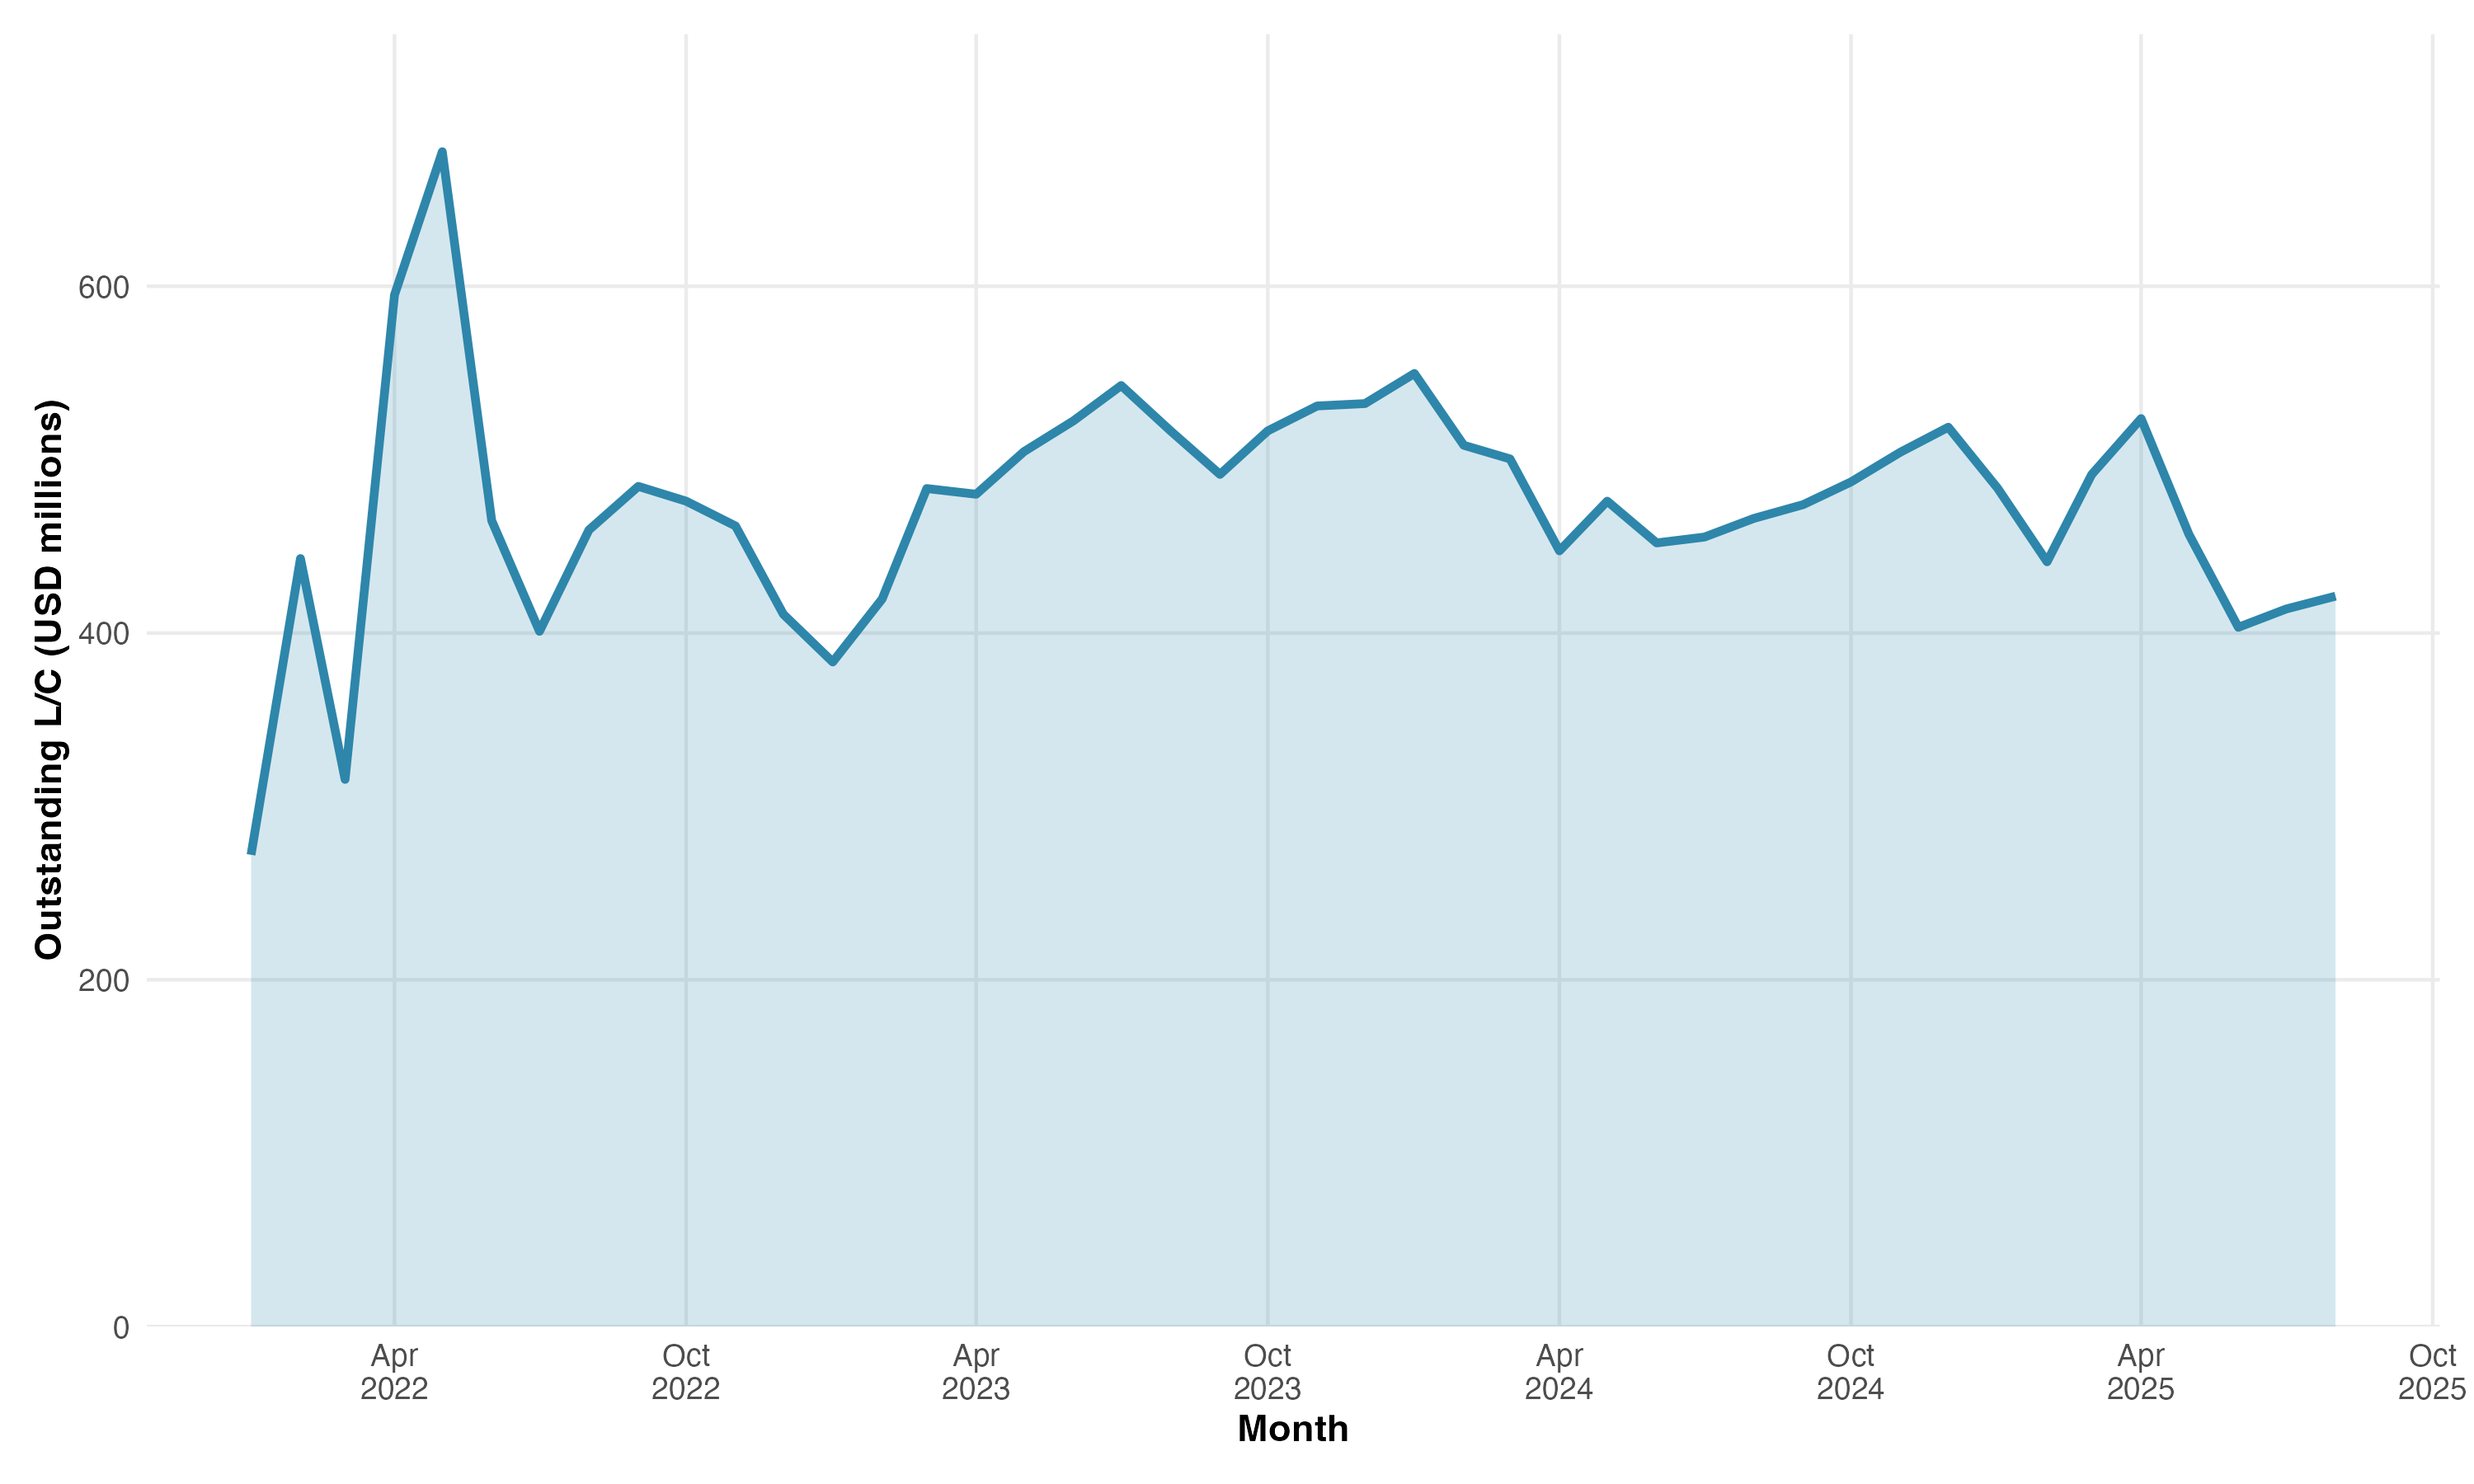
\includegraphics[width=0.7\textwidth]{plots/mexico/mex_01_lc_monthly.png}
\end{center}
\vspace{-0.3cm}
\small
\textbf{Description:} Monthly time series of total outstanding letters of credit issued by Mexican banks in USD millions.

\vspace{0.2cm}
\textbf{Source:} CNBV Reporte A-1219

\vspace{0.2cm}
\textbf{Notes:} Data from account 202401504003 (Import L/C $\leq$ 180 days). Range: USD 272-678 millions.
\end{frame}

\begin{frame}{MEX-2: Letters of Credit as \% of Total Liabilities}
\begin{center}
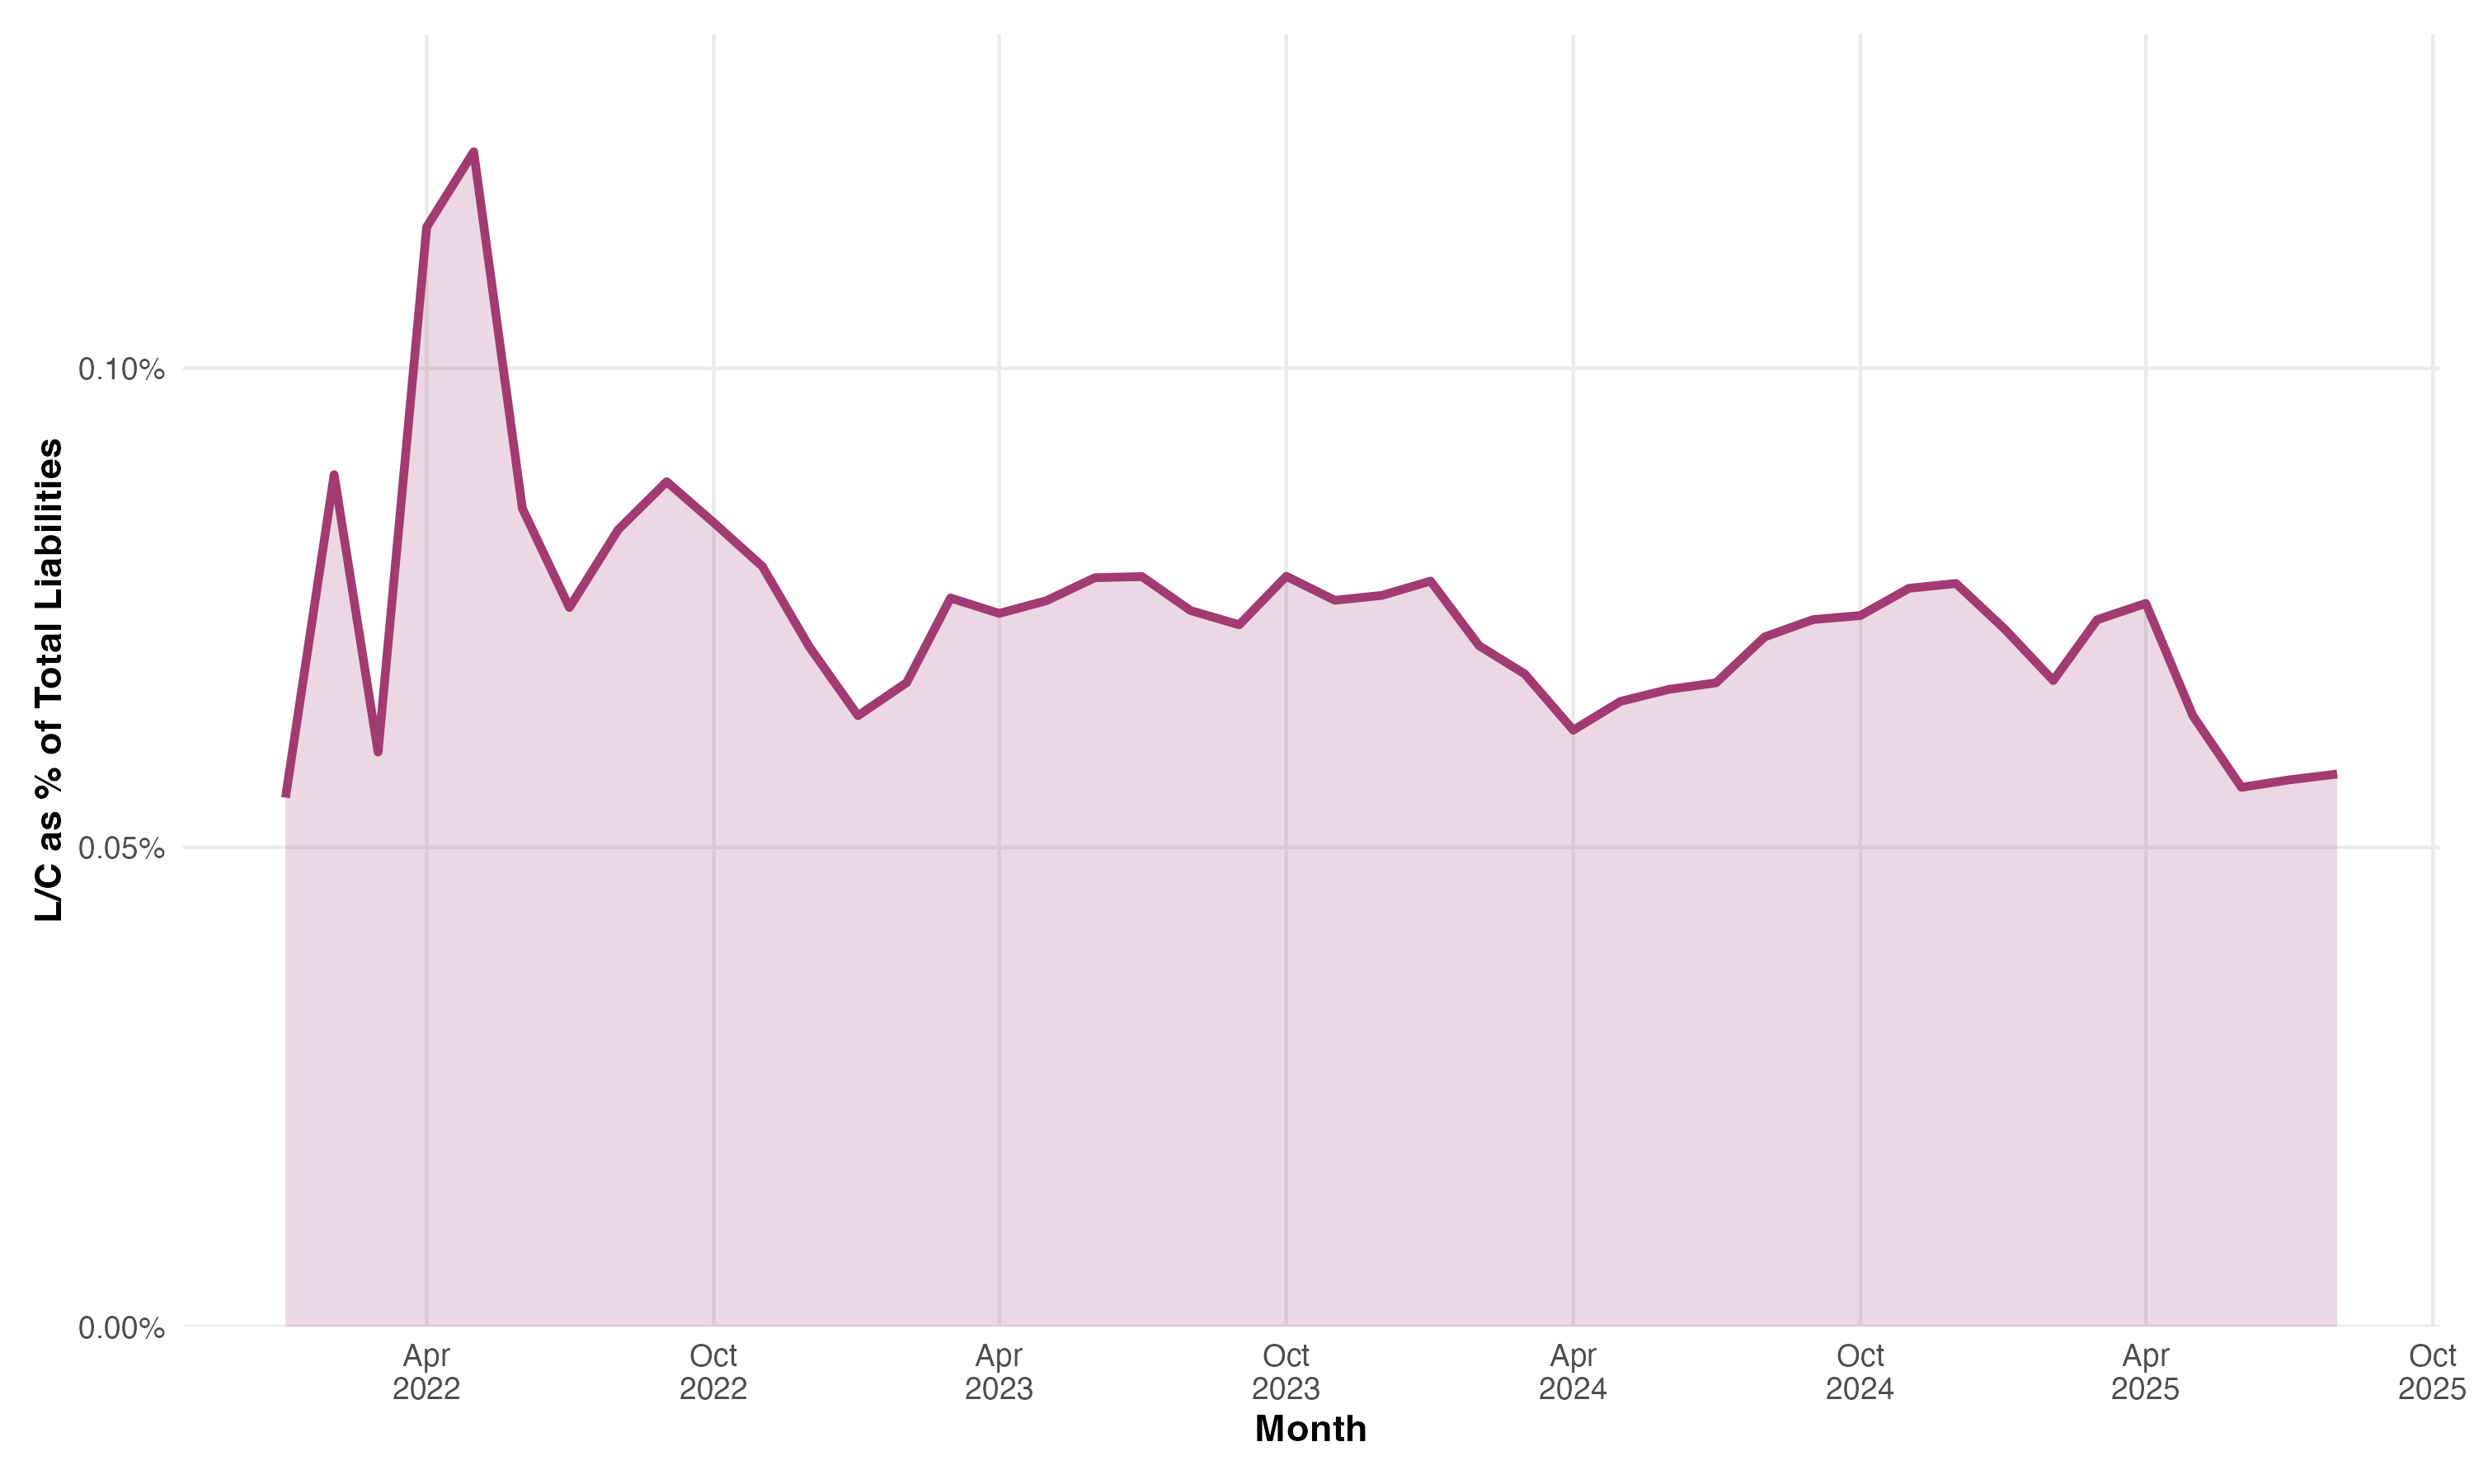
\includegraphics[width=0.7\textwidth]{plots/mexico/mex_02_lc_pct_liabilities.png}
\end{center}
\vspace{-0.3cm}
\small
\textbf{Description:} Letters of credit as percentage of total bank liabilities. Monthly frequency 2022-2025.

\vspace{0.2cm}
\textbf{Source:} CNBV Reporte A-1219

\vspace{0.2cm}
\textbf{Notes:} Range: 0.055\%-0.123\%.
\end{frame}

\begin{frame}{MEX-3: Letters of Credit by Type of Bank}
\begin{center}
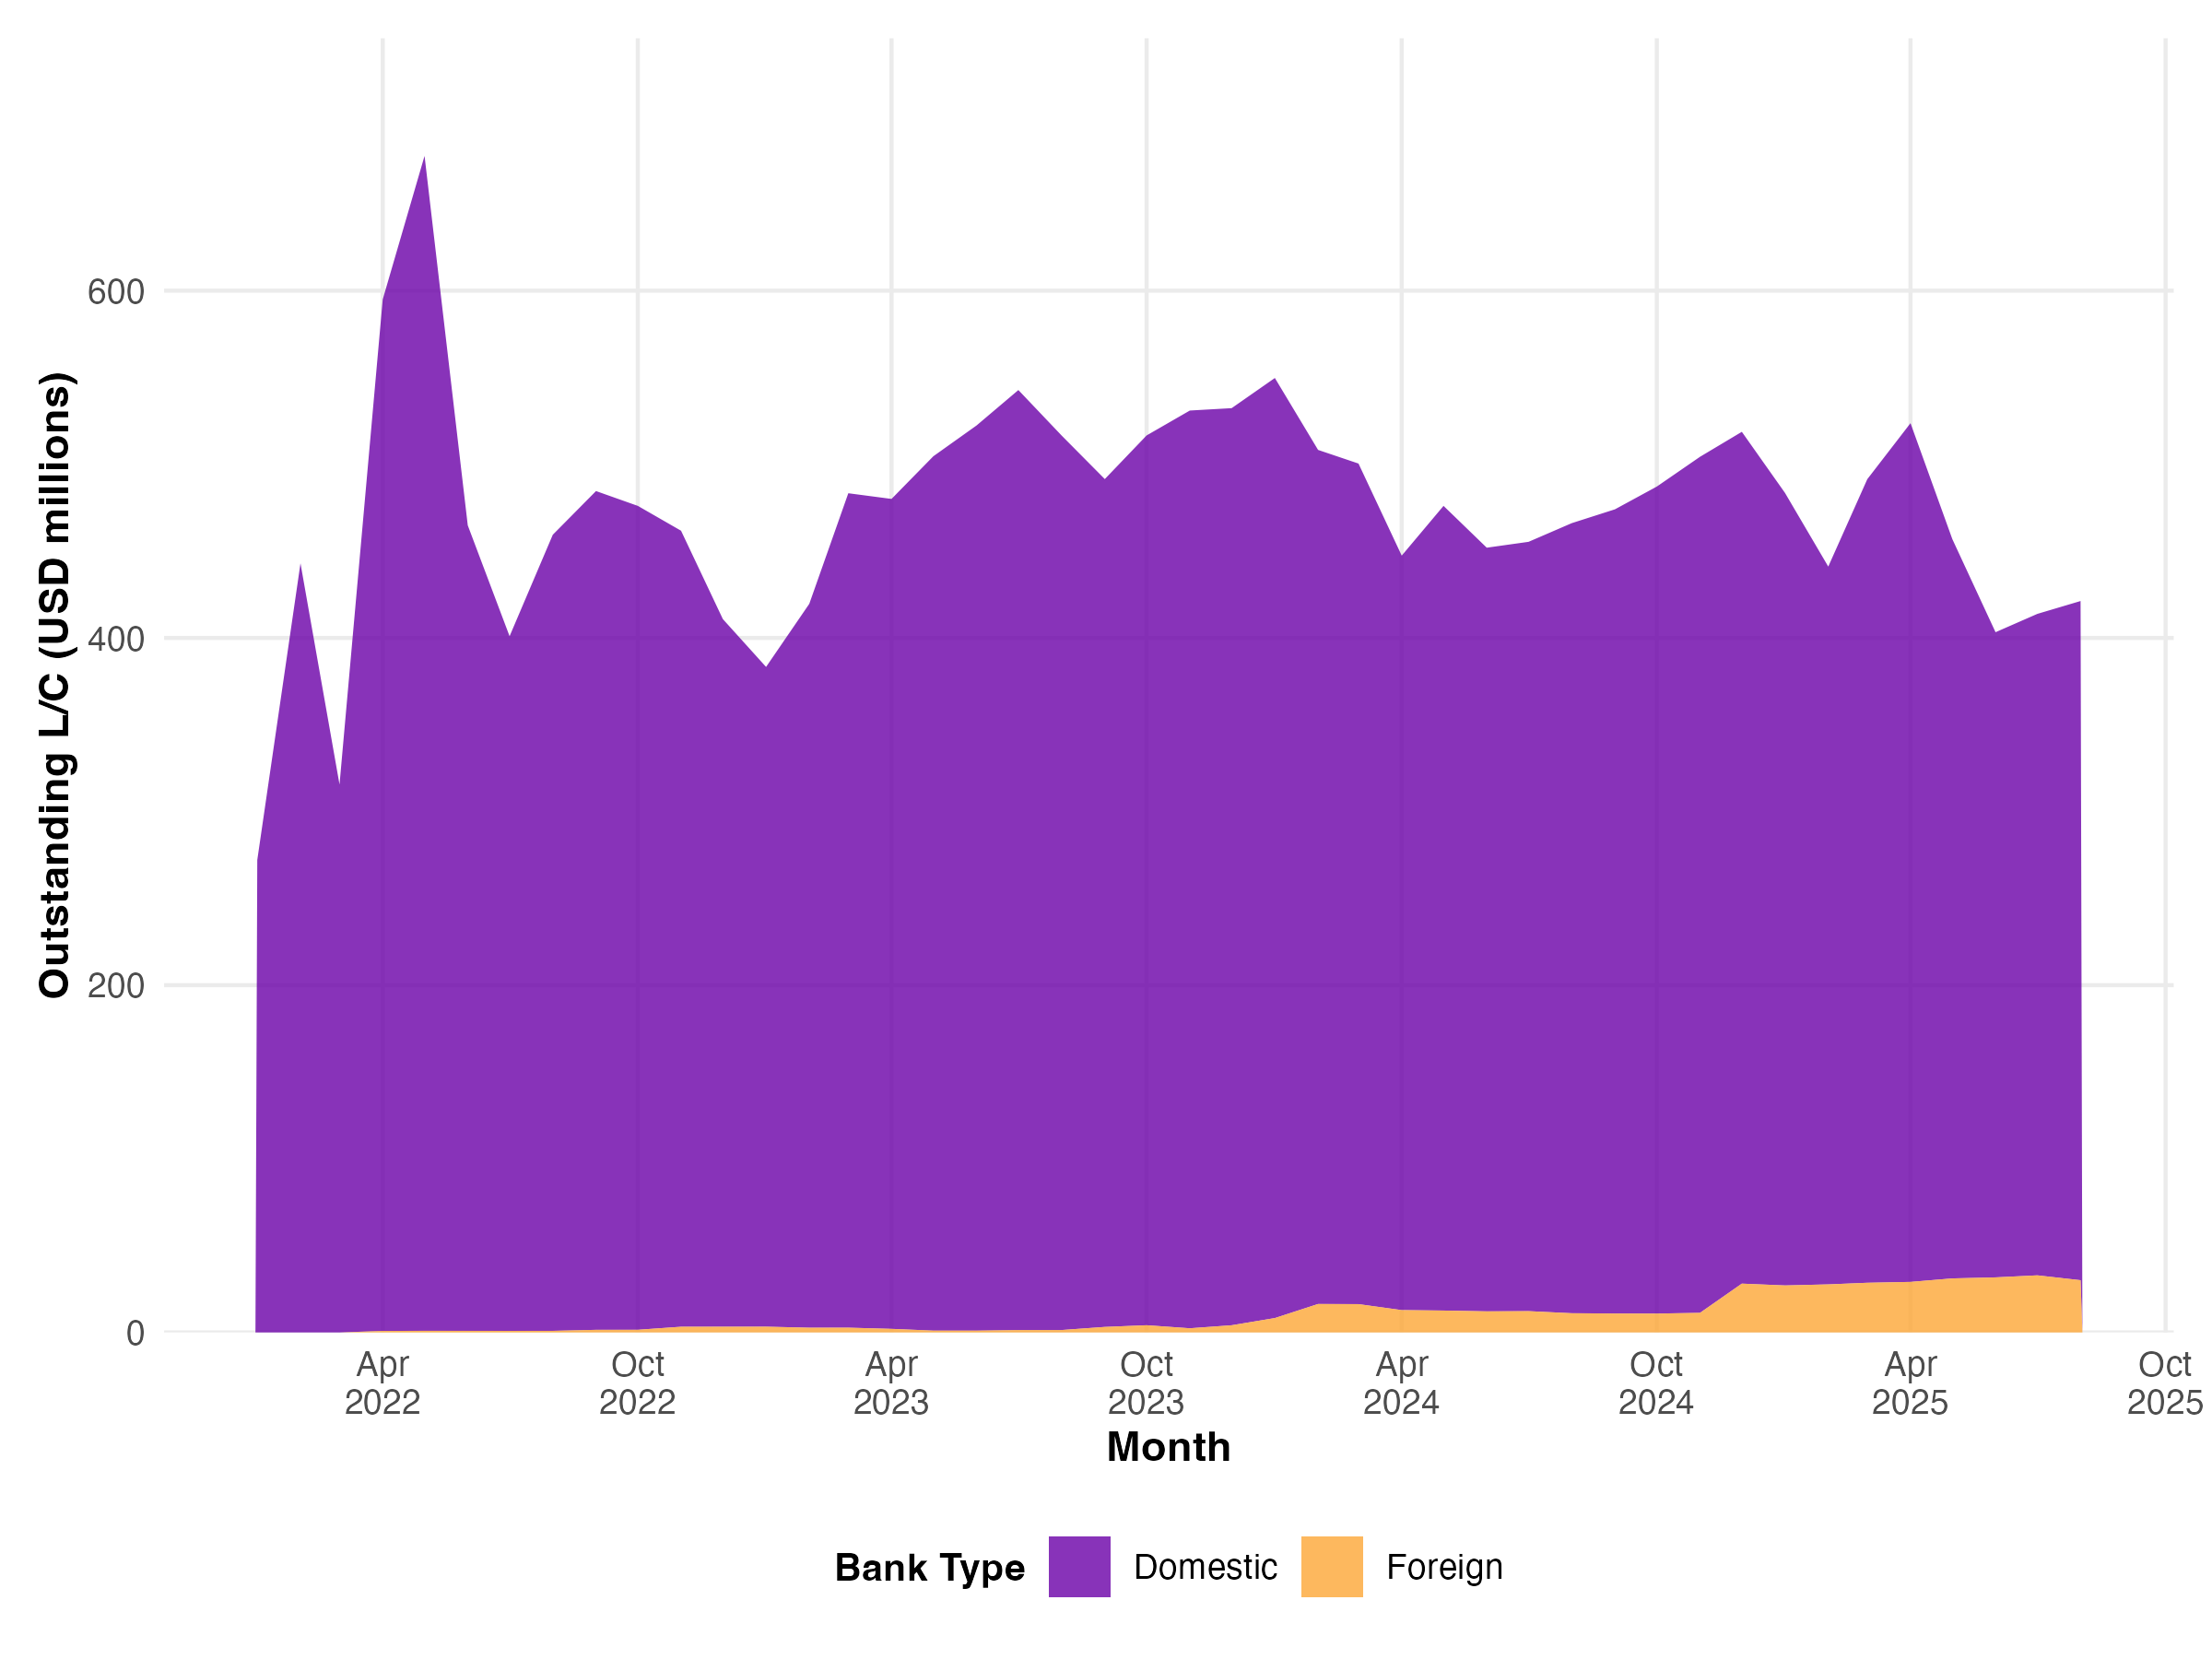
\includegraphics[width=0.7\textwidth]{plots/mexico/mex_03_lc_by_bank_type.png}
\end{center}
\vspace{-0.3cm}
\small
\textbf{Description:} Distribution of outstanding L/C across Foreign and Domestic banks. Stacked area chart 2022-2025.

\vspace{0.2cm}
\textbf{Source:} CNBV Reporte A-1219

\vspace{0.2cm}
\textbf{Notes:} Domestic banks: 98\% of cumulative L/C volume (USD 20.4B total). Foreign banks: 2\% (USD 445M).
\end{frame}

\begin{frame}{MEX-4: L/C as \% of Annual Exports}
\begin{center}
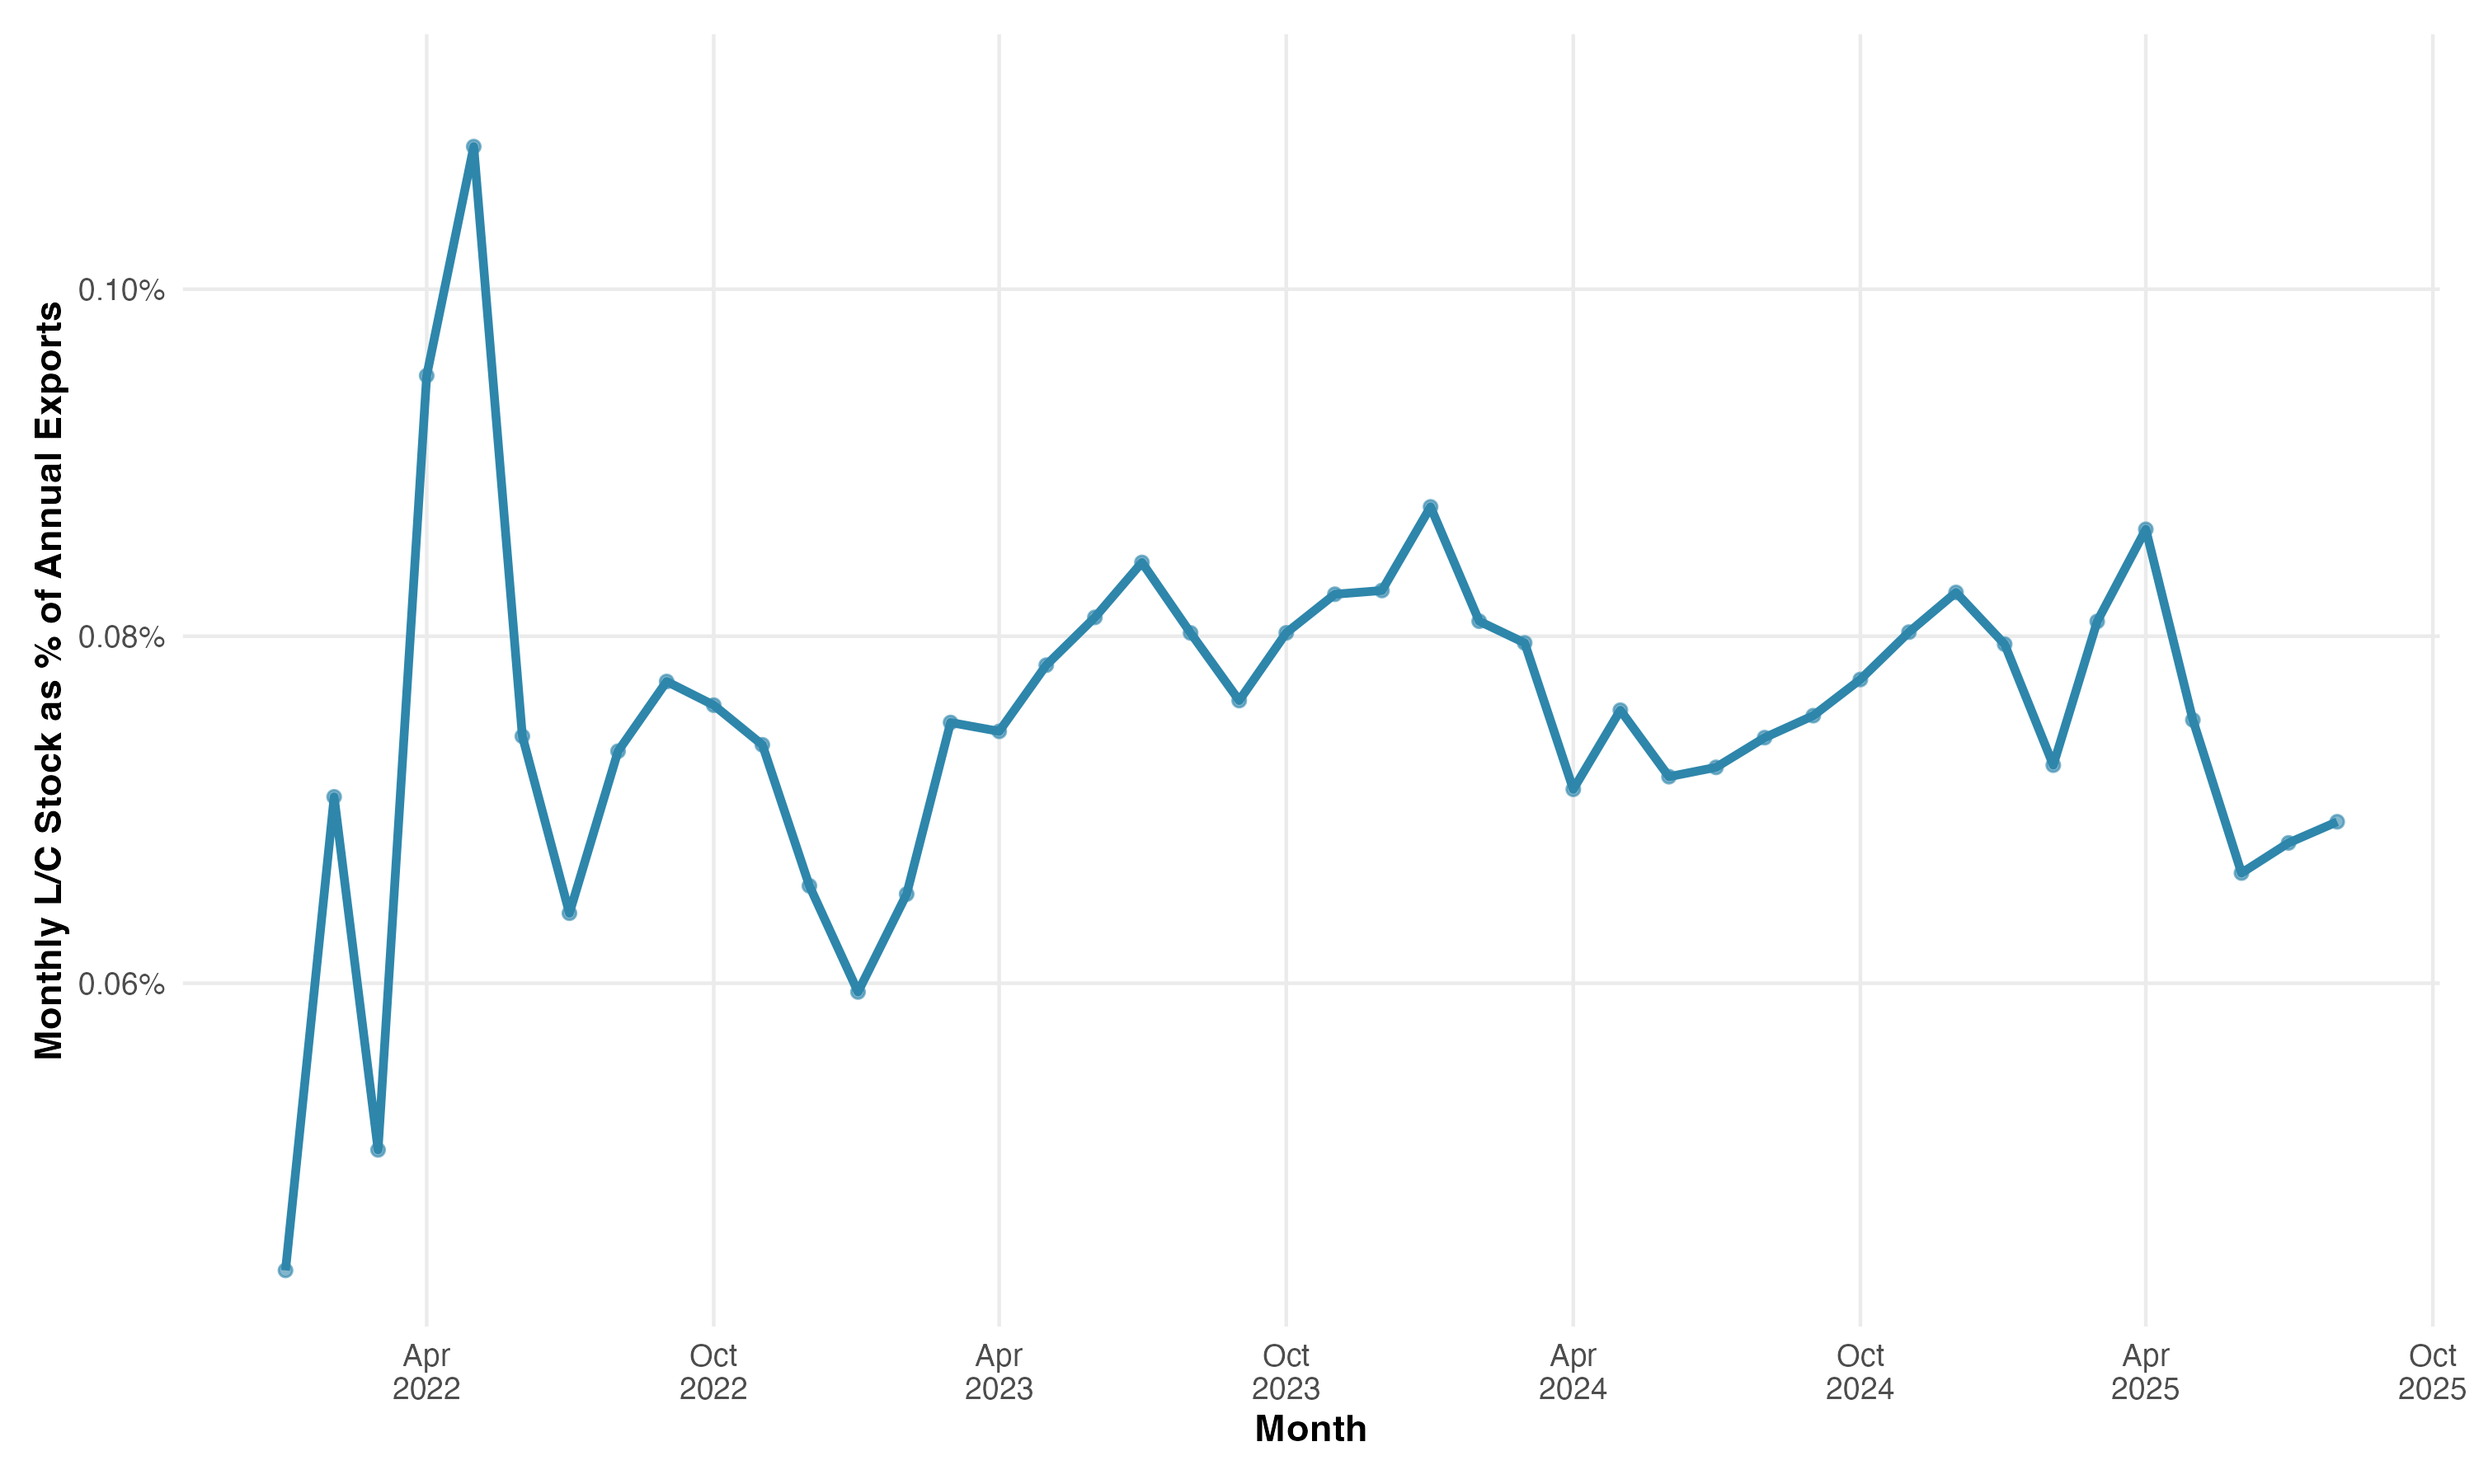
\includegraphics[width=0.7\textwidth]{plots/mexico/mex_04_lc_pct_exports.png}
\end{center}
\vspace{-0.3cm}
\small
\textbf{Description:} Monthly L/C stock as percentage of annual exports. Methodology: monthly stock / annual exports × 100.

\vspace{0.2cm}
\textbf{Source:} CNBV Reporte A-1219 + GMD

\vspace{0.2cm}
\textbf{Notes:} Range: 0.043\%-0.108\%.
\end{frame}

\begin{frame}{MEX-5: L/C as \% of Annual Total Trade}
\begin{center}
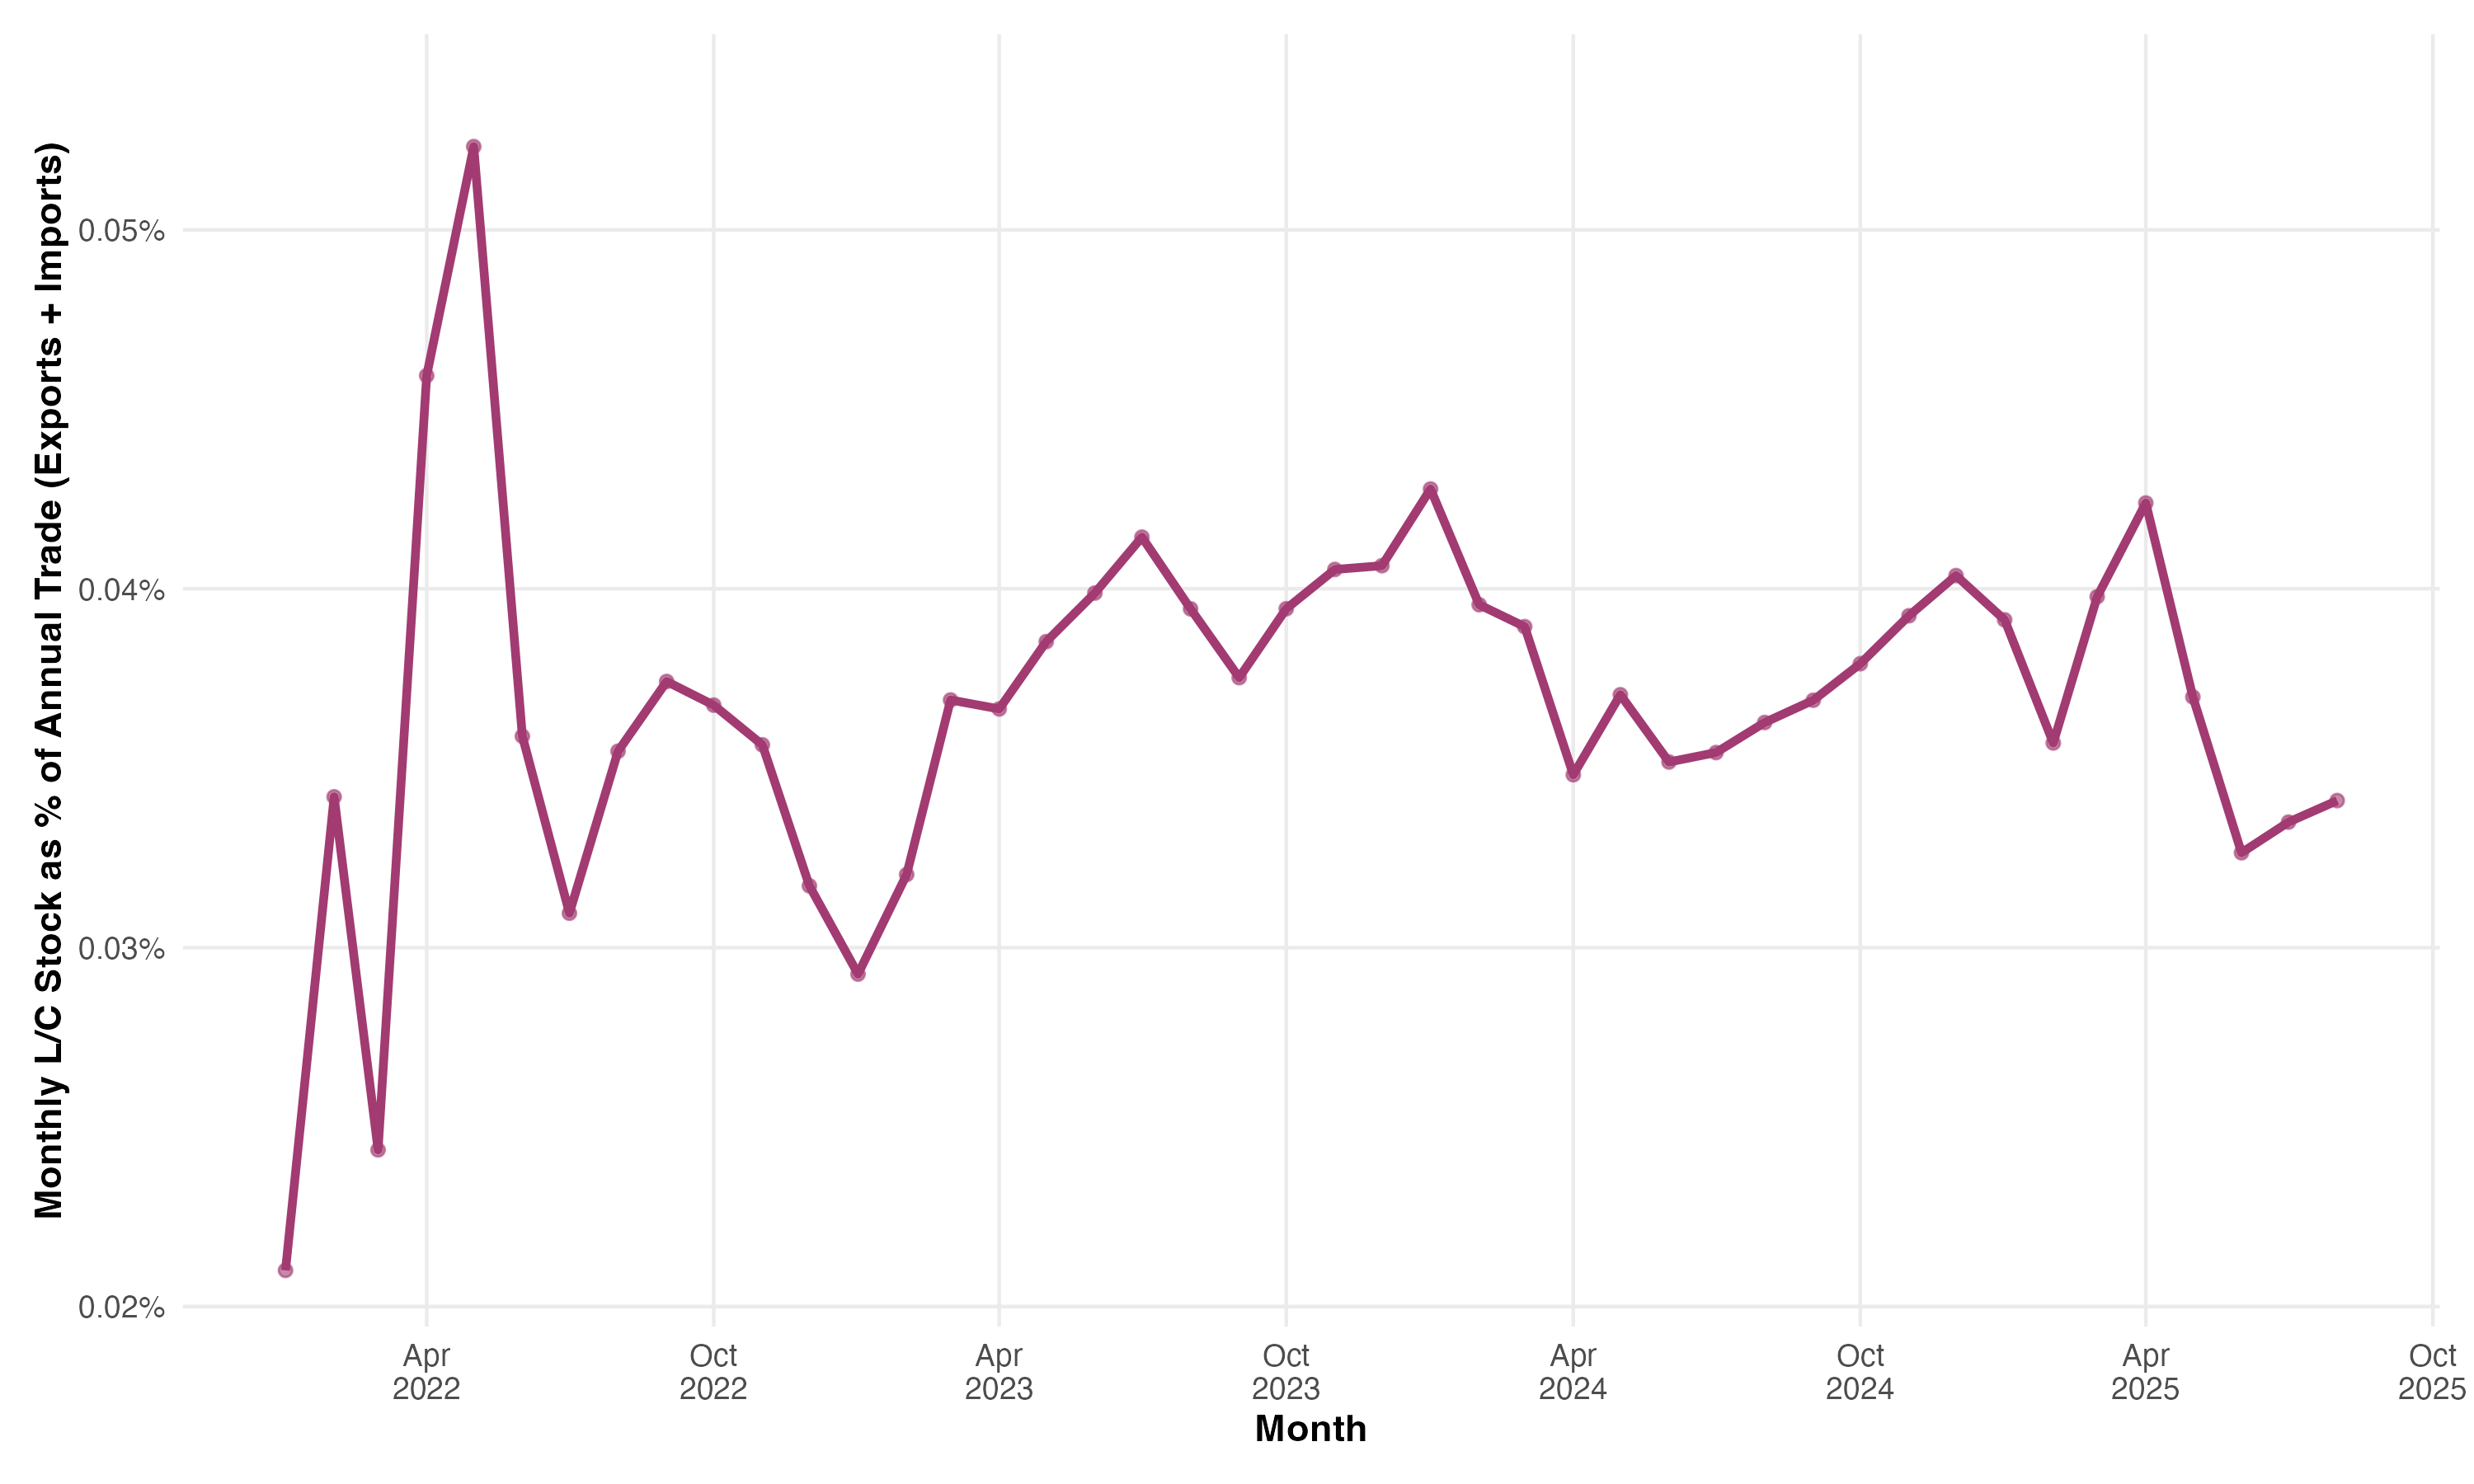
\includegraphics[width=0.7\textwidth]{plots/mexico/mex_05_lc_pct_trade.png}
\end{center}
\vspace{-0.3cm}
\small
\textbf{Description:} Monthly L/C stock as percentage of annual total trade (exports + imports). Methodology: monthly stock / annual (X+M) × 100.

\vspace{0.2cm}
\textbf{Source:} CNBV Reporte A-1219 + GMD

\vspace{0.2cm}
\textbf{Notes:} Range: 0.021\%-0.052\%.
\end{frame}

\begin{frame}{MEX-6: L/C by Top 5 Banks (Monthly)}
\begin{center}
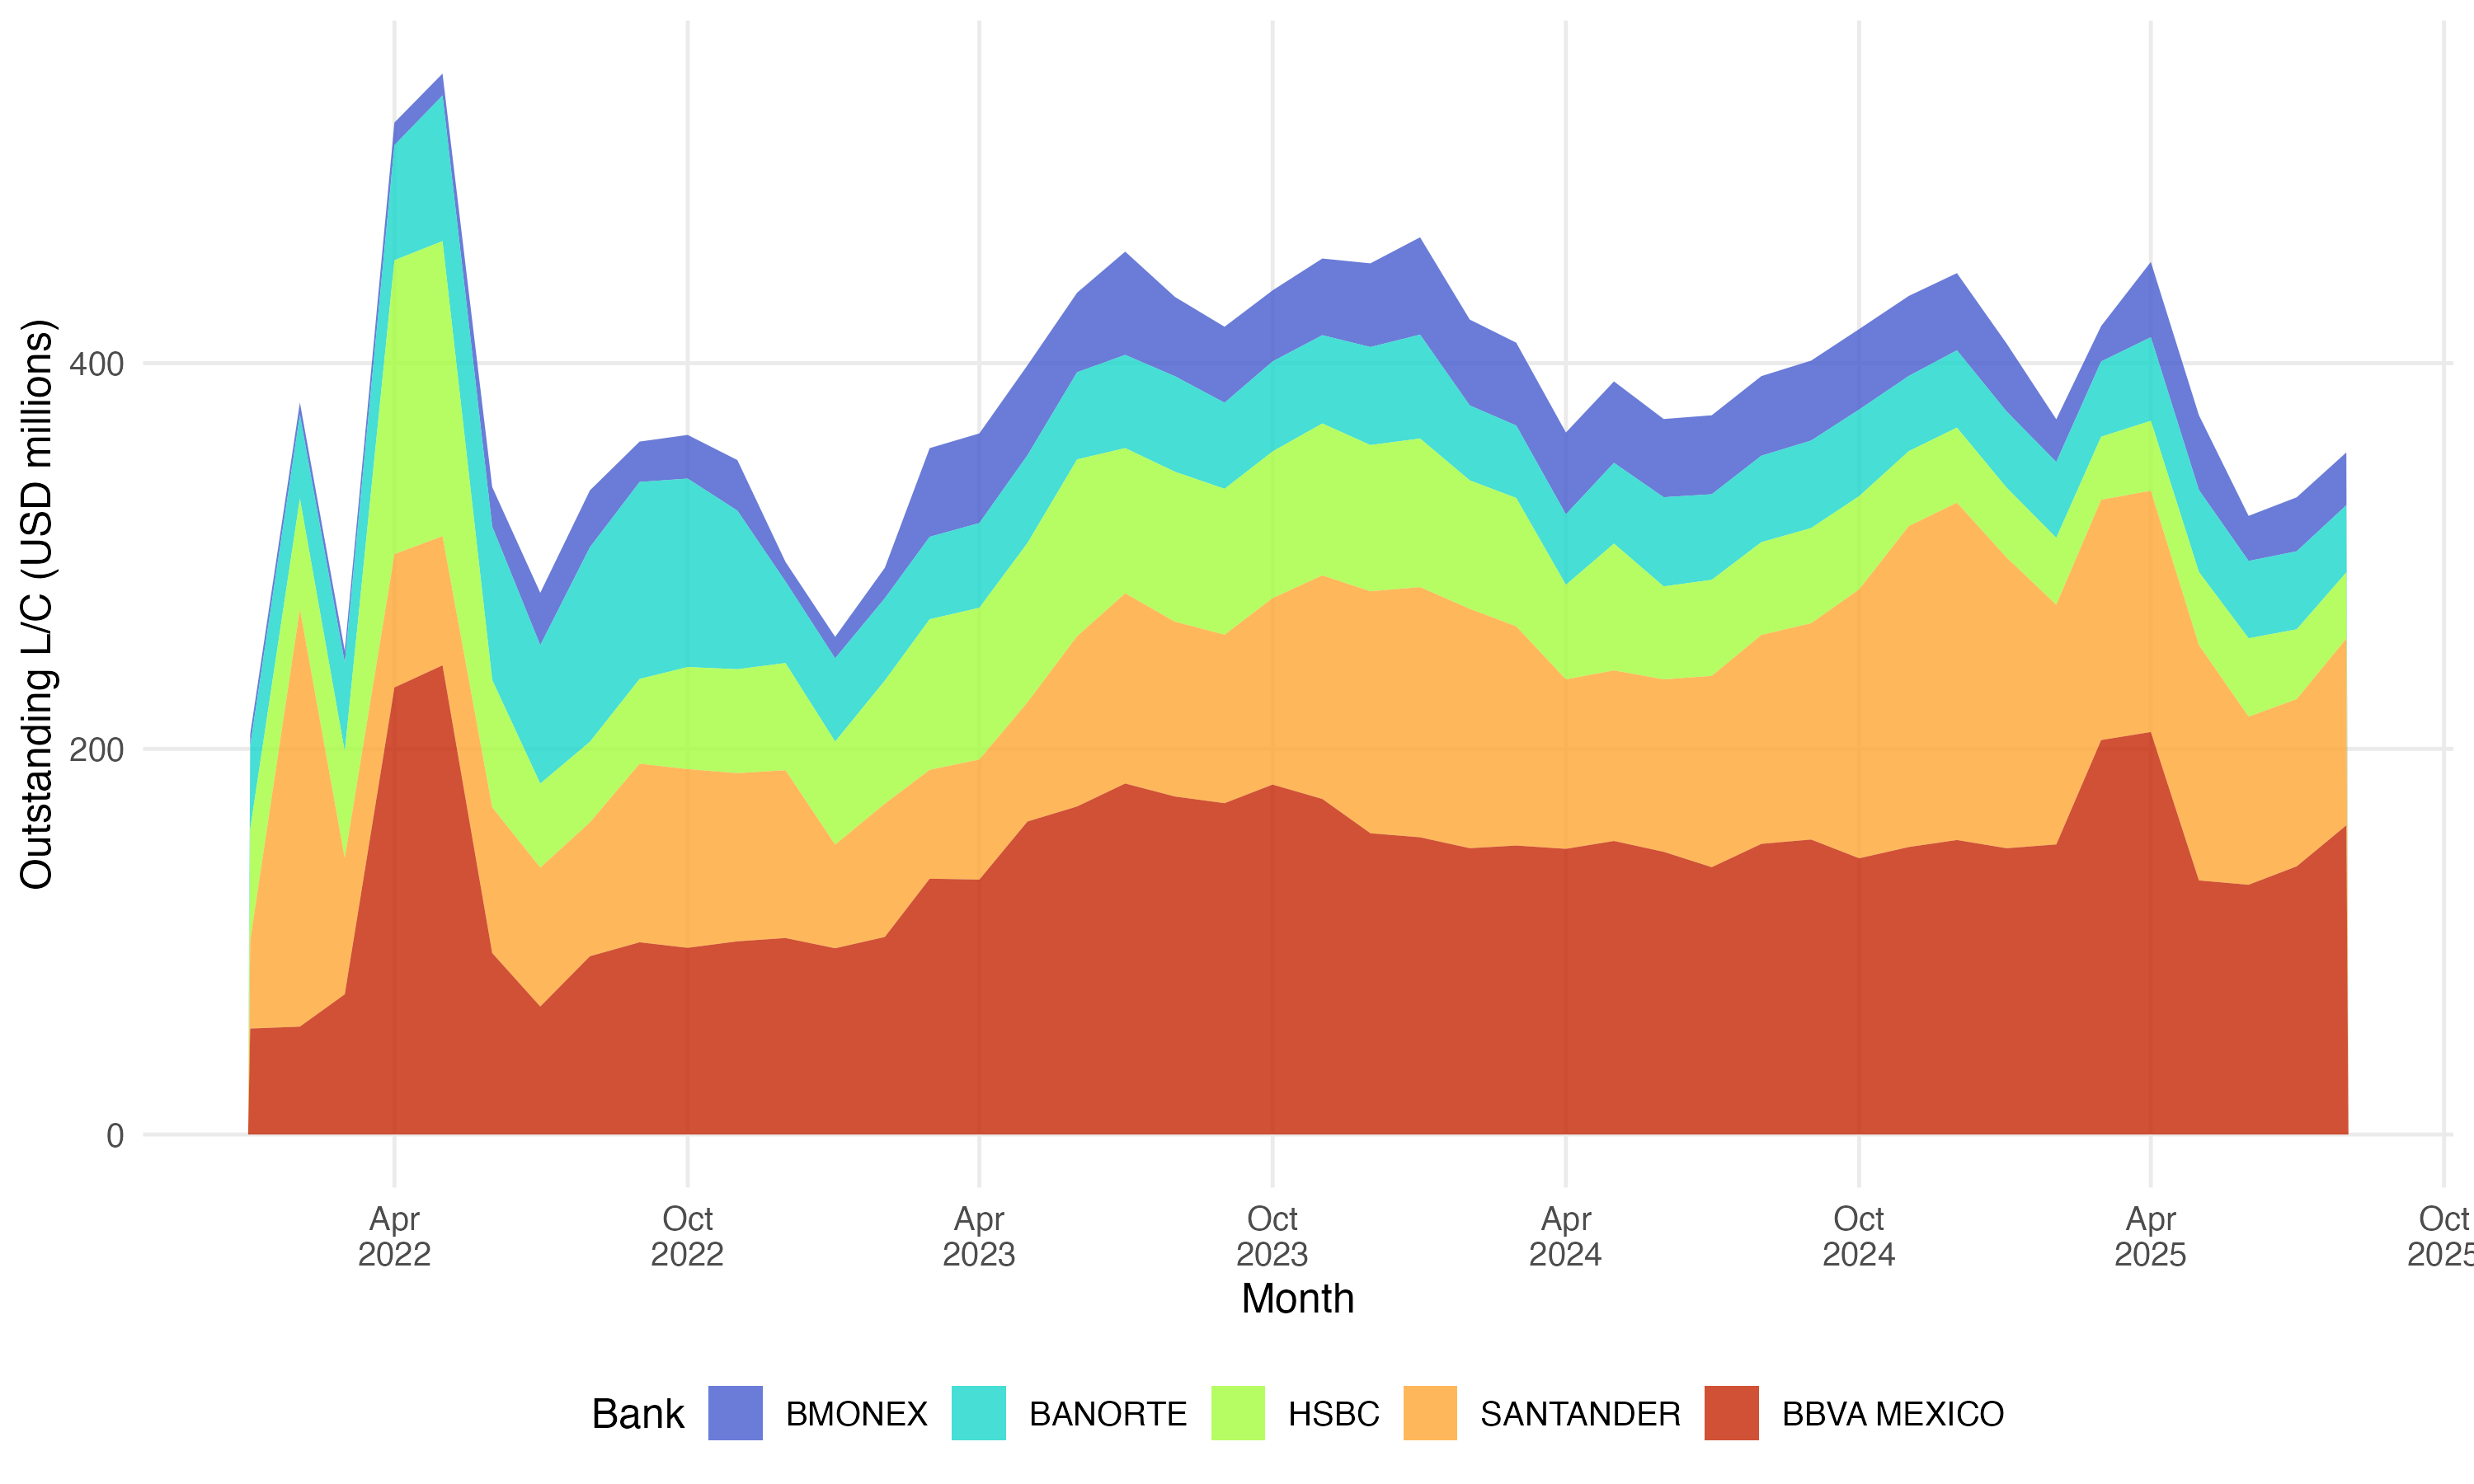
\includegraphics[width=0.7\textwidth]{plots/mexico/mex_06_lc_top5_banks.png}
\end{center}
\vspace{-0.3cm}
\small
\textbf{Description:} Monthly stacked area showing L/C concentration among top 5 issuing banks. 2022-2025.

\vspace{0.2cm}
\textbf{Source:} CNBV Reporte A-1219

\vspace{0.2cm}
\textbf{Notes:} Top 5 banks account for majority of L/C market.
\end{frame}

% ==============================================================================
% SECTION 3: PERU GRAPHS
% ==============================================================================

\section{Peru}

% Country separator slide
\begin{frame}
\begin{center}
\vspace{2cm}
{\Huge \textbf{PERU}}

\vspace{0.5cm}
{\Large Trade Finance Analysis}

\vspace{1cm}
\large
7 Graphs | 2010-2024 | SBS Balance de Comprobación

\vspace{0.3cm}
\normalsize
Foreign-Trade Credit (Comercio Exterior)
\end{center}
\end{frame}

\begin{frame}{PER-1: Foreign-Trade Credit as \% of Total Credit}
\begin{center}
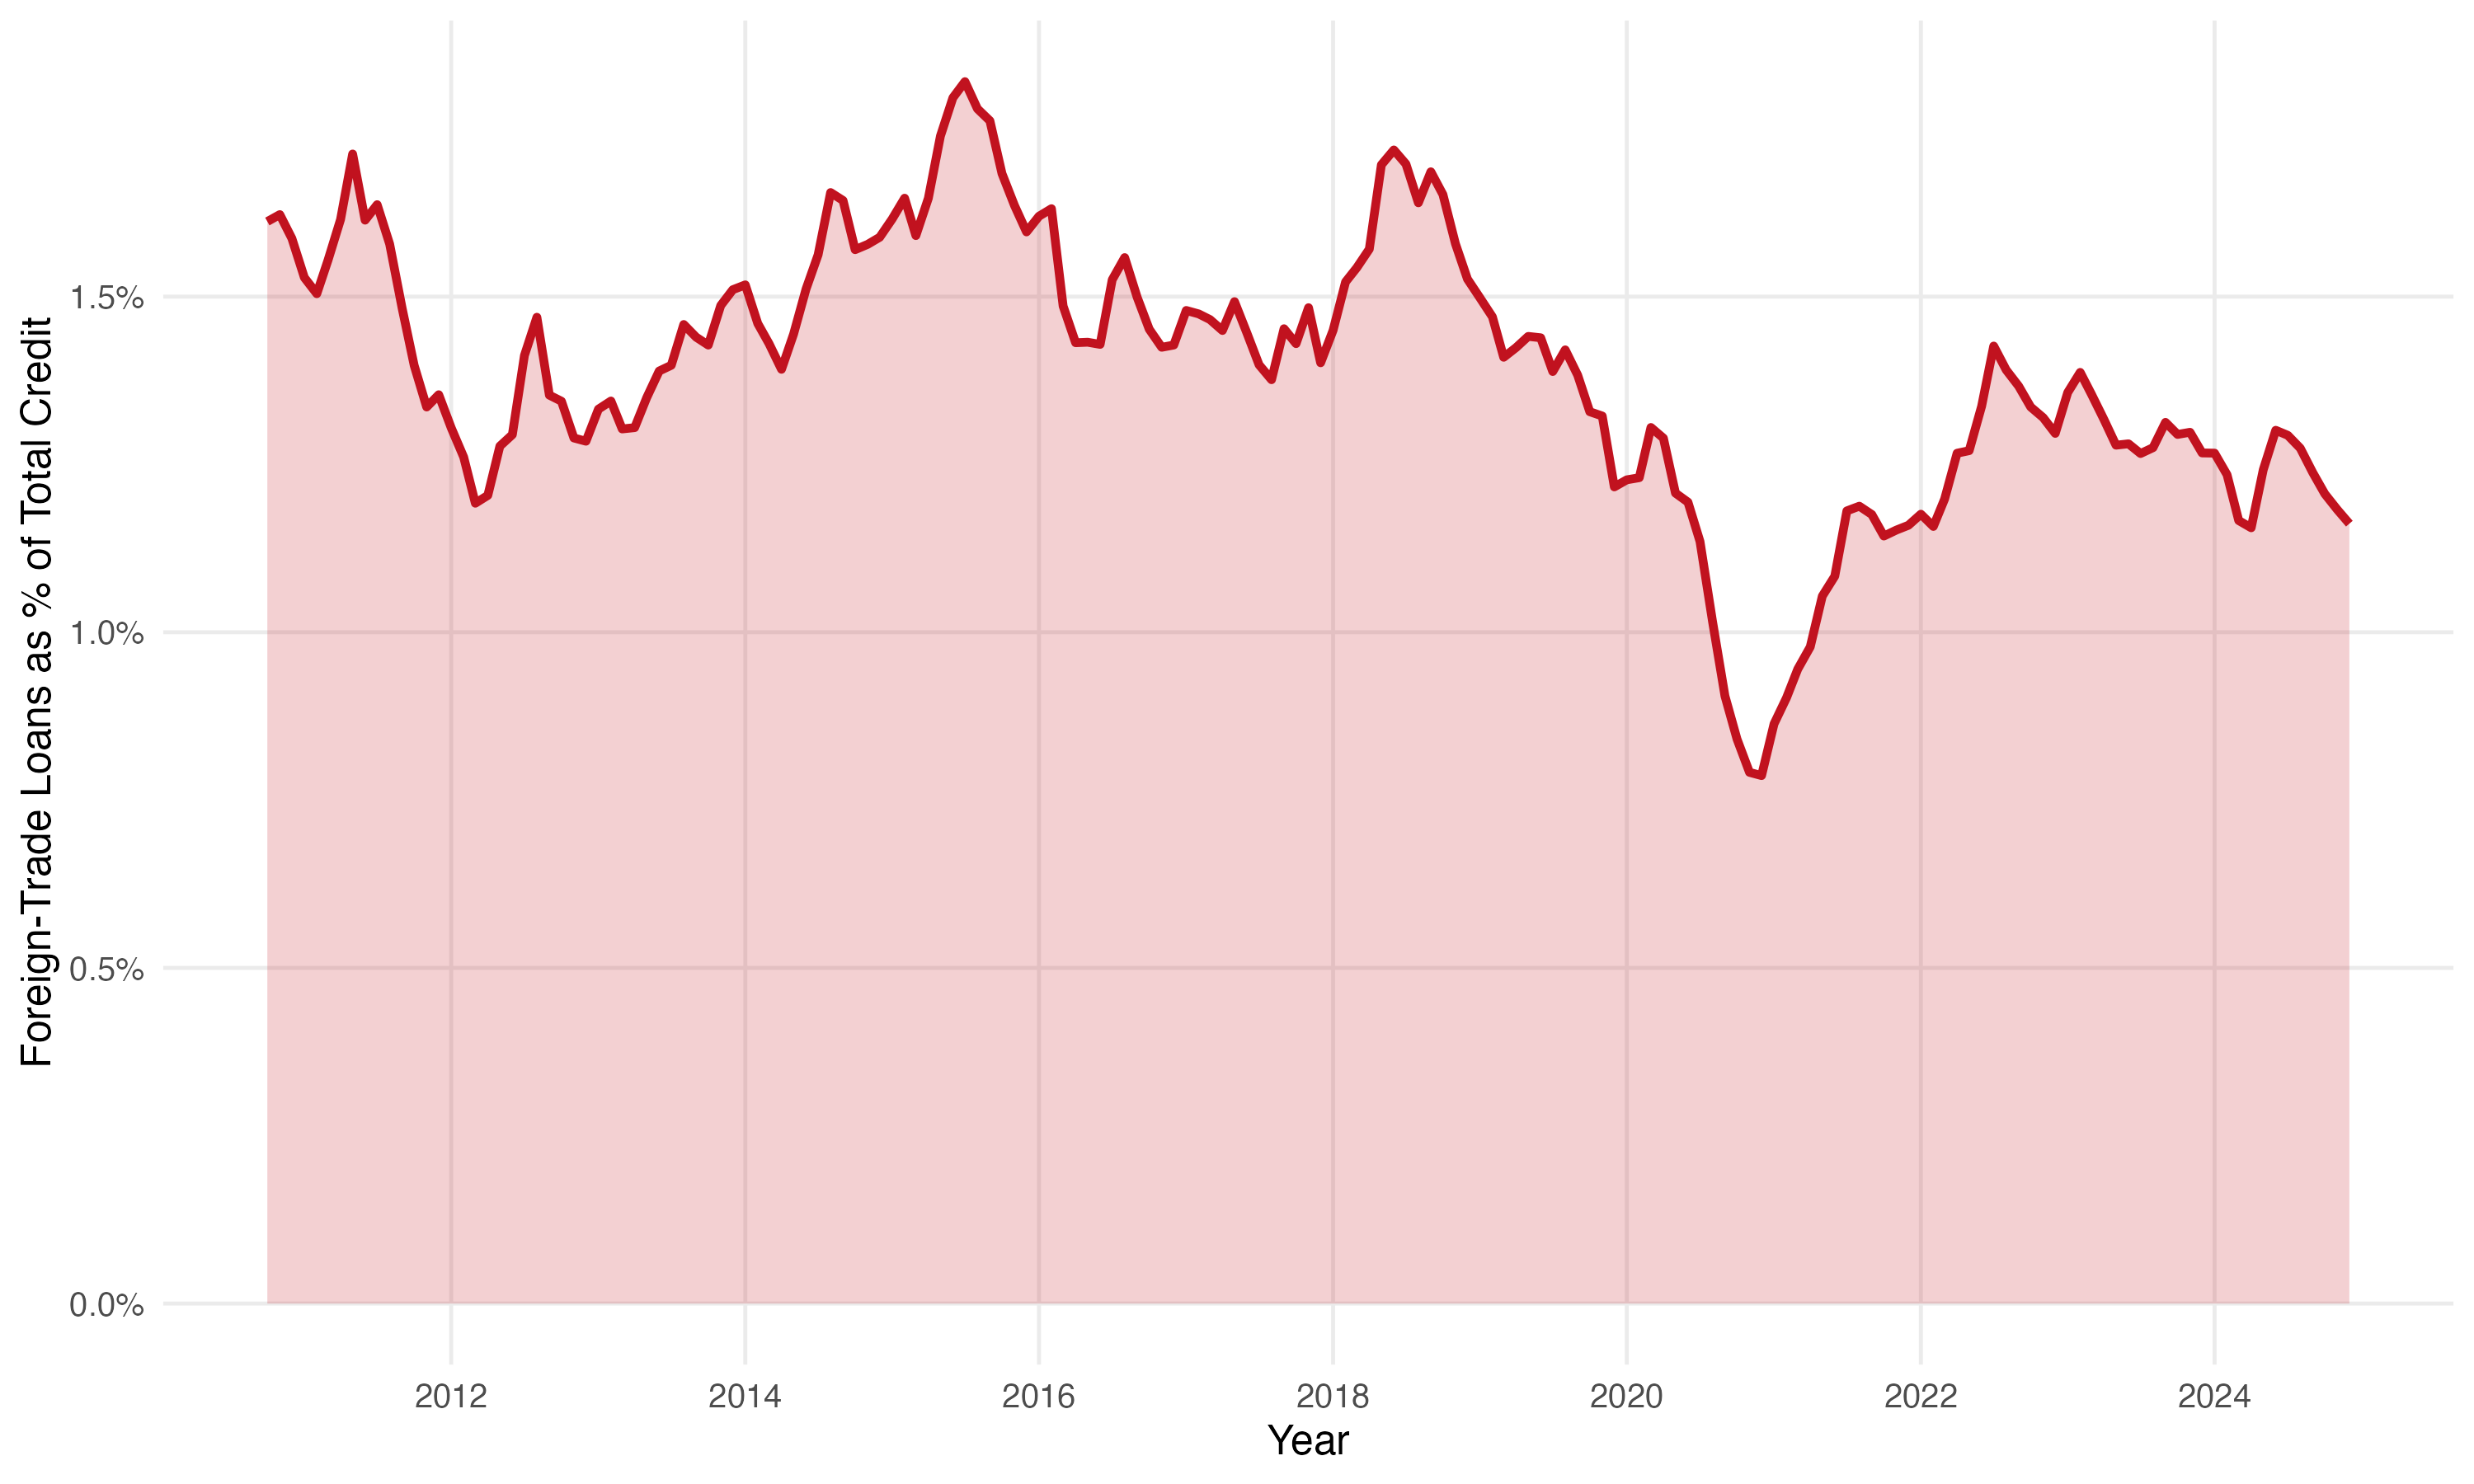
\includegraphics[width=0.7\textwidth]{plots/peru/per_01_tf_pct_total.png}
\end{center}
\vspace{-0.3cm}
\small
\textbf{Description:} Foreign-trade credit as share of total credit portfolio. Monthly 2010-2024.

\vspace{0.2cm}
\textbf{Source:} SBS Credit Registry

\vspace{0.2cm}
\textbf{Notes:} Range: 3-7\% of total credit.
\end{frame}

\begin{frame}{PER-2: Foreign-Trade Credit by Borrower Size}
\begin{center}
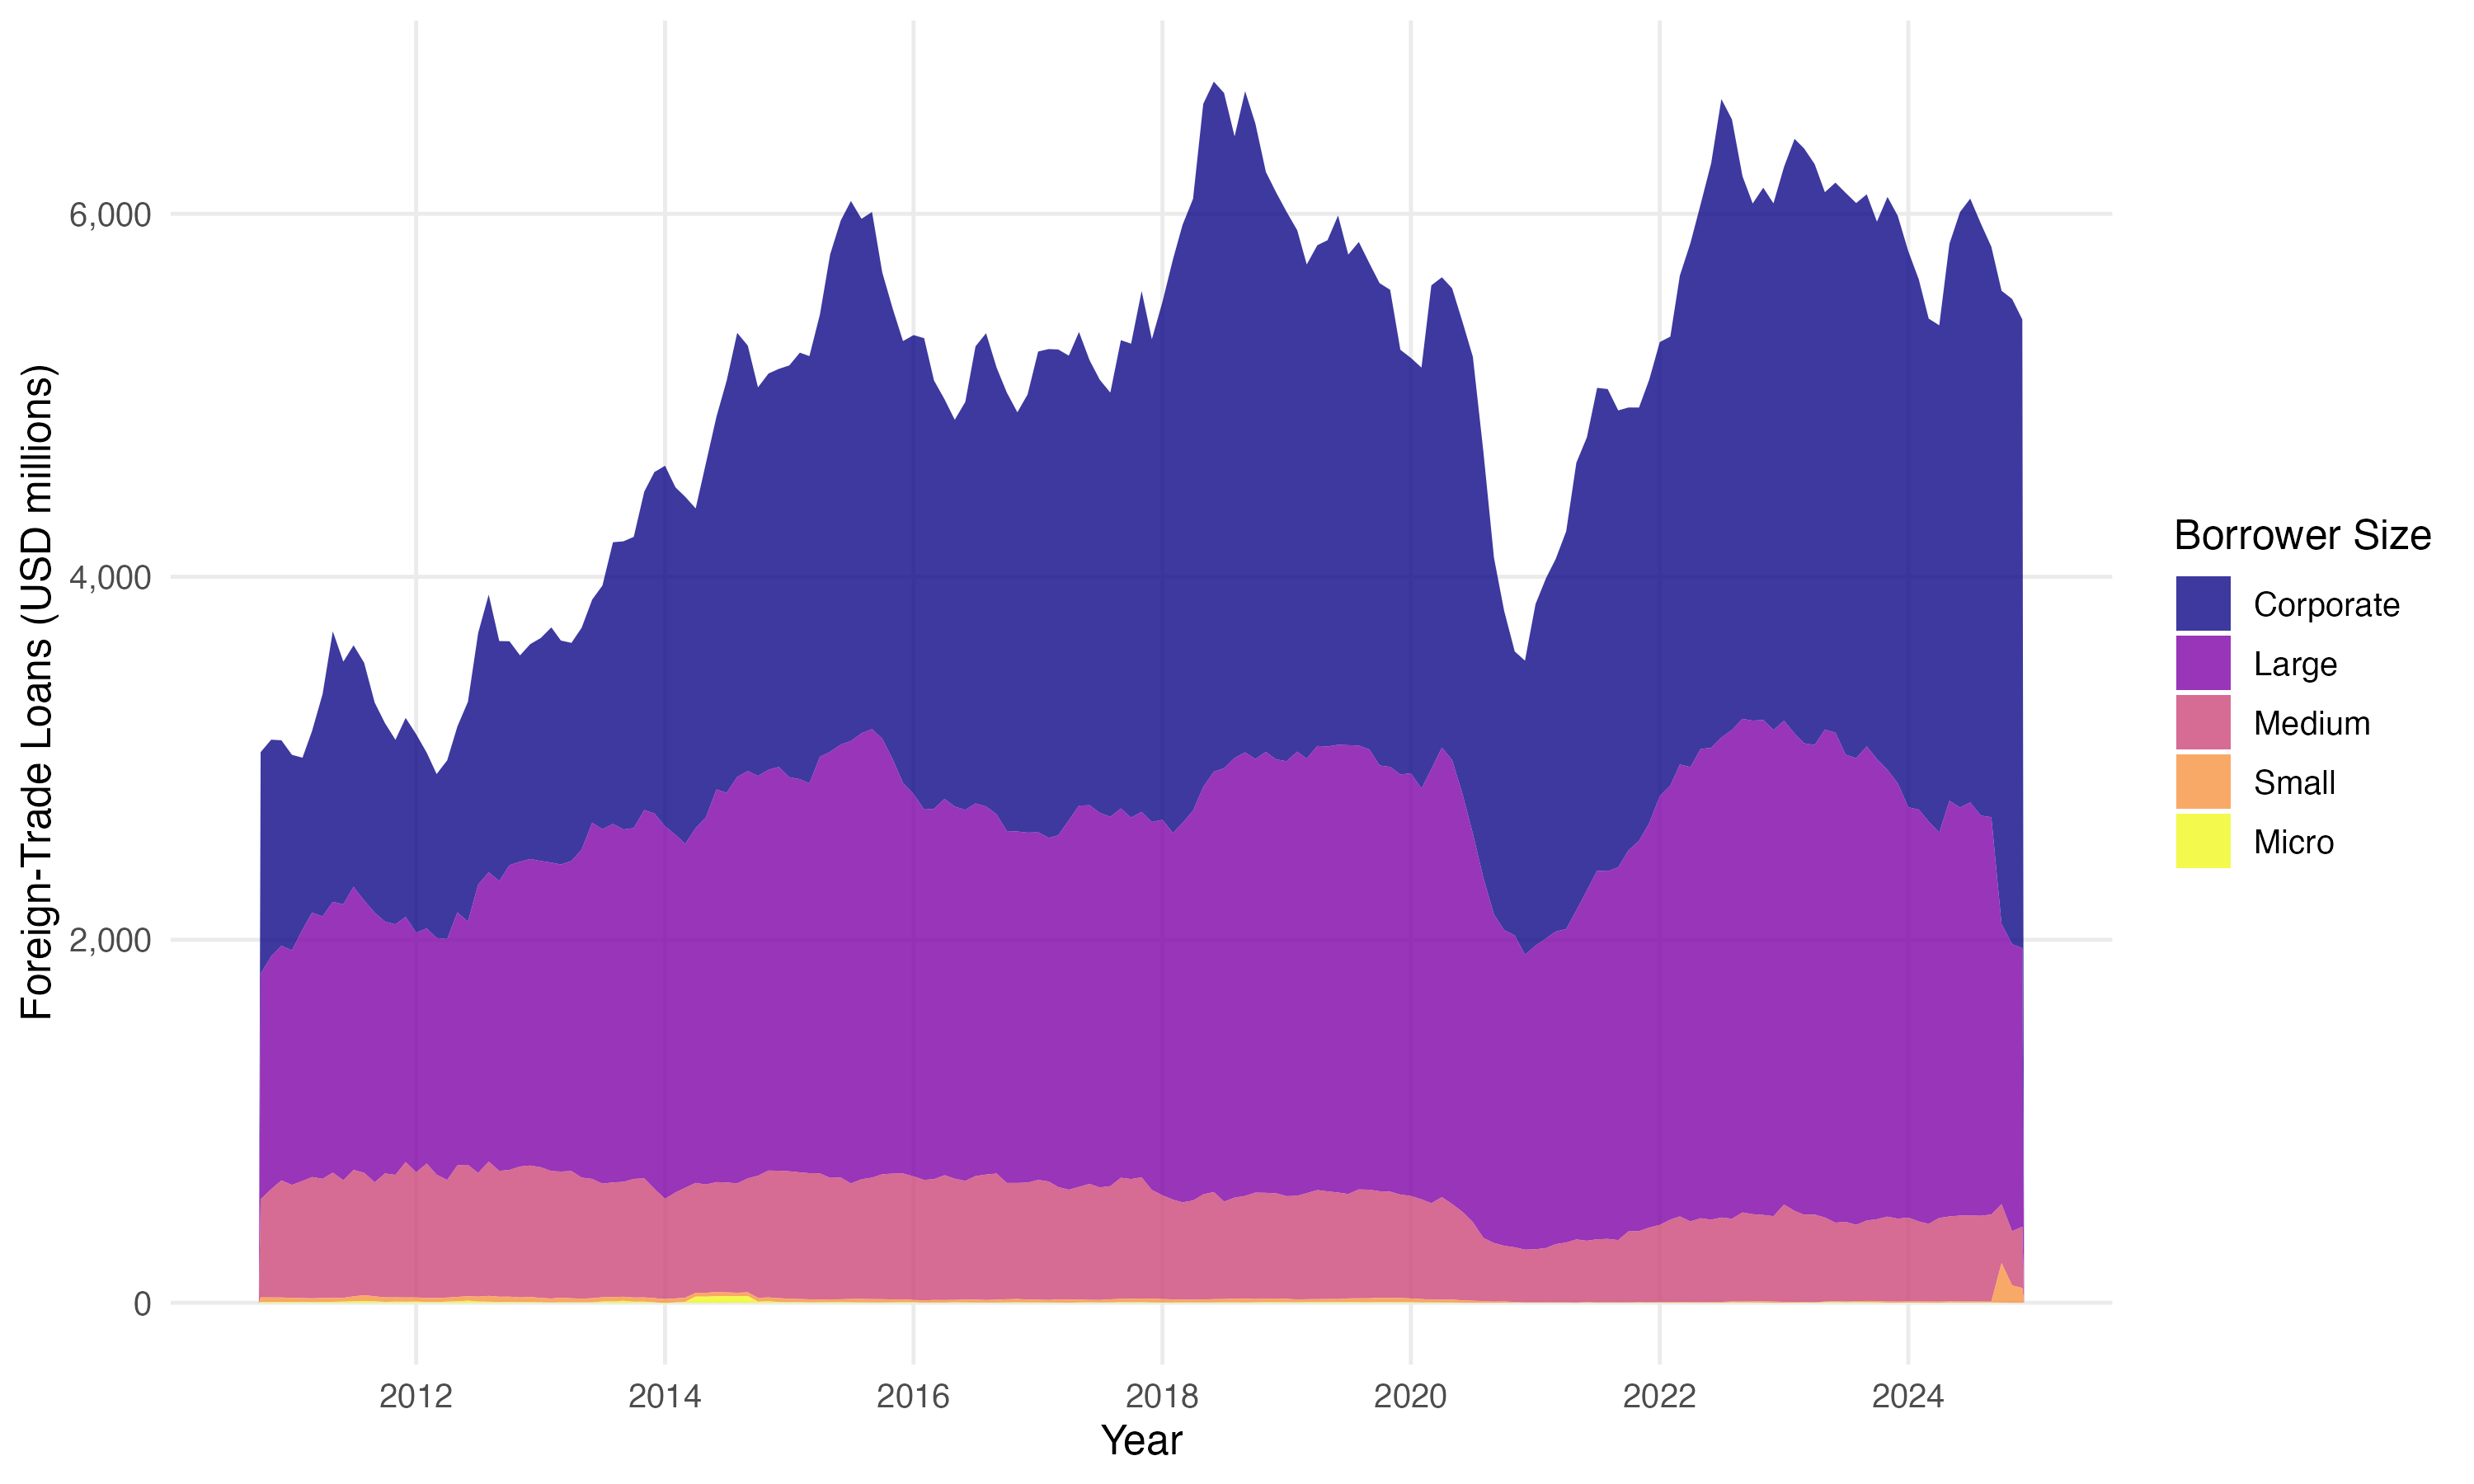
\includegraphics[width=0.7\textwidth]{plots/peru/per_02_tf_by_size.png}
\end{center}
\vspace{-0.3cm}
\small
\textbf{Description:} Annual grouped bars showing TF distribution across borrower size categories. 2010-2024.

\vspace{0.2cm}
\textbf{Source:} SBS Balance de Comprobación

\vspace{0.2cm}
\textbf{Notes:} Five size categories: Micro, Small, Medium, Large, Corporate.
\end{frame}

\begin{frame}{PER-3: Foreign-Trade Credit by Type of Bank (Monthly)}
\begin{center}
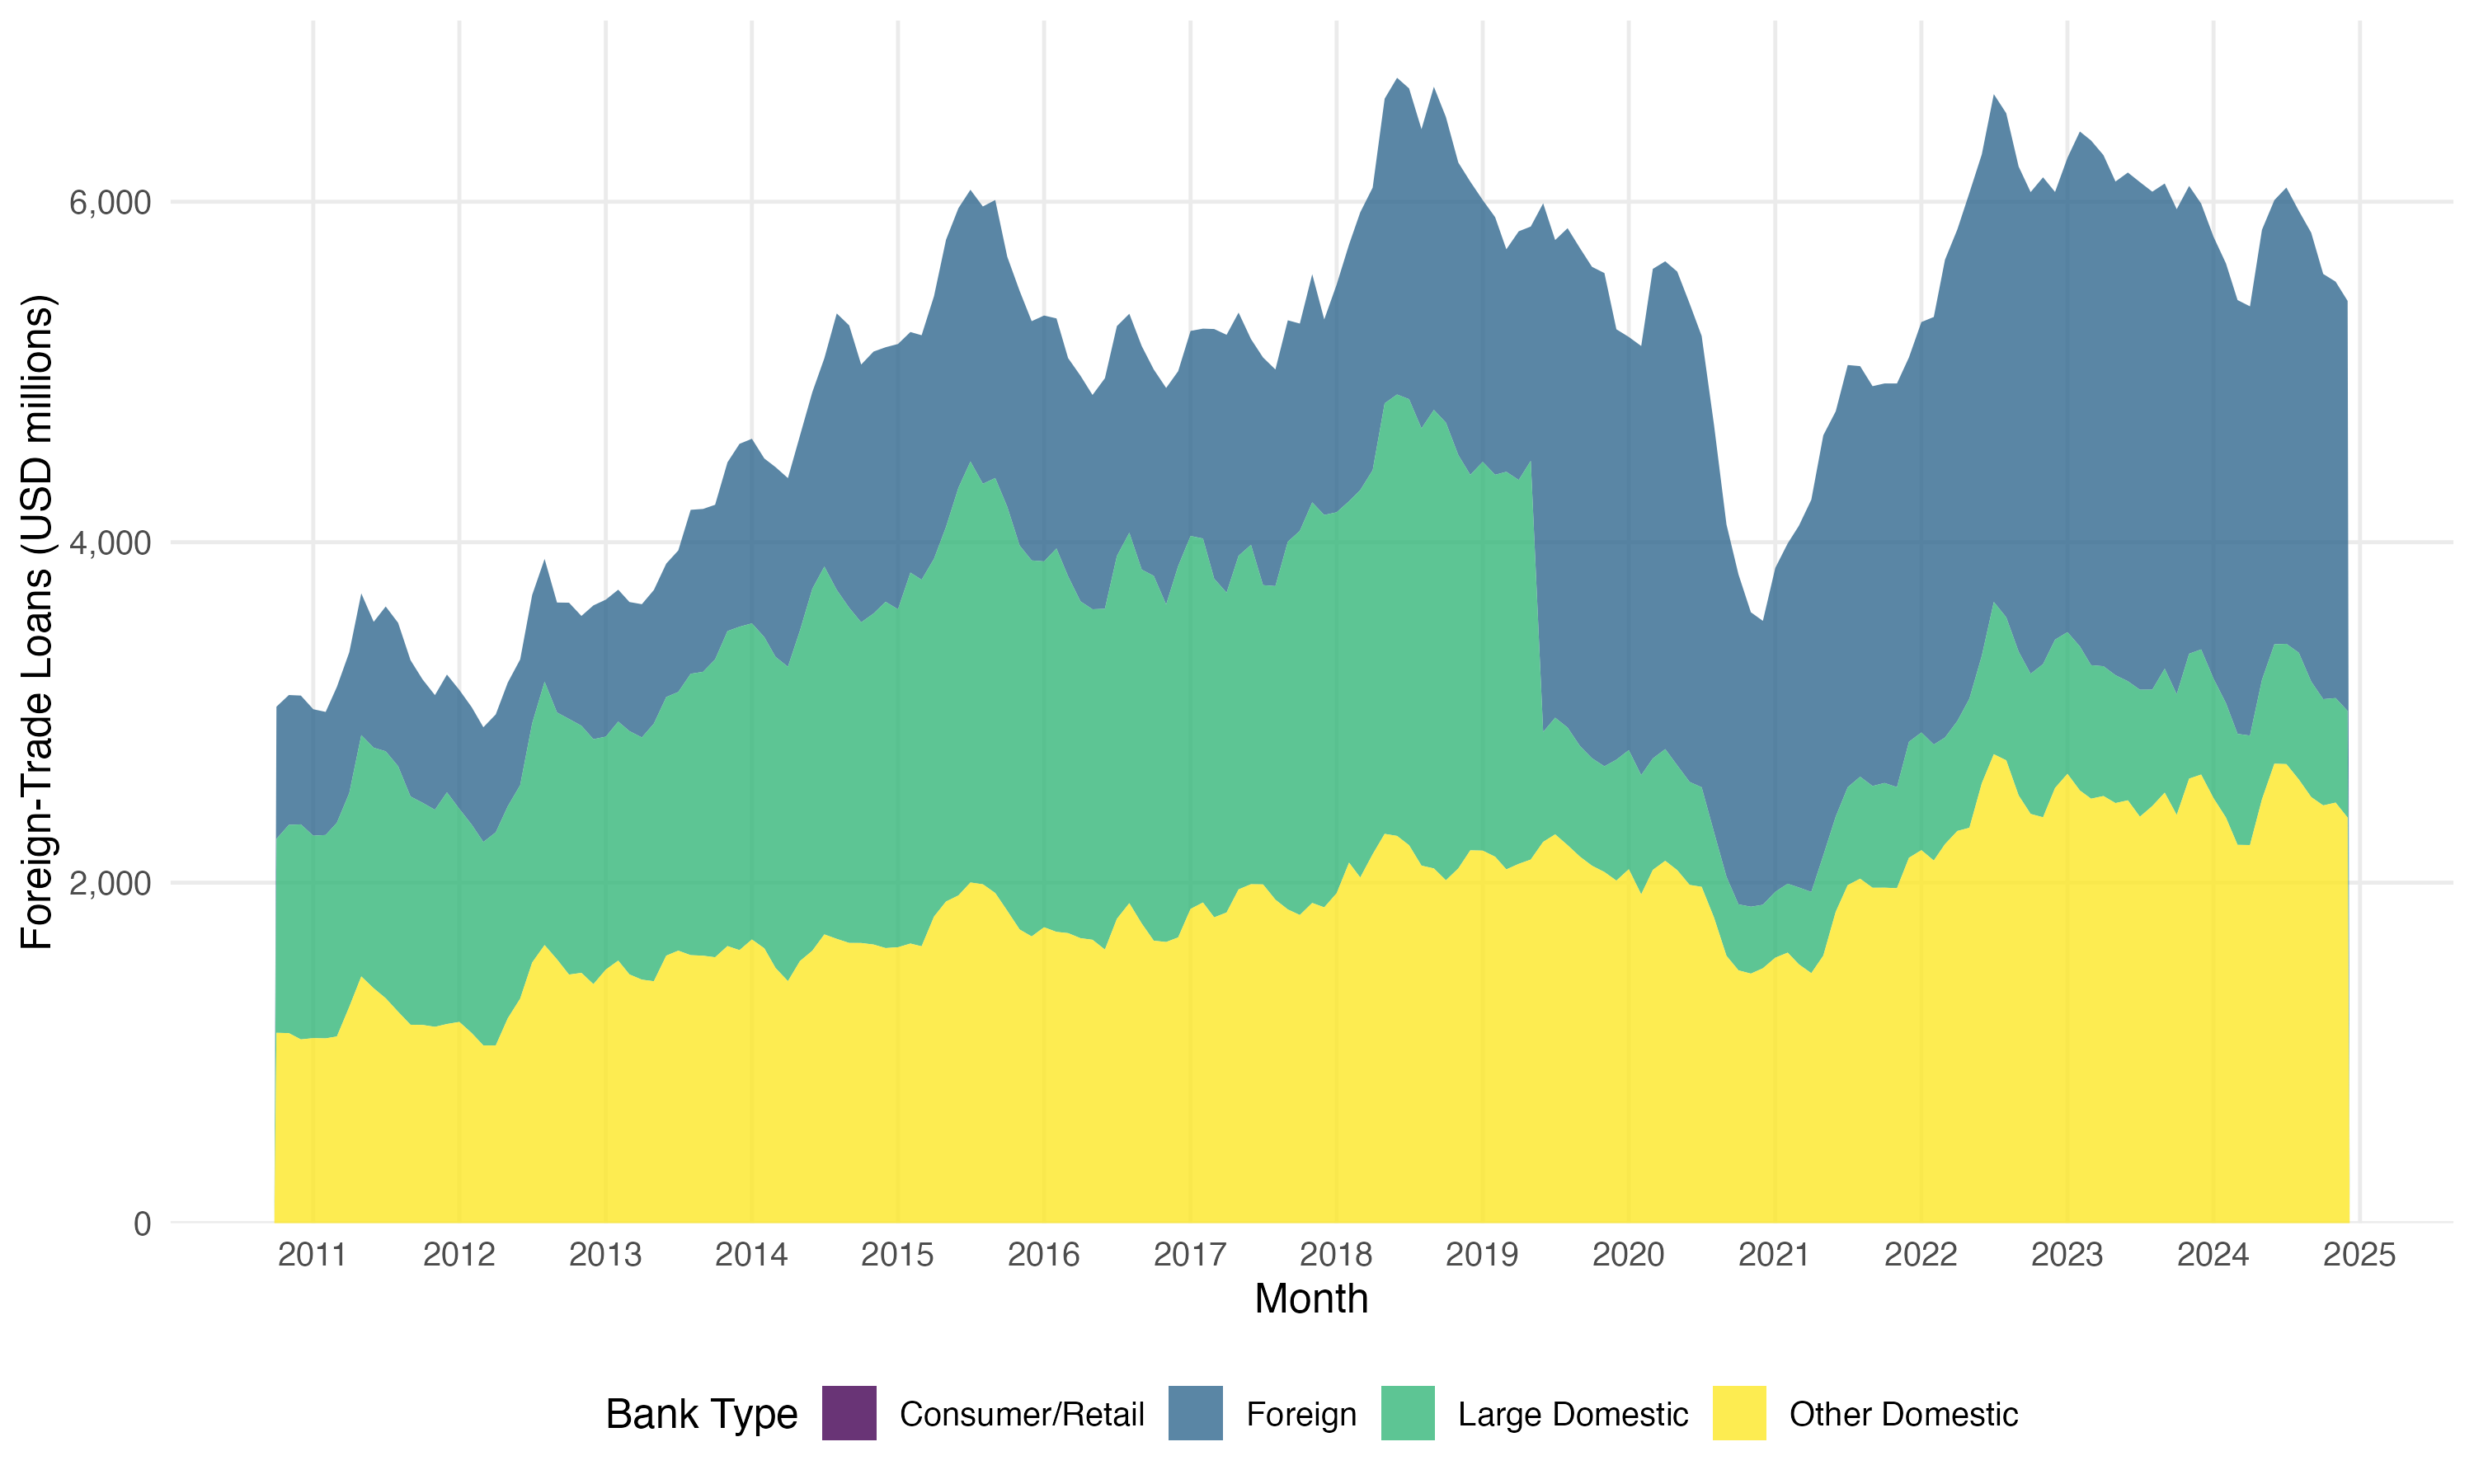
\includegraphics[width=0.7\textwidth]{plots/peru/per_03_tf_by_bank_type.png}
\end{center}
\vspace{-0.3cm}
\small
\textbf{Description:} Monthly stacked area chart showing TF composition by bank type. 2022-2024.

\vspace{0.2cm}
\textbf{Source:} SBS Balance de Comprobación

\vspace{0.2cm}
\textbf{Notes:} Foreign banks: ~35-40\% market share. Includes BBVA, Scotiabank, Citibank.
\end{frame}

\begin{frame}{PER-4: Market Concentration (HHI)}
\begin{center}
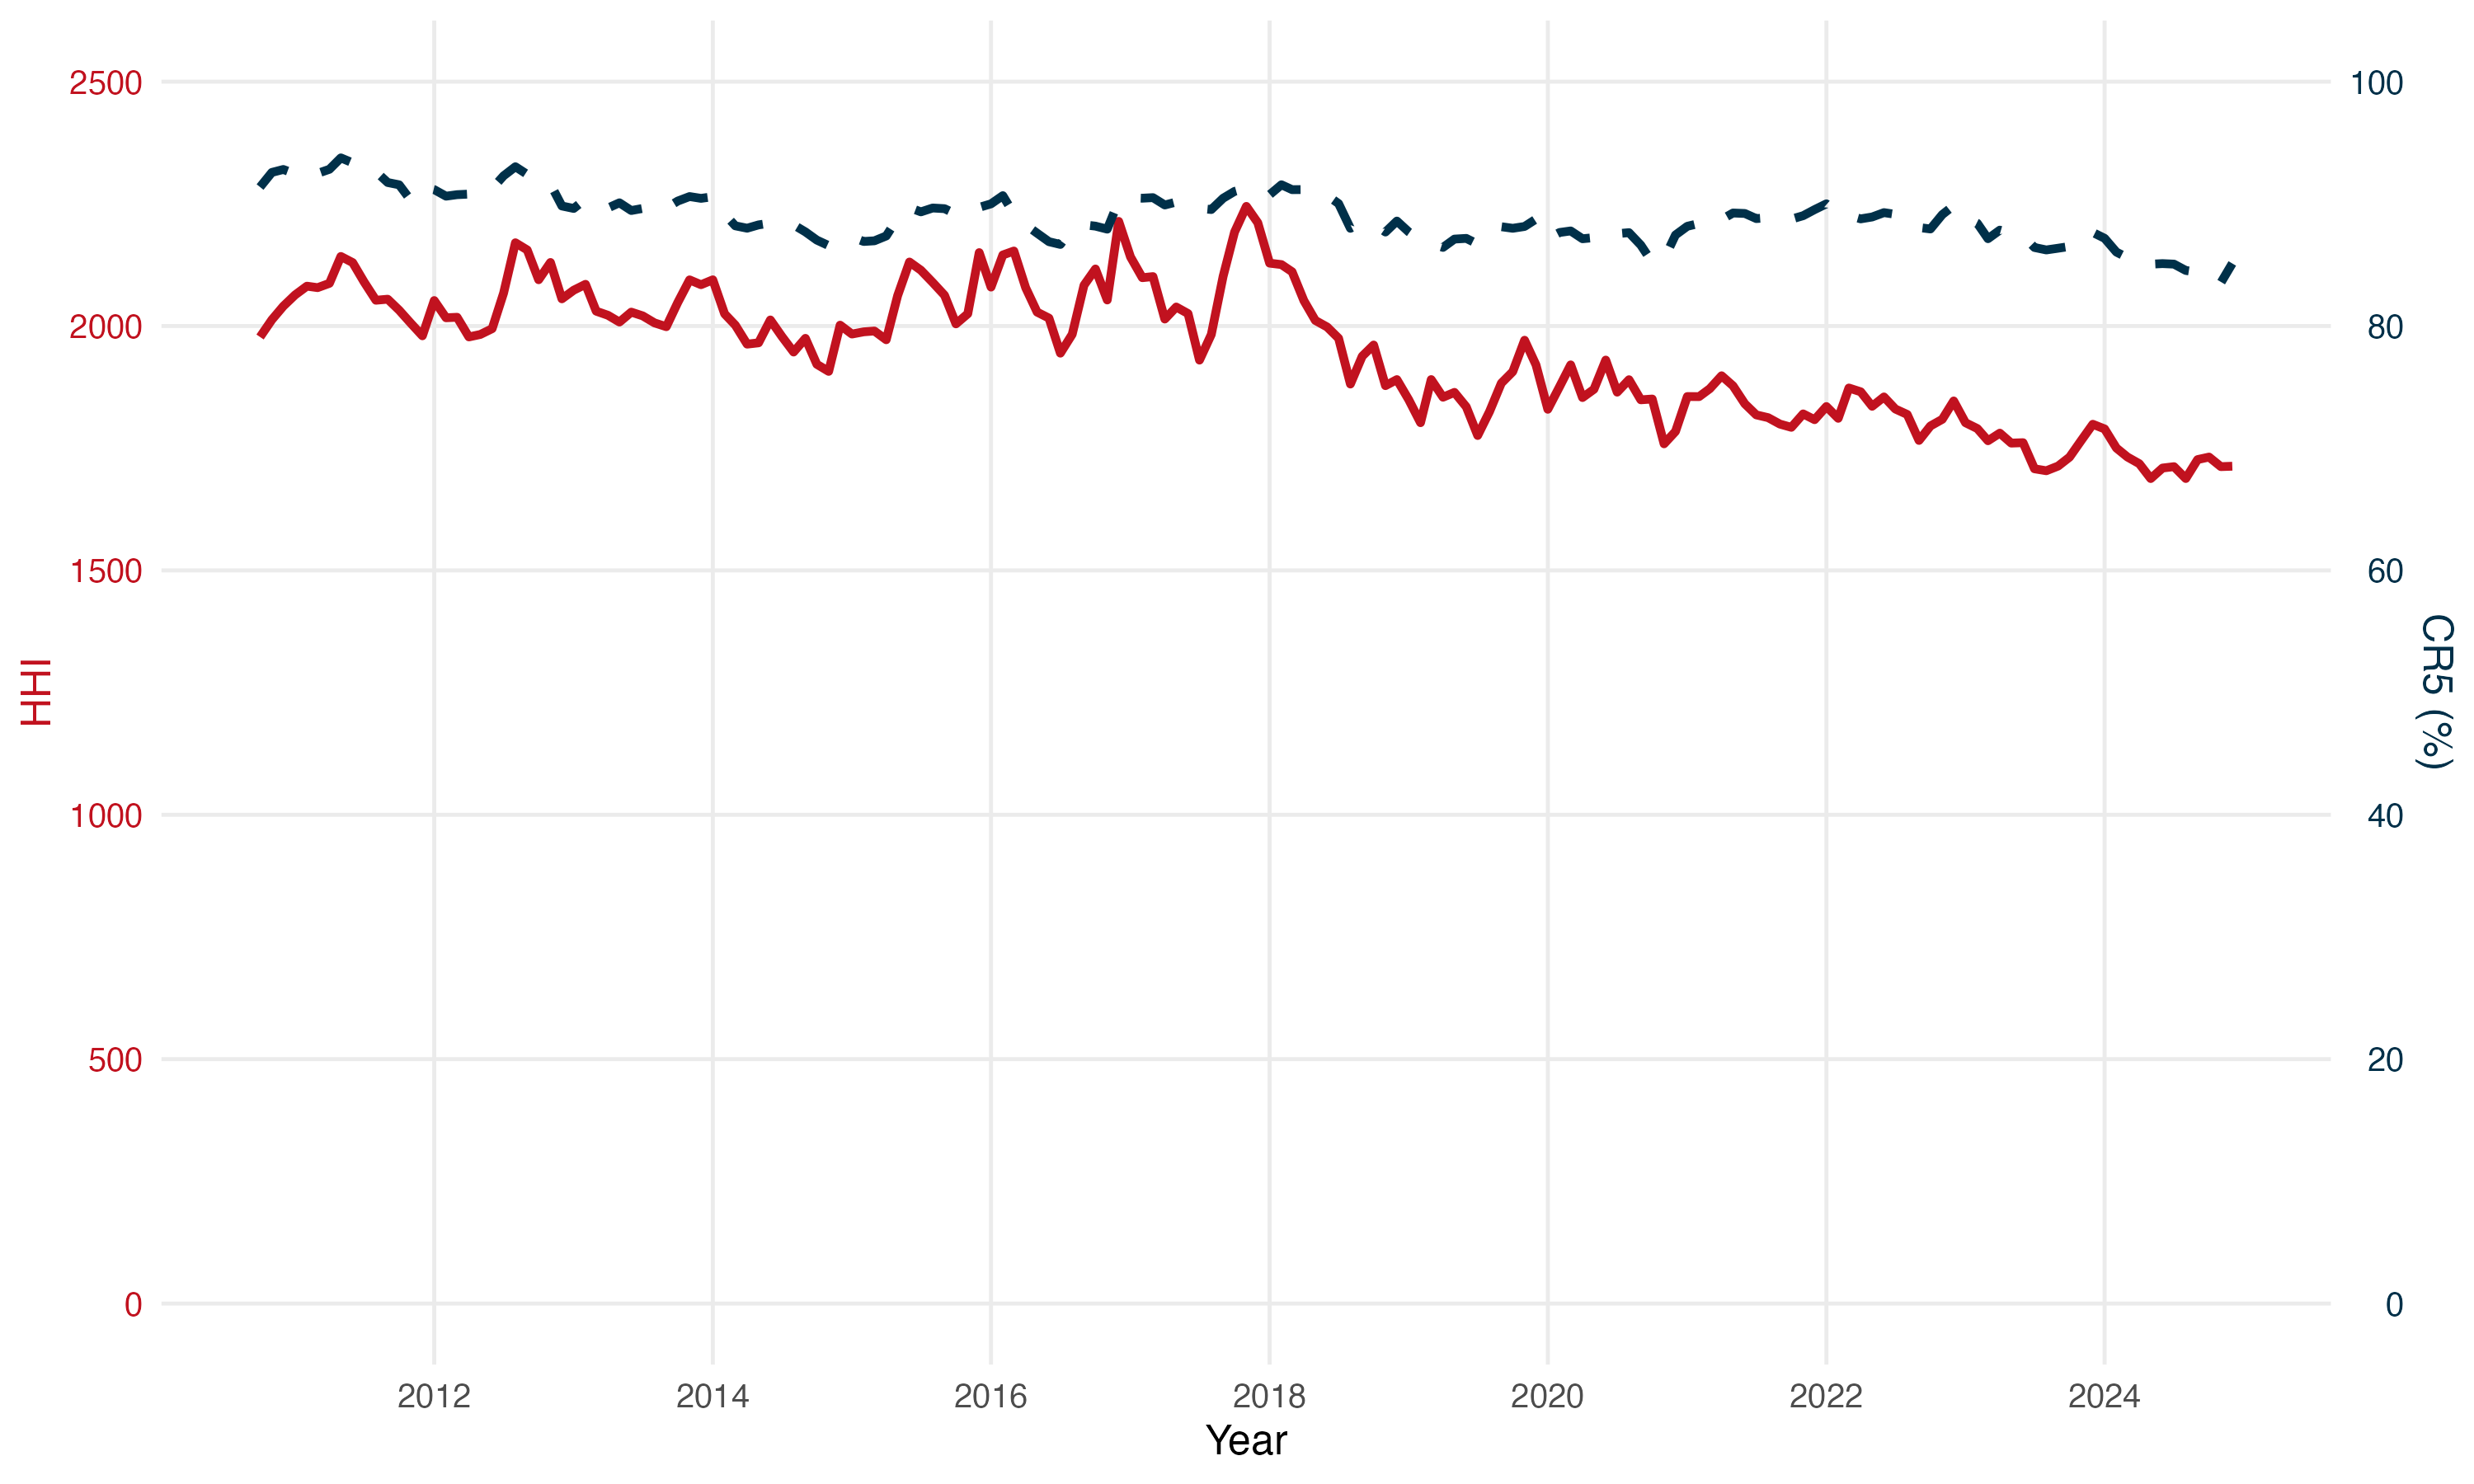
\includegraphics[width=0.7\textwidth]{plots/peru/per_04_concentration.png}
\end{center}
\vspace{-0.3cm}
\small
\textbf{Description:} Herfindahl-Hirschman Index tracking market concentration. 2010-2024.

\vspace{0.2cm}
\textbf{Source:} SBS Balance de Comprobación

\vspace{0.2cm}
\textbf{Notes:} Top 5: BBVA, BCP, Scotiabank, Interbank, Continental. CR5: 75-80\%.
\end{frame}

\begin{frame}{PER-5: TF as \% of Annual Exports}
\begin{center}
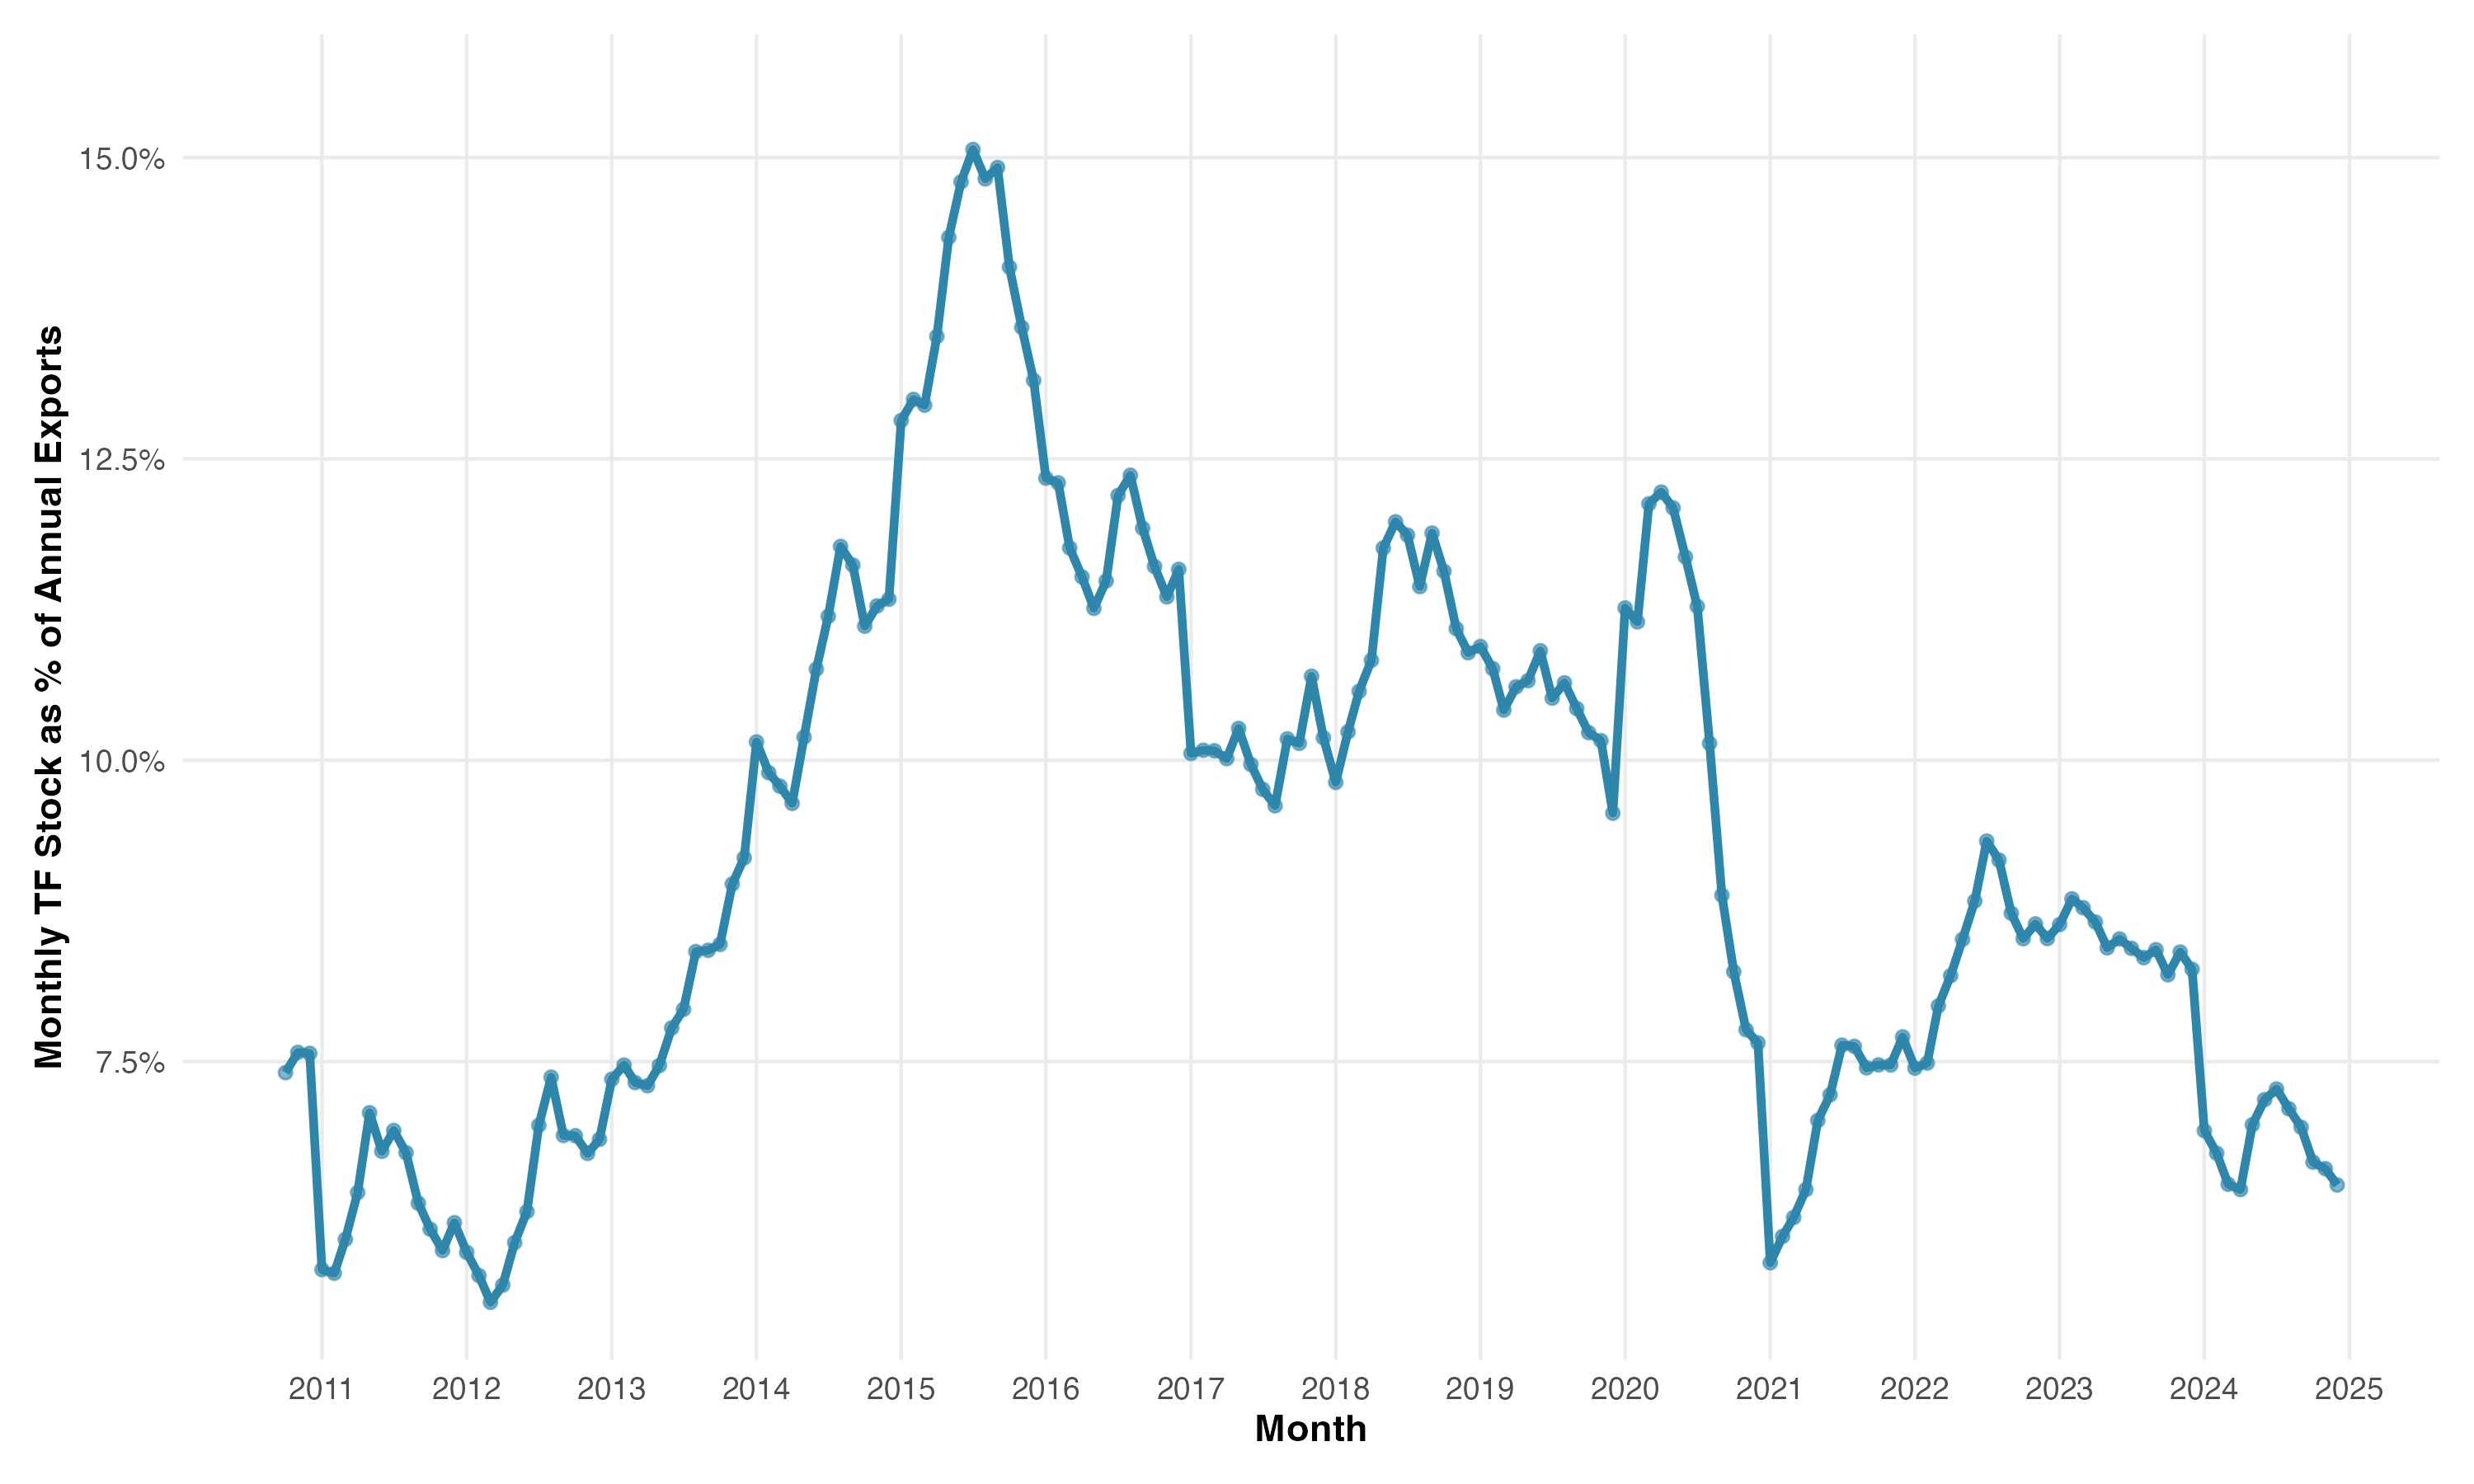
\includegraphics[width=0.7\textwidth]{plots/peru/per_05_tf_pct_exports.png}
\end{center}
\vspace{-0.3cm}
\small
\textbf{Description:} Monthly TF stock as percentage of annual exports. Methodology: monthly stock / annual exports × 100.

\vspace{0.2cm}
\textbf{Source:} SBS Balance de Comprobación + GMD

\vspace{0.2cm}
\textbf{Notes:} Range: 5.5\%-15.1\%.
\end{frame}

\begin{frame}{PER-6: TF as \% of Annual Total Trade}
\begin{center}
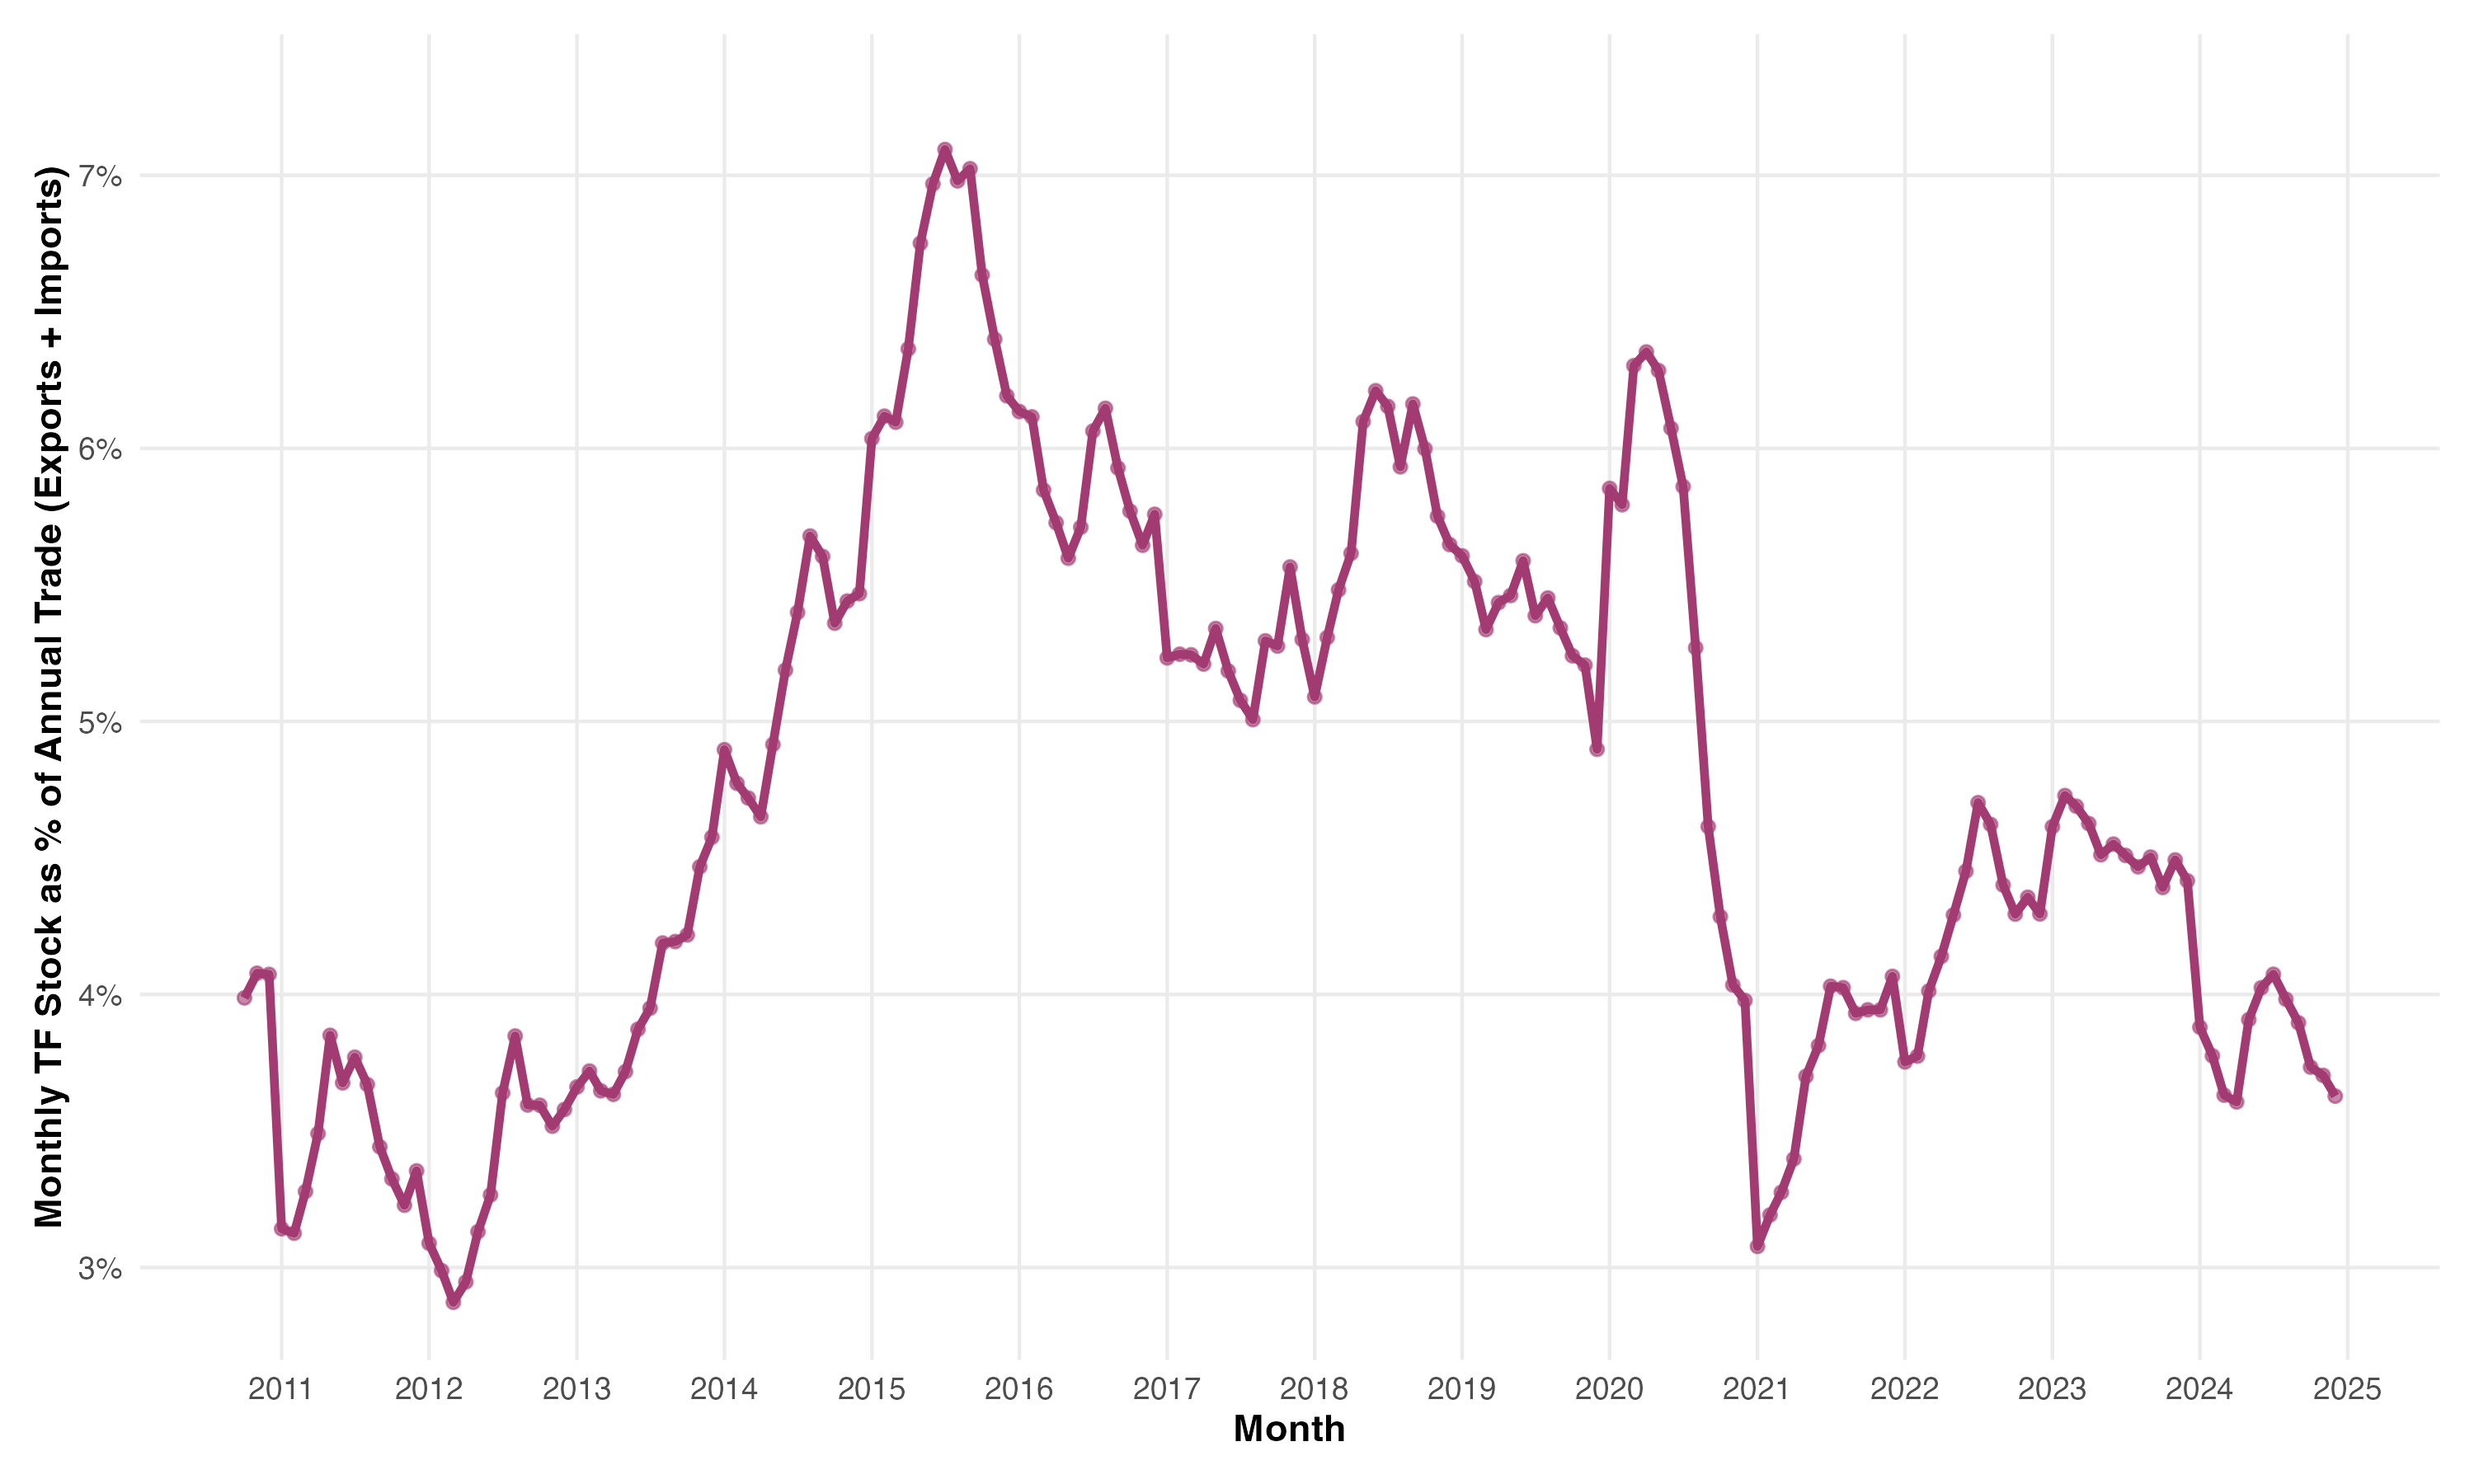
\includegraphics[width=0.7\textwidth]{plots/peru/per_06_tf_pct_trade.png}
\end{center}
\vspace{-0.3cm}
\small
\textbf{Description:} Monthly TF stock as percentage of annual total trade (exports + imports).

\vspace{0.2cm}
\textbf{Source:} SBS Balance de Comprobación + GMD

\vspace{0.2cm}
\textbf{Notes:} Range: 2.9\%-7.1\%.
\end{frame}

\begin{frame}{PER-7: TF by Top 5 Banks (Monthly)}
\begin{center}
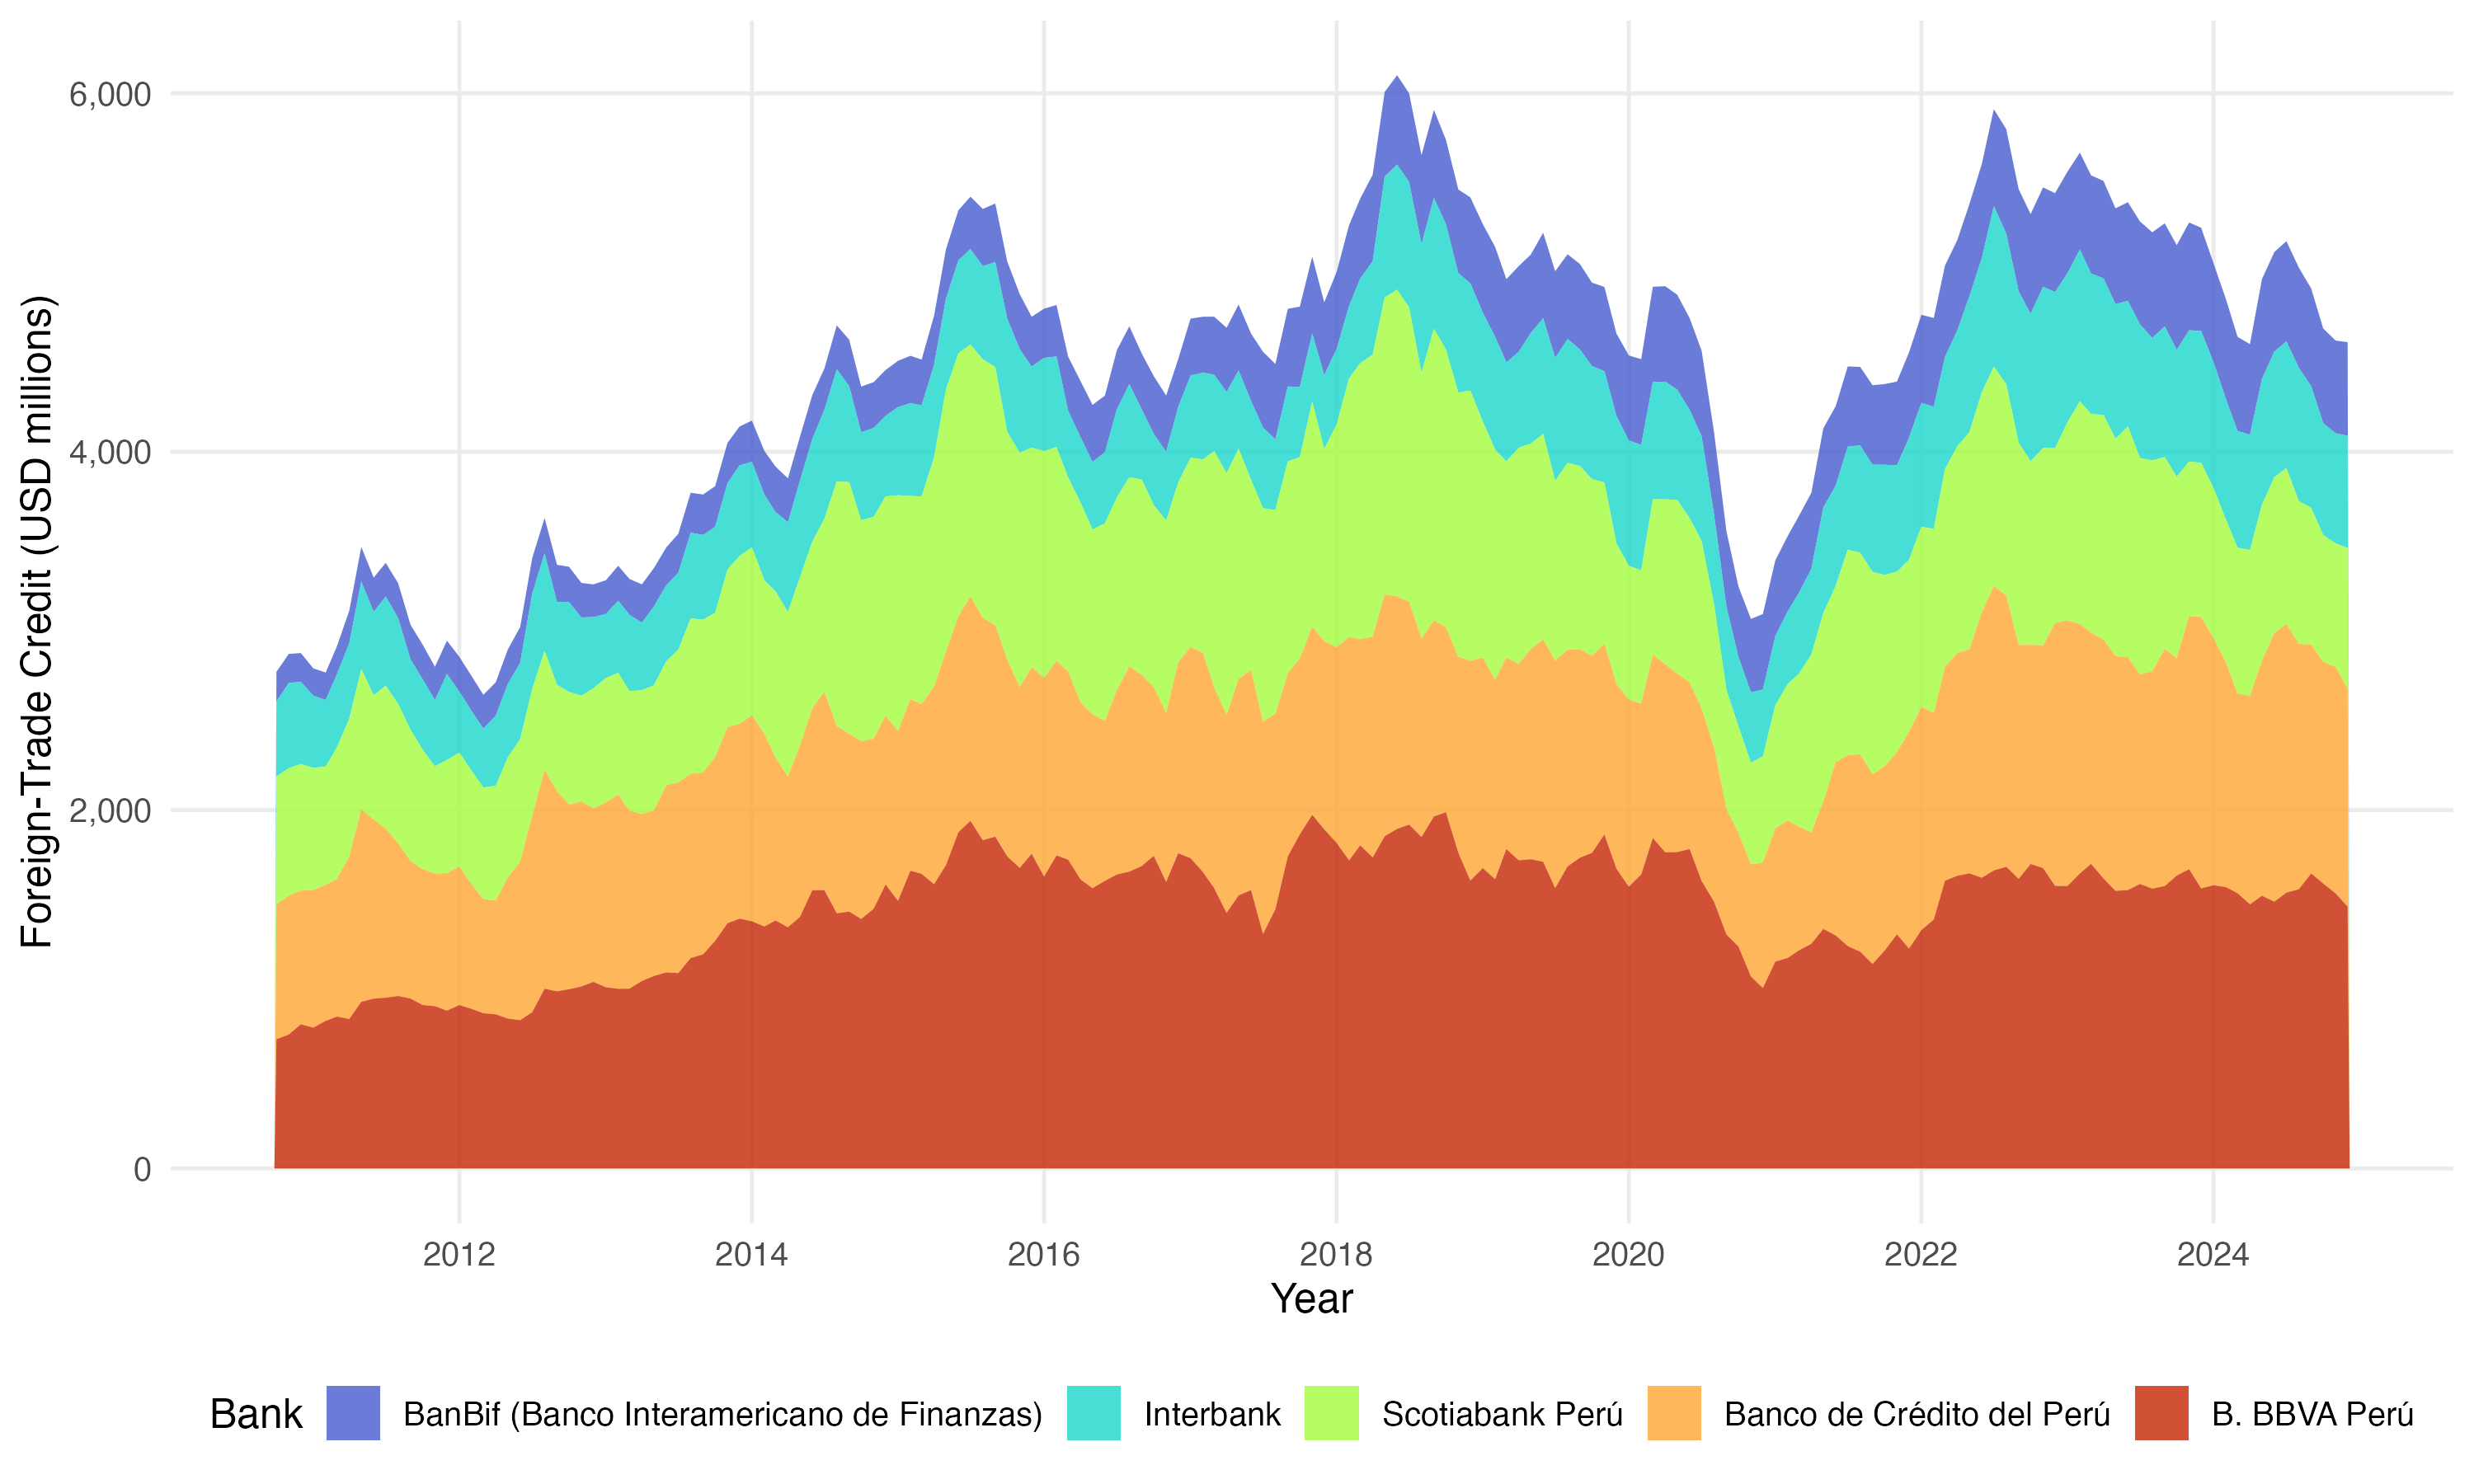
\includegraphics[width=0.7\textwidth]{plots/peru/per_07_tf_top5_banks.png}
\end{center}
\vspace{-0.3cm}
\small
\textbf{Description:} Monthly stacked area showing foreign-trade credit concentration among top 5 institutions. 2010-2024.

\vspace{0.2cm}
\textbf{Source:} SBS Balance de Comprobación

\vspace{0.2cm}
\textbf{Notes:} CR5: 75-80\%.
\end{frame}

% ==============================================================================
% SECTION 4: CHILE GRAPHS
% ==============================================================================

\section{Chile}

% Country separator slide
\begin{frame}
\begin{center}
\vspace{2cm}
{\Huge \textbf{CHILE}}

\vspace{0.5cm}
{\Large Trade Finance Analysis}

\vspace{1cm}
\large
9 Graphs | 2022-2024 | CMF API

\vspace{0.3cm}
\normalsize
CMF/IFRS 9 Period (Accounting Break Jan 2022)
\end{center}
\end{frame}

\begin{frame}{CHL-1: Foreign-Trade Loans as \% of Total Loans}
\begin{center}
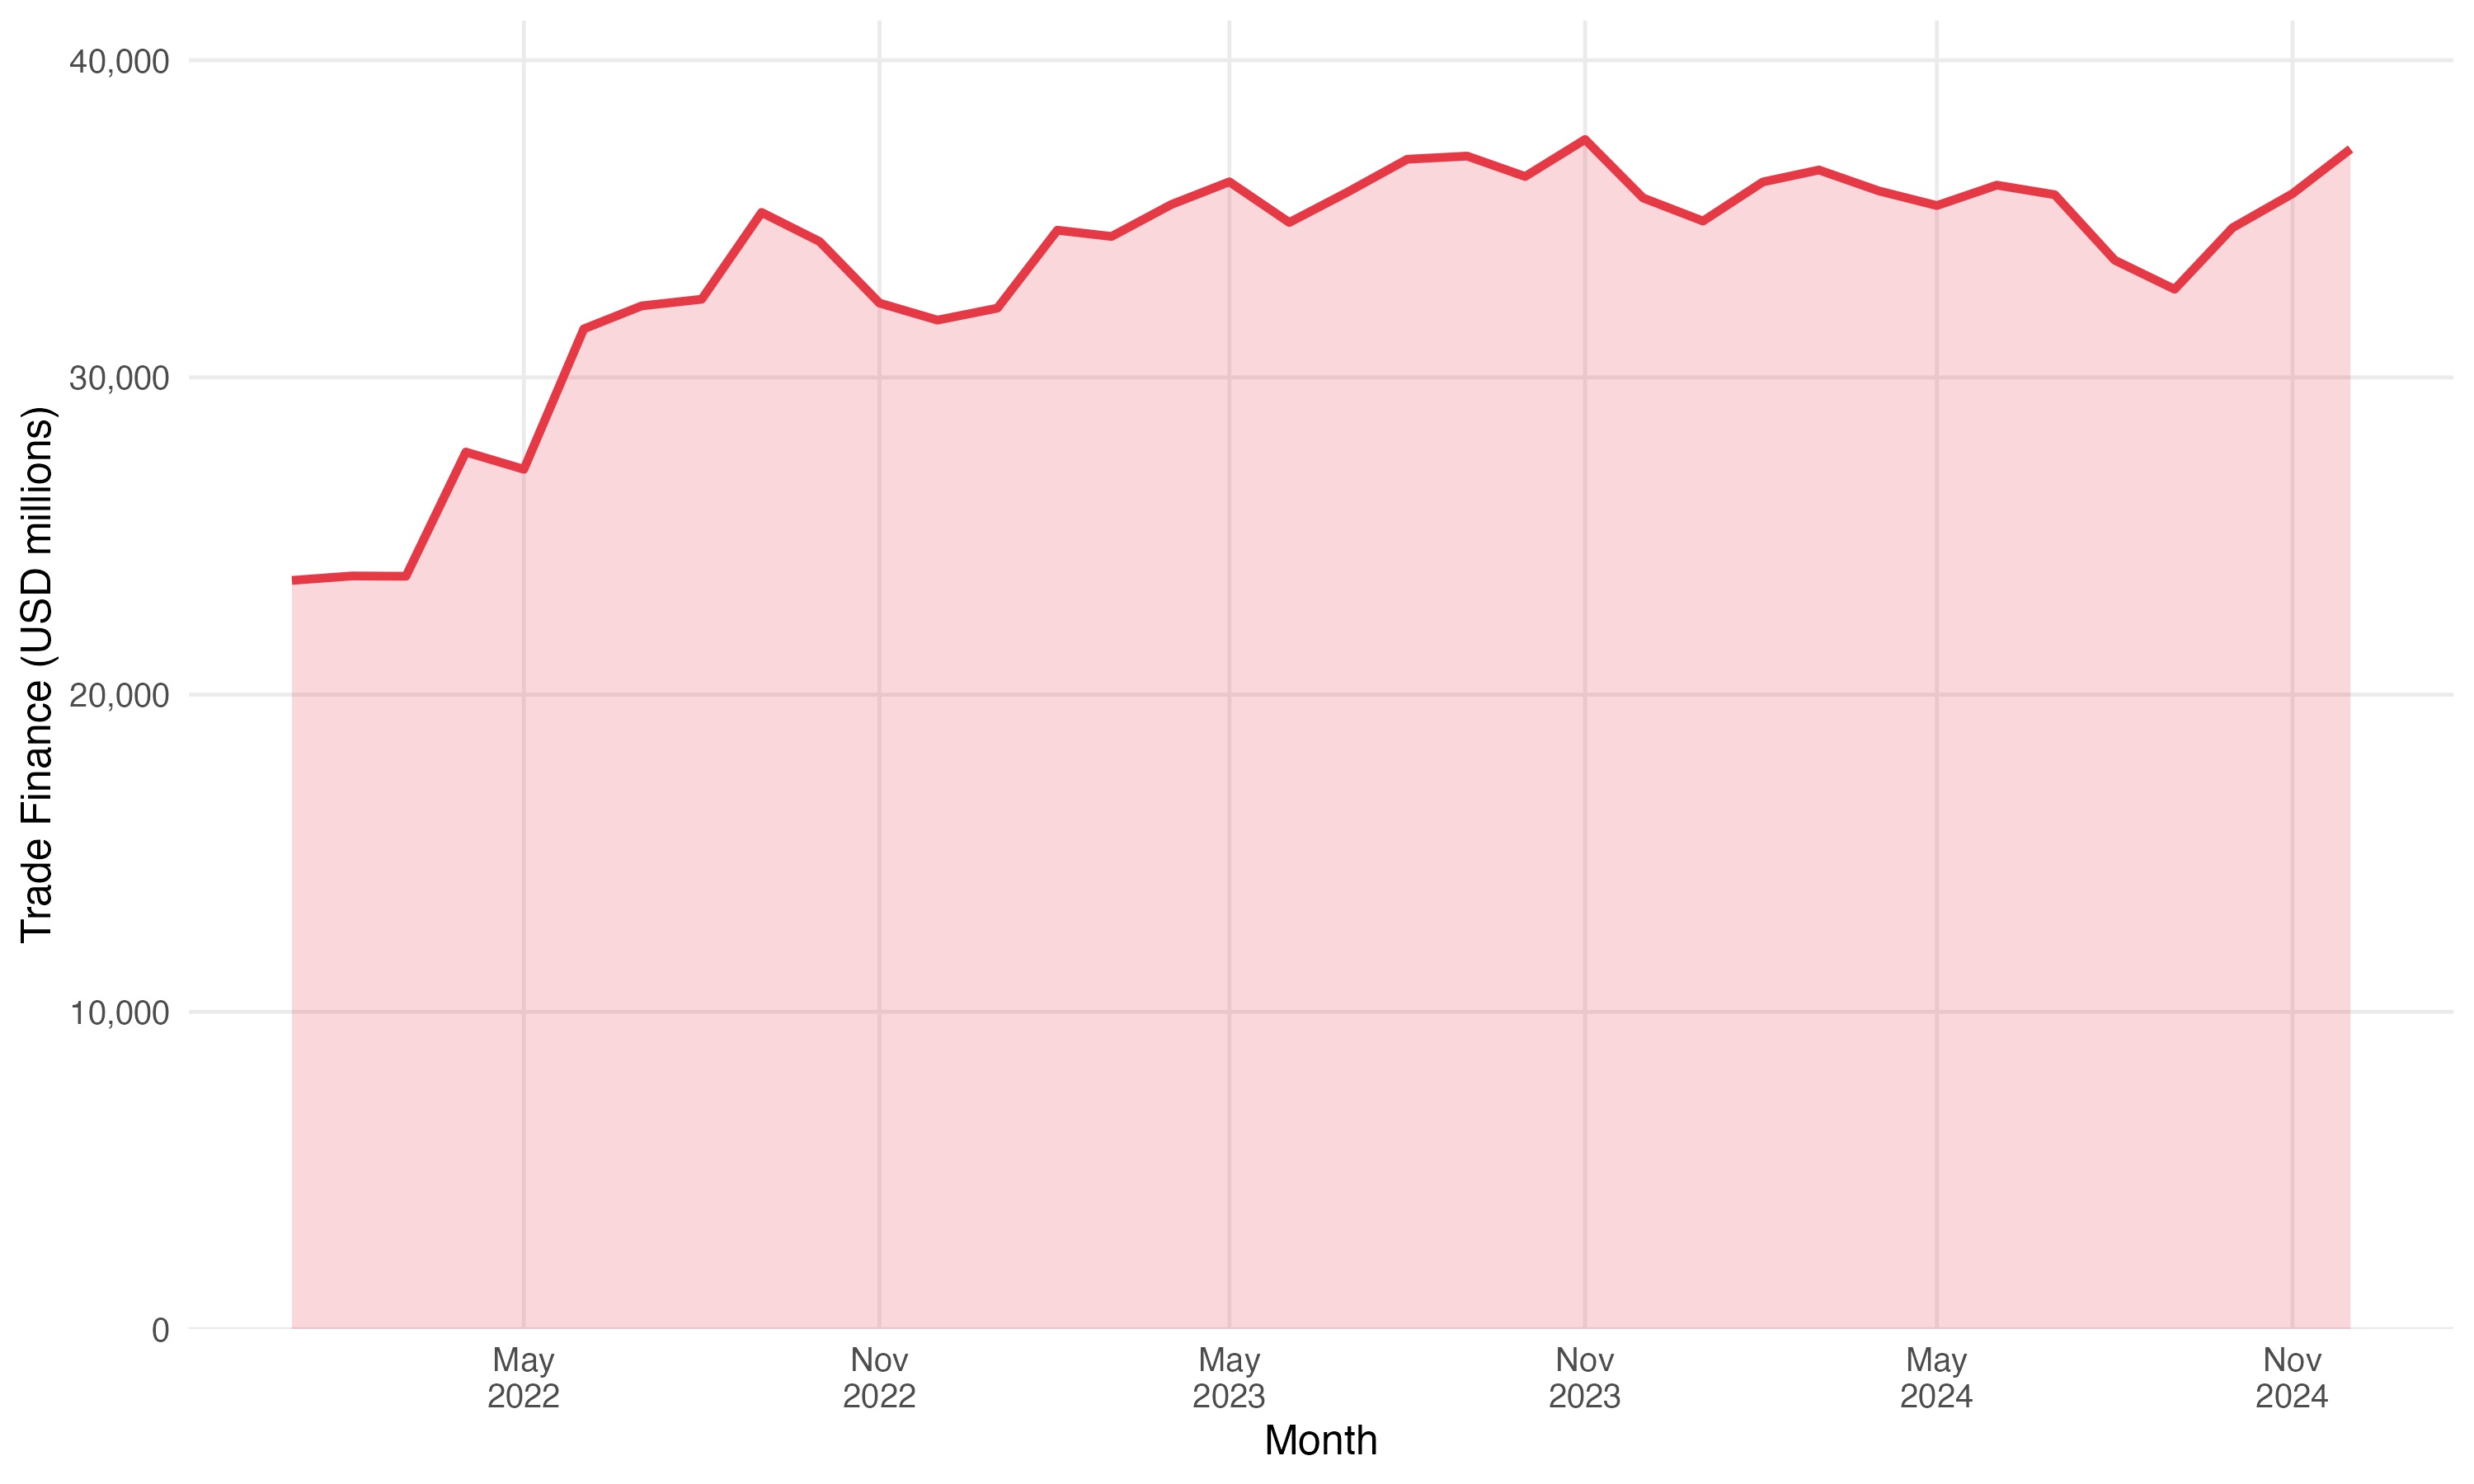
\includegraphics[width=0.7\textwidth]{plots/chile/chl_01_tf_pct_loans.png}
\end{center}
\vspace{-0.3cm}
\small
\textbf{Description:} TF loans as share of total loan portfolio. Series 2015-2024 with SBIF→CMF/IFRS9 accounting transition.

\vspace{0.2cm}
\textbf{Source:} CMF API

\vspace{0.2cm}
\textbf{Notes:} Accounting change January 2022. Jump reflects account identification change (11→29 accounts).
\end{frame}

\begin{frame}{CHL-2: TF by Top 5 Banks (Monthly)}
\begin{center}
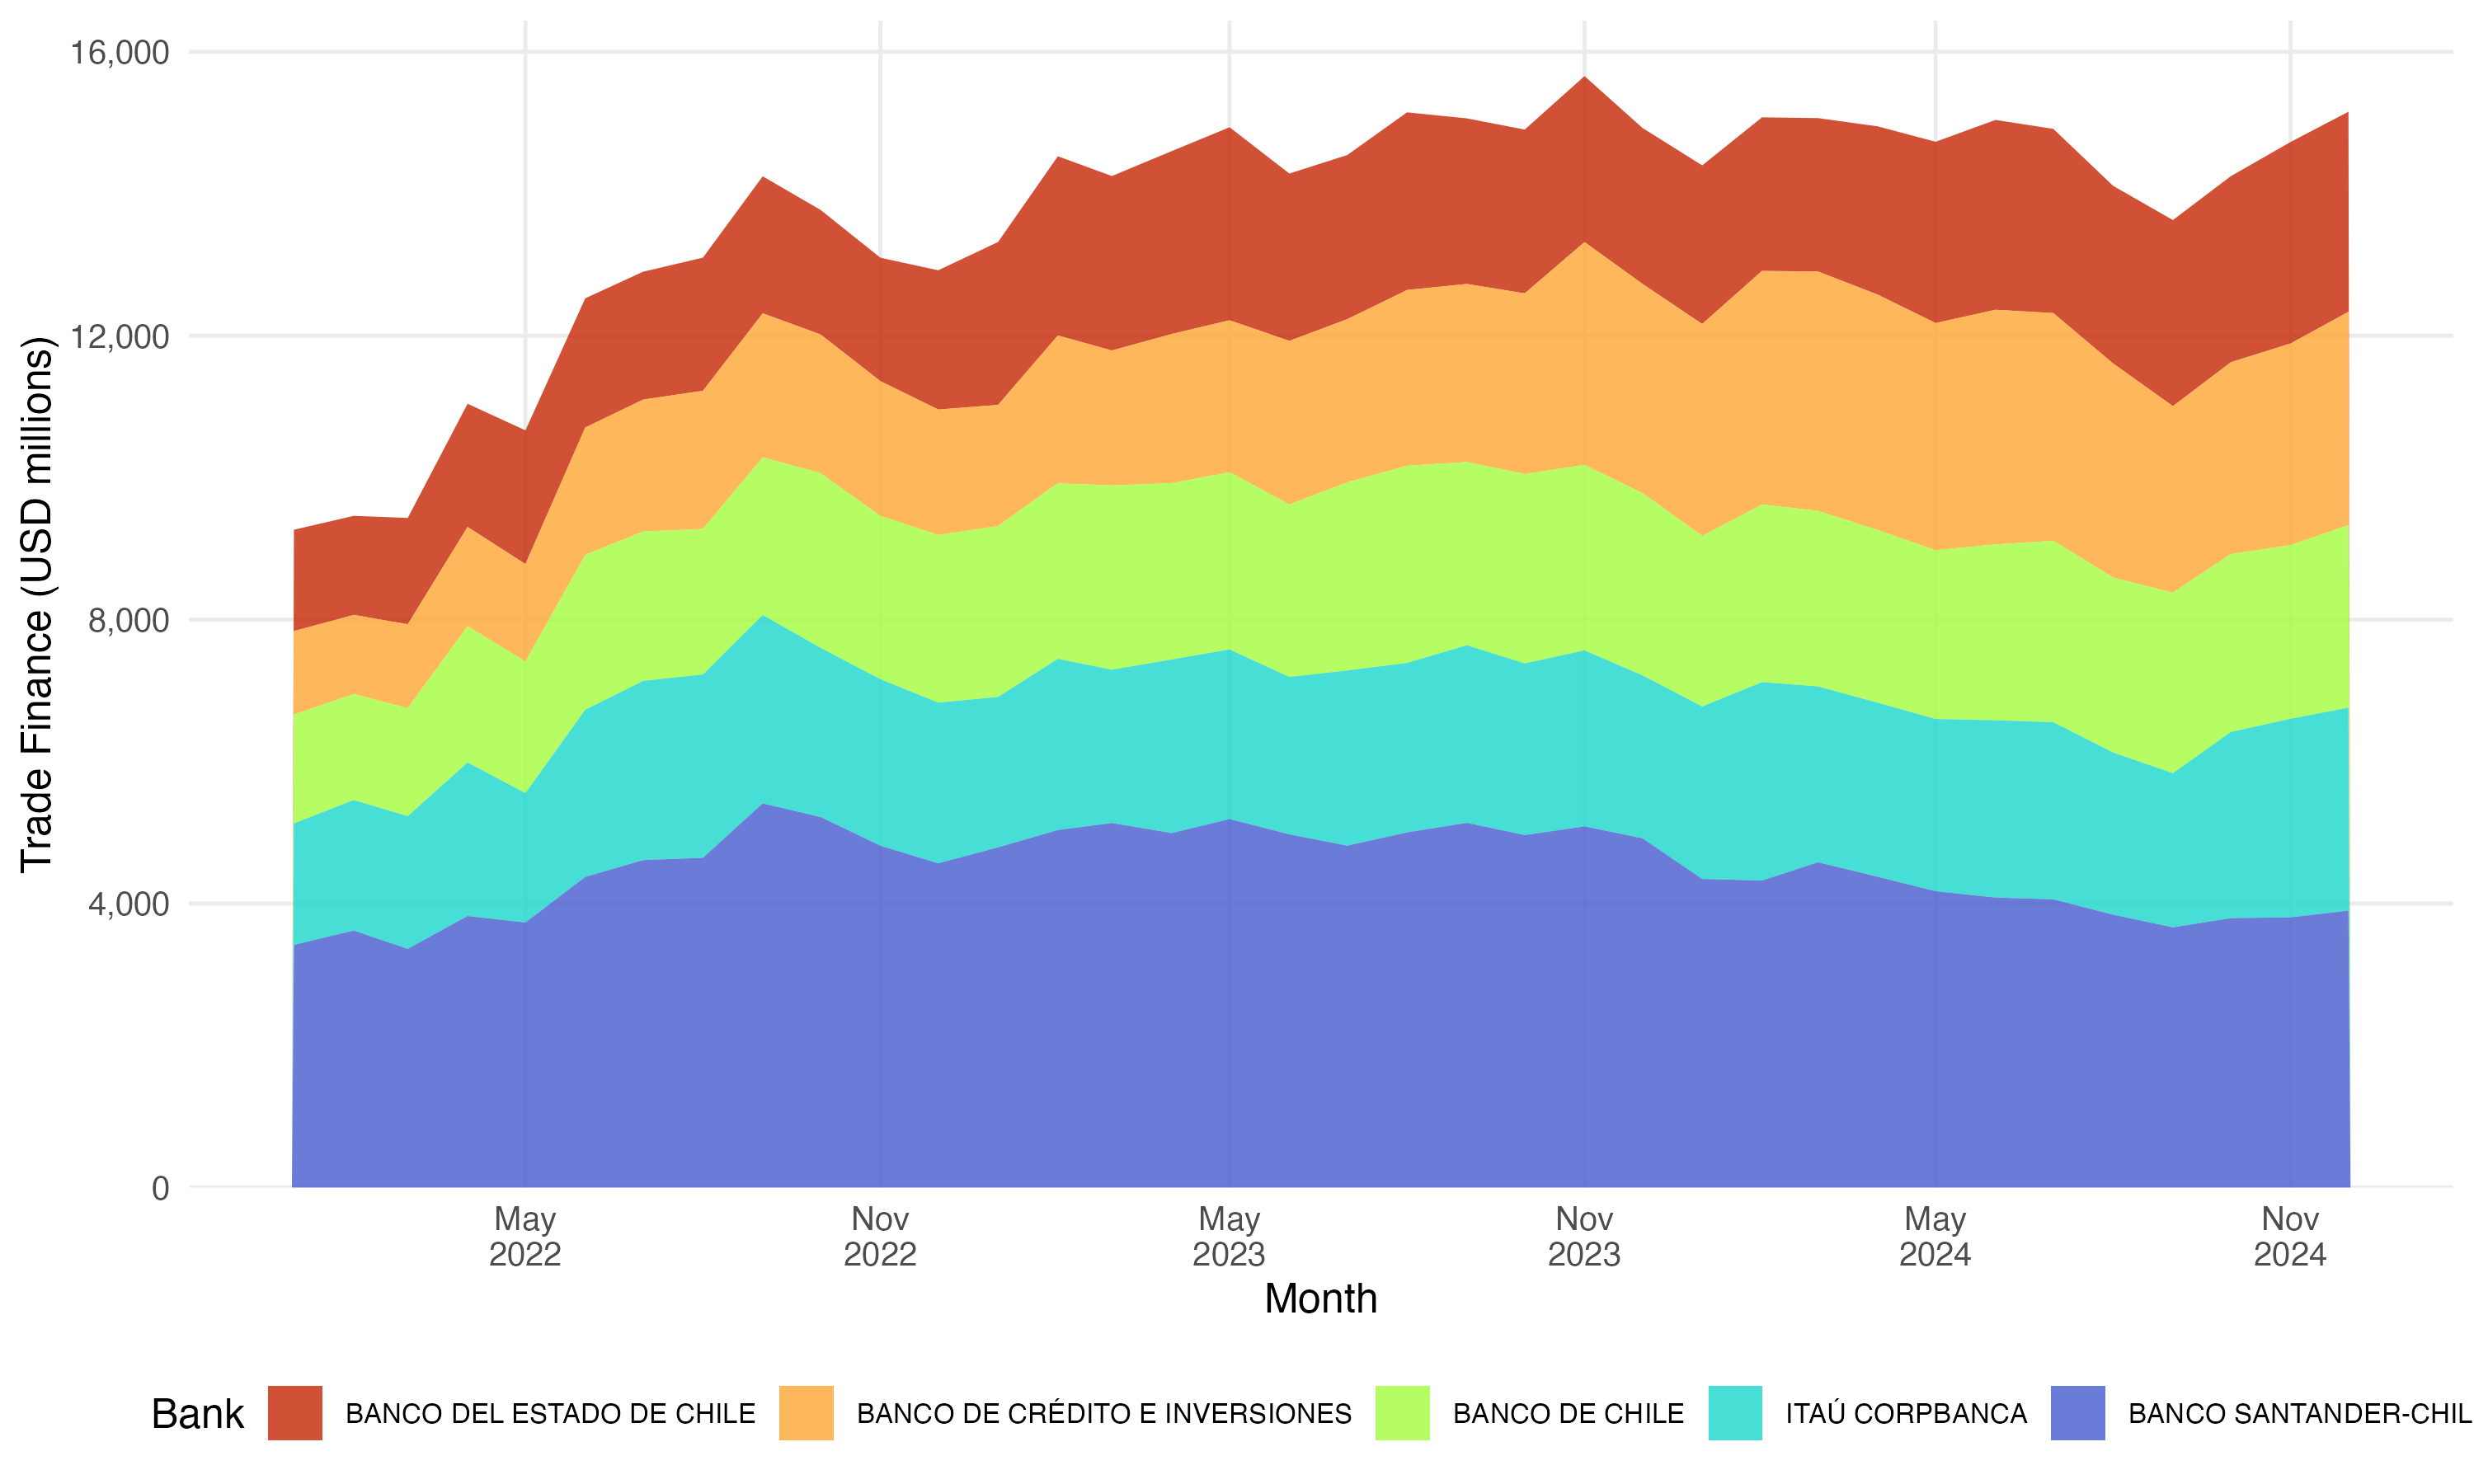
\includegraphics[width=0.7\textwidth]{plots/chile/chl_02_tf_top5_banks.png}
\end{center}
\vspace{-0.3cm}
\small
\textbf{Description:} Monthly stacked area showing TF distribution among top 5 banks. 2022-2024.

\vspace{0.2cm}
\textbf{Source:} CMF API

\vspace{0.2cm}
\textbf{Notes:} Top 5 banks account for majority of TF market.
\end{frame}

\begin{frame}{CHL-3: Market Concentration (HHI)}
\begin{center}
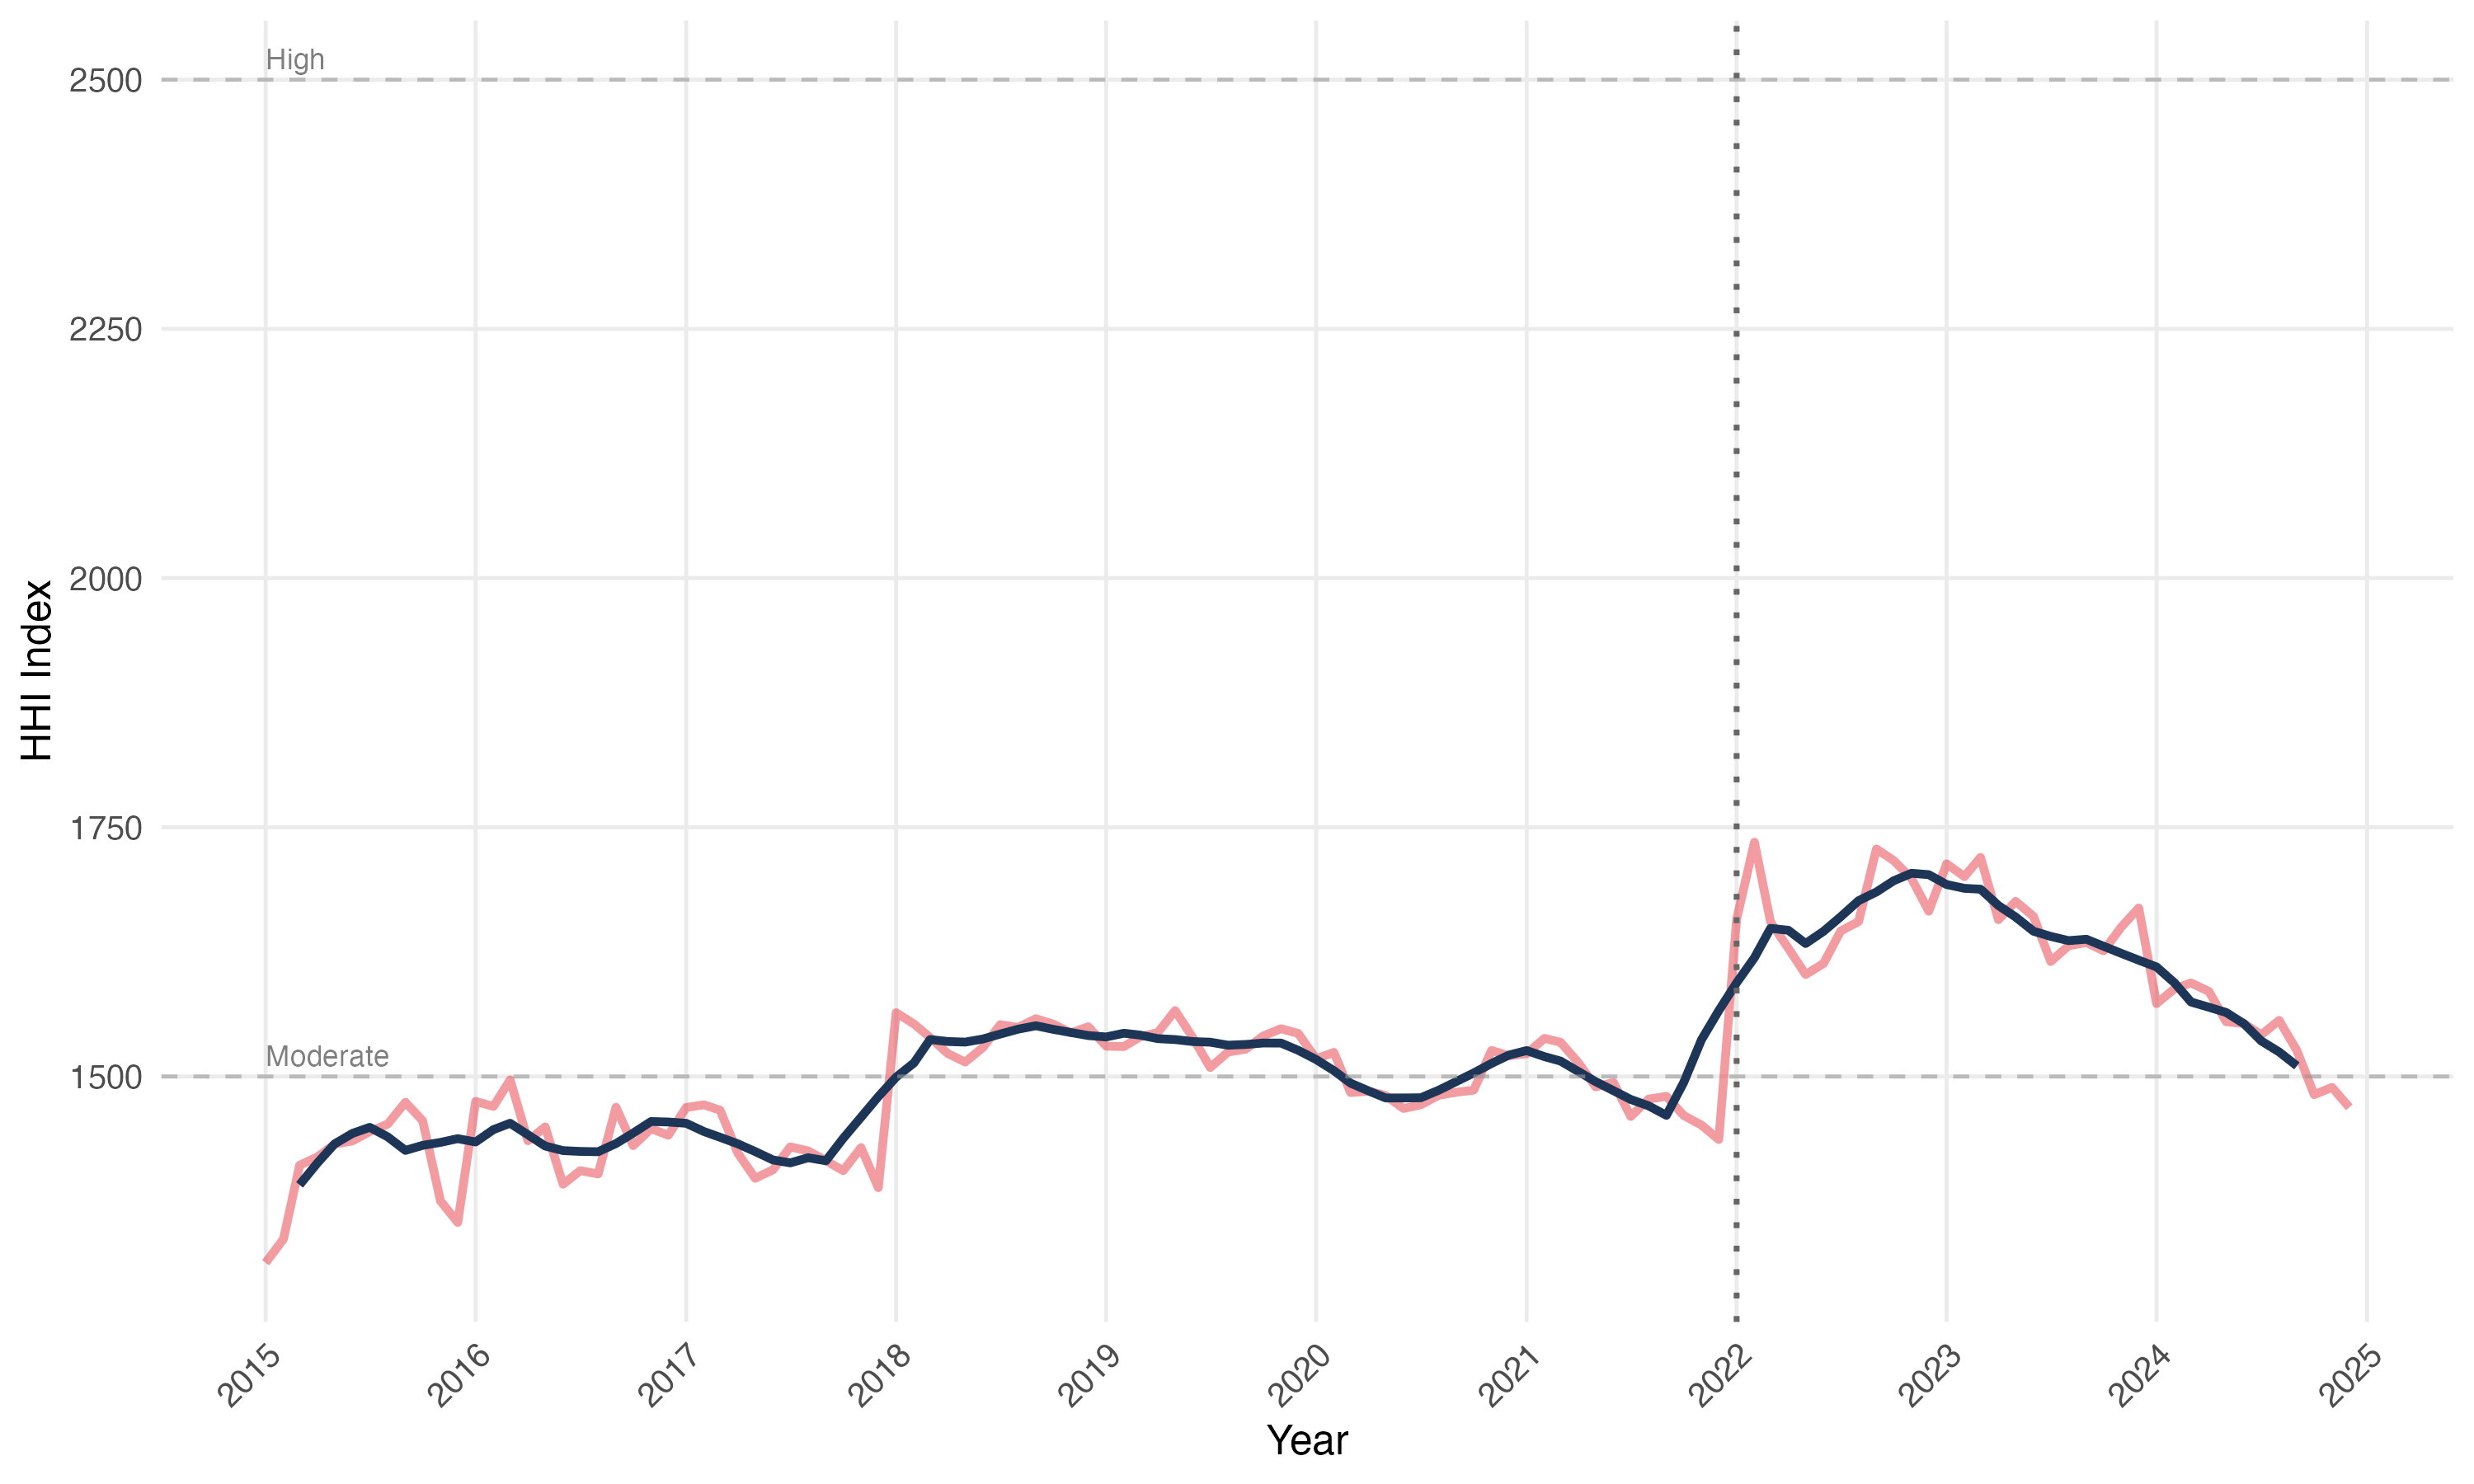
\includegraphics[width=0.7\textwidth]{plots/chile/chl_03_concentration.png}
\end{center}
\vspace{-0.3cm}
\small
\textbf{Description:} Herfindahl-Hirschman Index tracking market concentration 2015-2024.

\vspace{0.2cm}
\textbf{Source:} CMF API

\vspace{0.2cm}
\textbf{Notes:} HHI range: 1313-1735 (moderate concentration).
\end{frame}

\begin{frame}{CHL-4: Interbank Foreign Funding}
\begin{center}
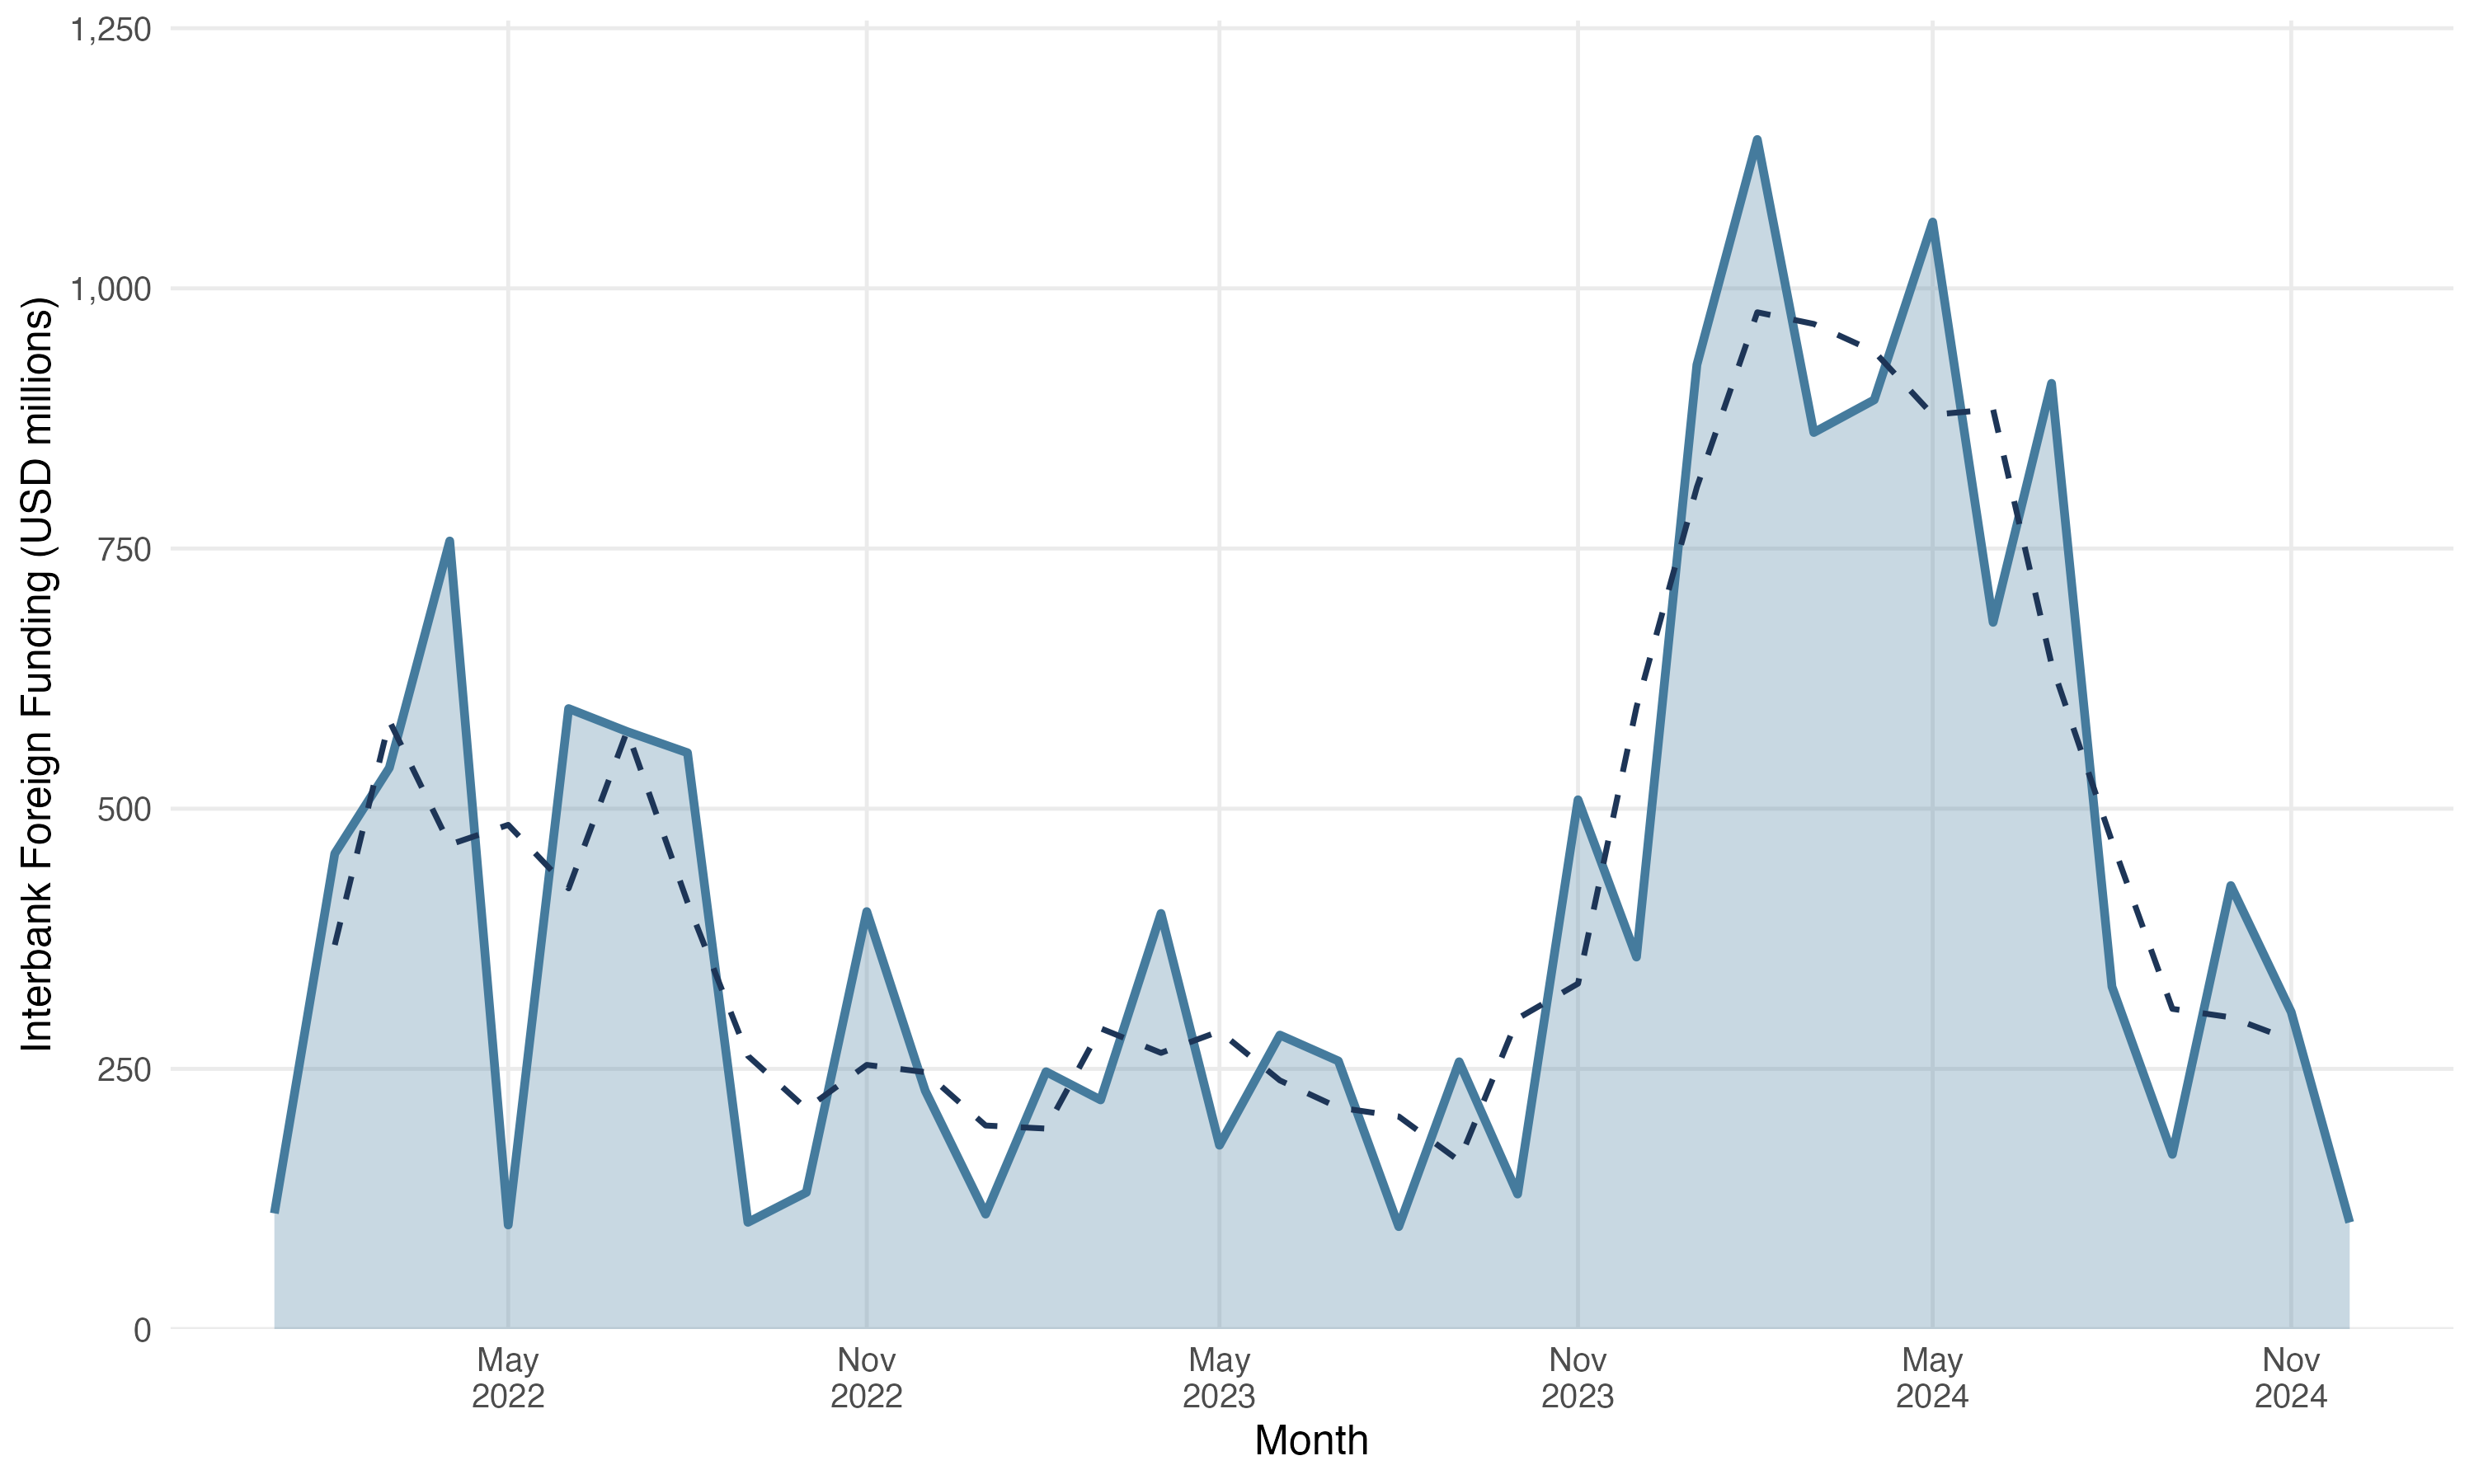
\includegraphics[width=0.7\textwidth]{plots/chile/chl_04_foreign_funding.png}
\end{center}
\vspace{-0.3cm}
\small
\textbf{Description:} Funding from foreign correspondent banks for Chilean trade operations. Monthly 2022-2024.

\vspace{0.2cm}
\textbf{Source:} CMF API

\vspace{0.2cm}
\textbf{Notes:} Range: USD 98-1,143 millions (~1-2\% of total TF).
\end{frame}

\begin{frame}{CHL-5: Letters of Credit as \% of Liabilities}
\begin{center}
\includegraphics[width=0.7\textwidth]{plots/chile/chl_05_lc_pct_liabilities.png}
\end{center}
\vspace{-0.3cm}
\small
\textbf{Description:} Outstanding L/C as percentage of total bank liabilities. Monthly 2022-2024.

\vspace{0.2cm}
\textbf{Source:} CMF API

\vspace{0.2cm}
\textbf{Notes:} Range: 0.081\%-0.116\%.
\end{frame}

\begin{frame}{CHL-6: L/C by Top 5 Banks (Monthly)}
\begin{center}
\includegraphics[width=0.7\textwidth]{plots/chile/chl_06_lc_top5_banks.png}
\end{center}
\vspace{-0.3cm}
\small
\textbf{Description:} Monthly stacked area showing L/C concentration among top 5 issuing banks. 2022-2024.

\vspace{0.2cm}
\textbf{Source:} CMF API

\vspace{0.2cm}
\textbf{Notes:} Top 5 L/C banks include Itaú CorpBanca, Santander, BICE, BCI, Banco del Estado.
\end{frame}

\begin{frame}{CHL-7: TF as \% of Annual Exports}
\begin{center}
\includegraphics[width=0.7\textwidth]{plots/chile/chl_07_tf_pct_exports.png}
\end{center}
\vspace{-0.3cm}
\small
\textbf{Description:} Monthly TF stock as percentage of annual exports. Methodology: monthly stock / annual exports × 100.

\vspace{0.2cm}
\textbf{Source:} CMF API + GMD

\vspace{0.2cm}
\textbf{Notes:} Range: 22.0\%-35.7\%.
\end{frame}

\begin{frame}{CHL-8: TF as \% of Annual Total Trade}
\begin{center}
\includegraphics[width=0.7\textwidth]{plots/chile/chl_08_tf_pct_trade.png}
\end{center}
\vspace{-0.3cm}
\small
\textbf{Description:} Monthly TF stock as percentage of annual total trade. Methodology: monthly stock / annual (X+M) × 100.

\vspace{0.2cm}
\textbf{Source:} CMF API + GMD

\vspace{0.2cm}
\textbf{Notes:} Range: 10.4\%-18.2\%.
\end{frame}

\begin{frame}{CHL-9: Trade Finance Composition by Category}
\begin{center}
\includegraphics[width=0.7\textwidth]{plots/chile/chl_09_tf_composition.png}
\end{center}
\vspace{-0.3cm}
\small
\textbf{Description:} Monthly stacked area showing TF breakdown by category. 2022-2024.

\vspace{0.2cm}
\textbf{Source:} CMF API

\vspace{0.2cm}
\textbf{Notes:} Top 3 categories: Exports (46\%), Guarantees (26\%), Imports (24\%).
\end{frame}

% ==============================================================================
% SECTION 5: BRAZIL GRAPHS
% ==============================================================================

\section{Brazil}

% Country separator slide
\begin{frame}
\begin{center}
\vspace{2cm}
{\Huge \textbf{BRAZIL}}

\vspace{0.5cm}
{\Large Trade Finance Analysis}

\vspace{1cm}
\large
8 Graphs | 2012-2024 | BCB Monthly Reports

\vspace{0.3cm}
\normalsize
Foreign-Trade Credit (No Bank-Level Data)
\end{center}
\end{frame}

\begin{frame}{BRA-1: Foreign-Trade Credit as \% of Total Credit}
\begin{center}
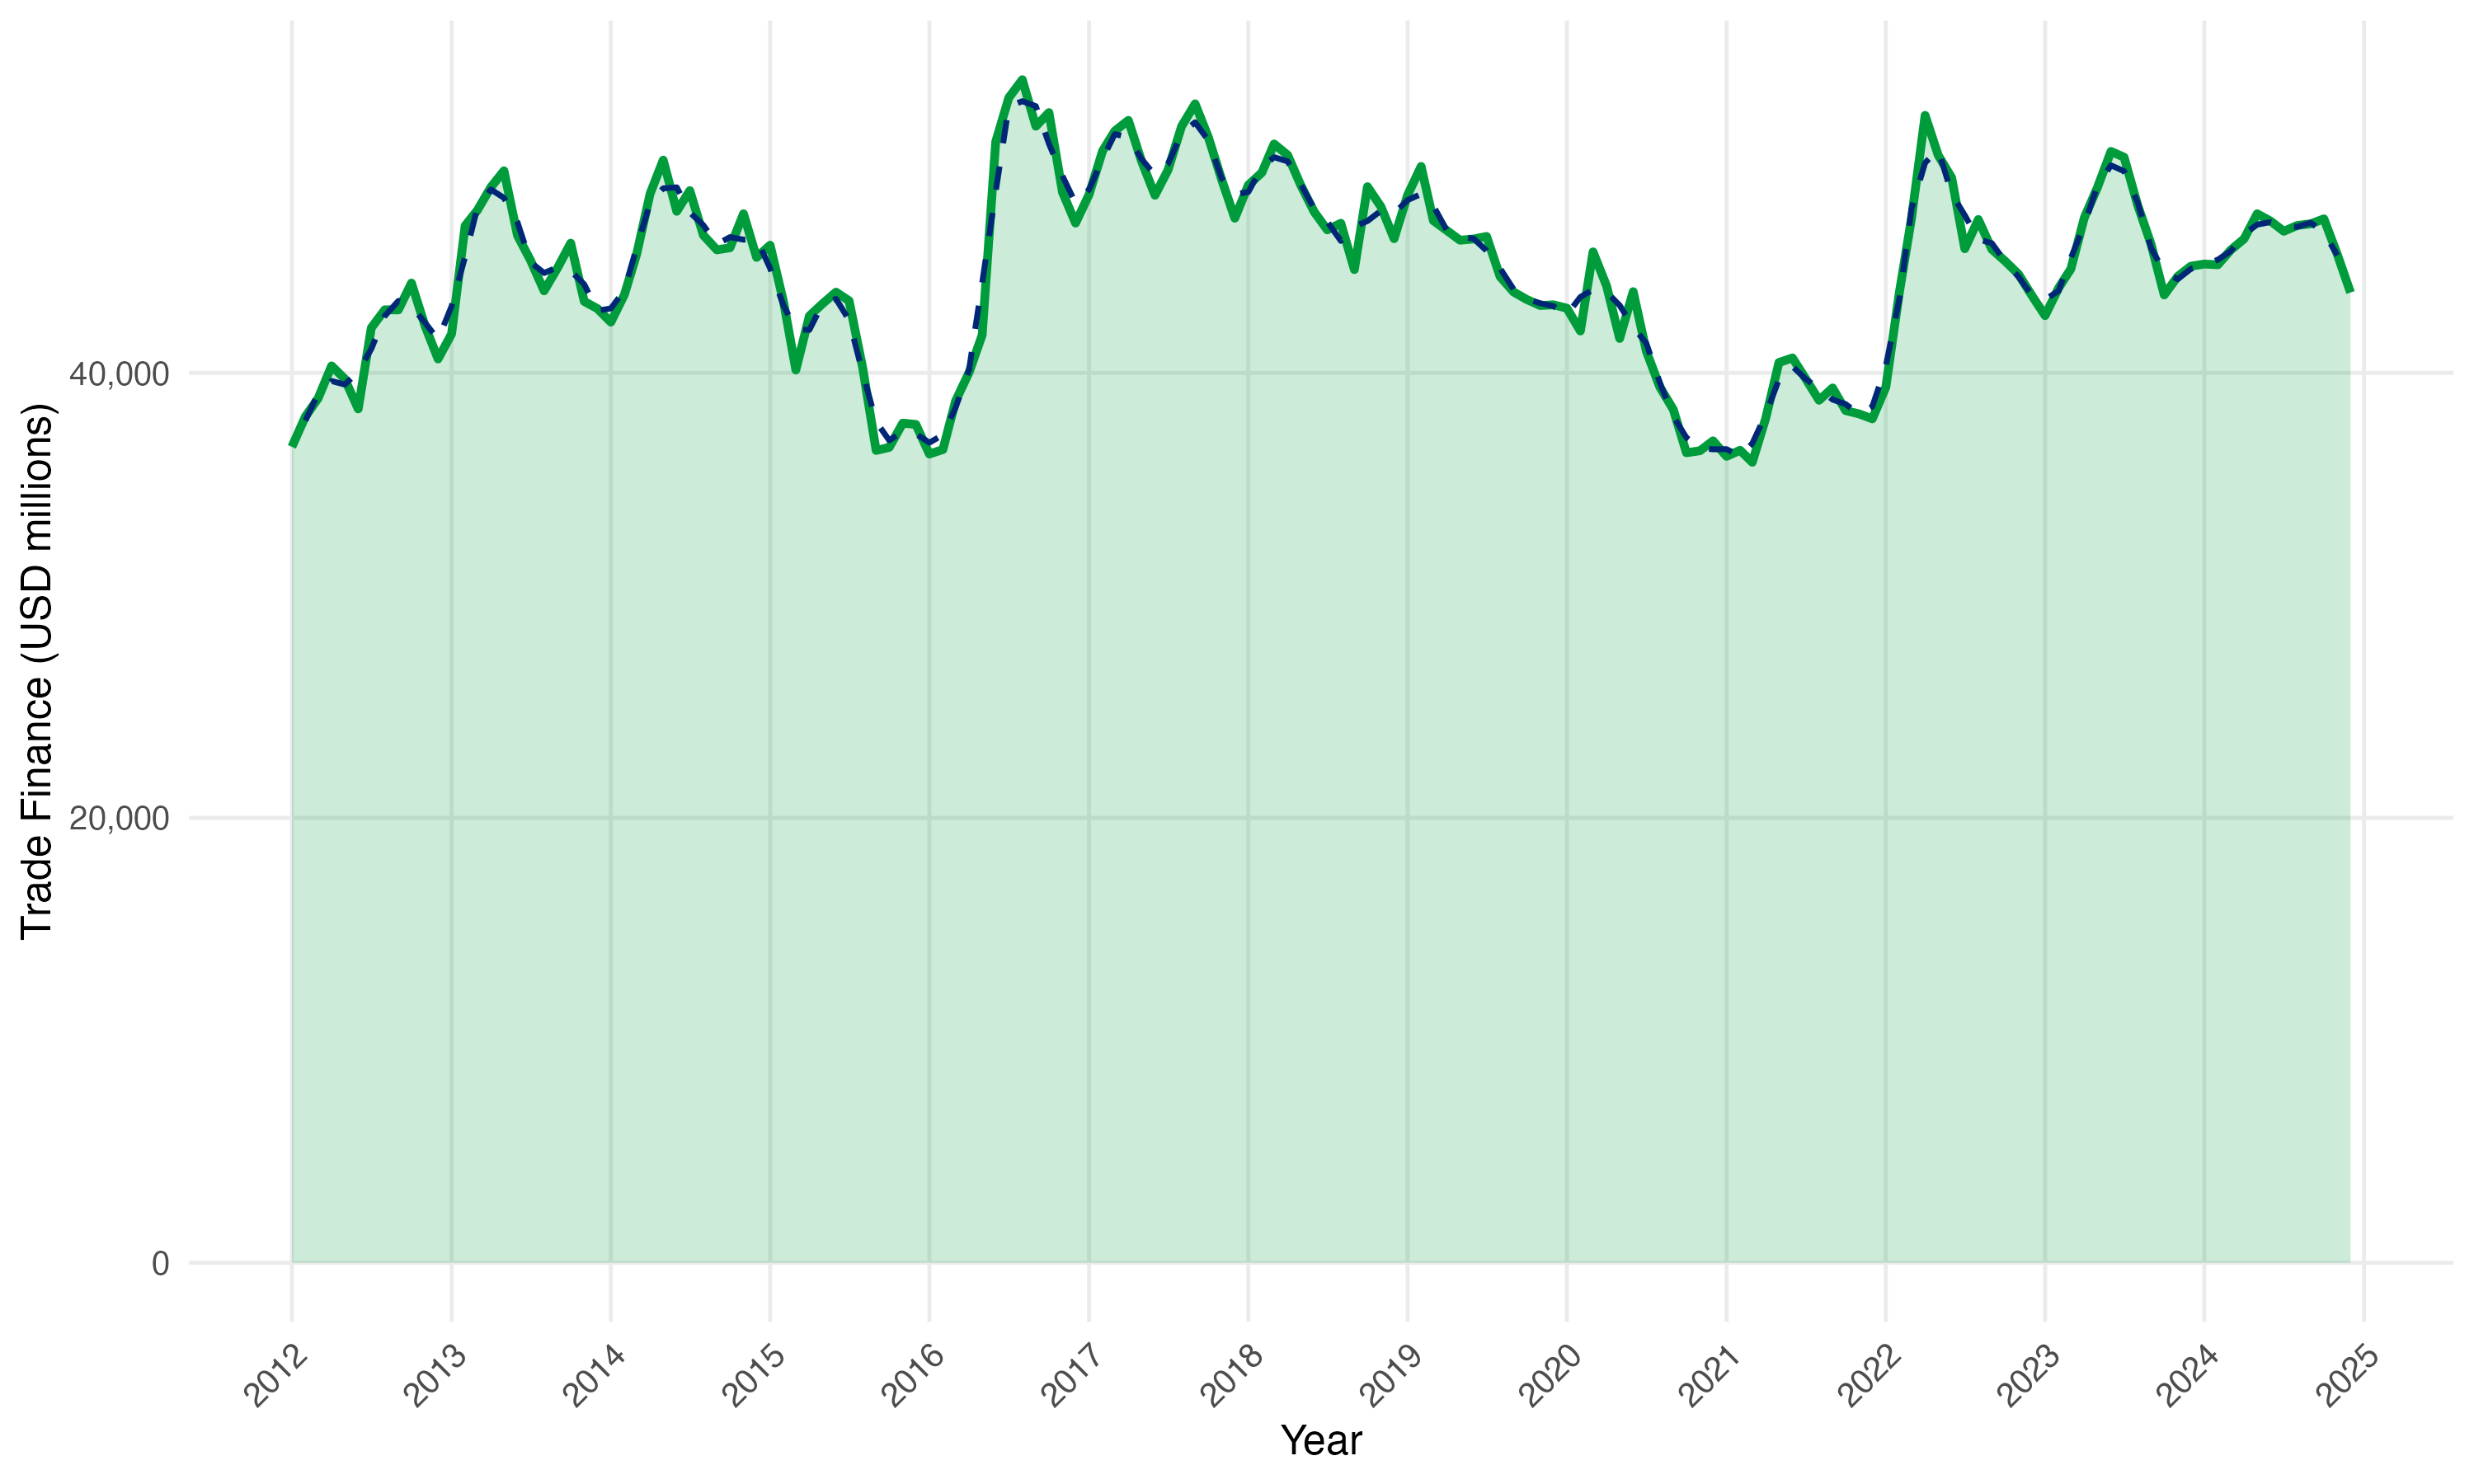
\includegraphics[width=0.7\textwidth]{plots/brazil/bra_01_tf_pct_total.png}
\end{center}
\vspace{-0.3cm}
\small
\textbf{Description:} TF credit as share of total credit. National aggregate. Monthly 2012-2024.

\vspace{0.2cm}
\textbf{Source:} BCB SCR

\vspace{0.2cm}
\textbf{Notes:} Range: 3-8\% of total credit. Includes ACC, ACE, FINIMP, NCE modalities.
\end{frame}

\begin{frame}{BRA-2: Foreign-Trade Credit by Borrower Size}
\begin{center}
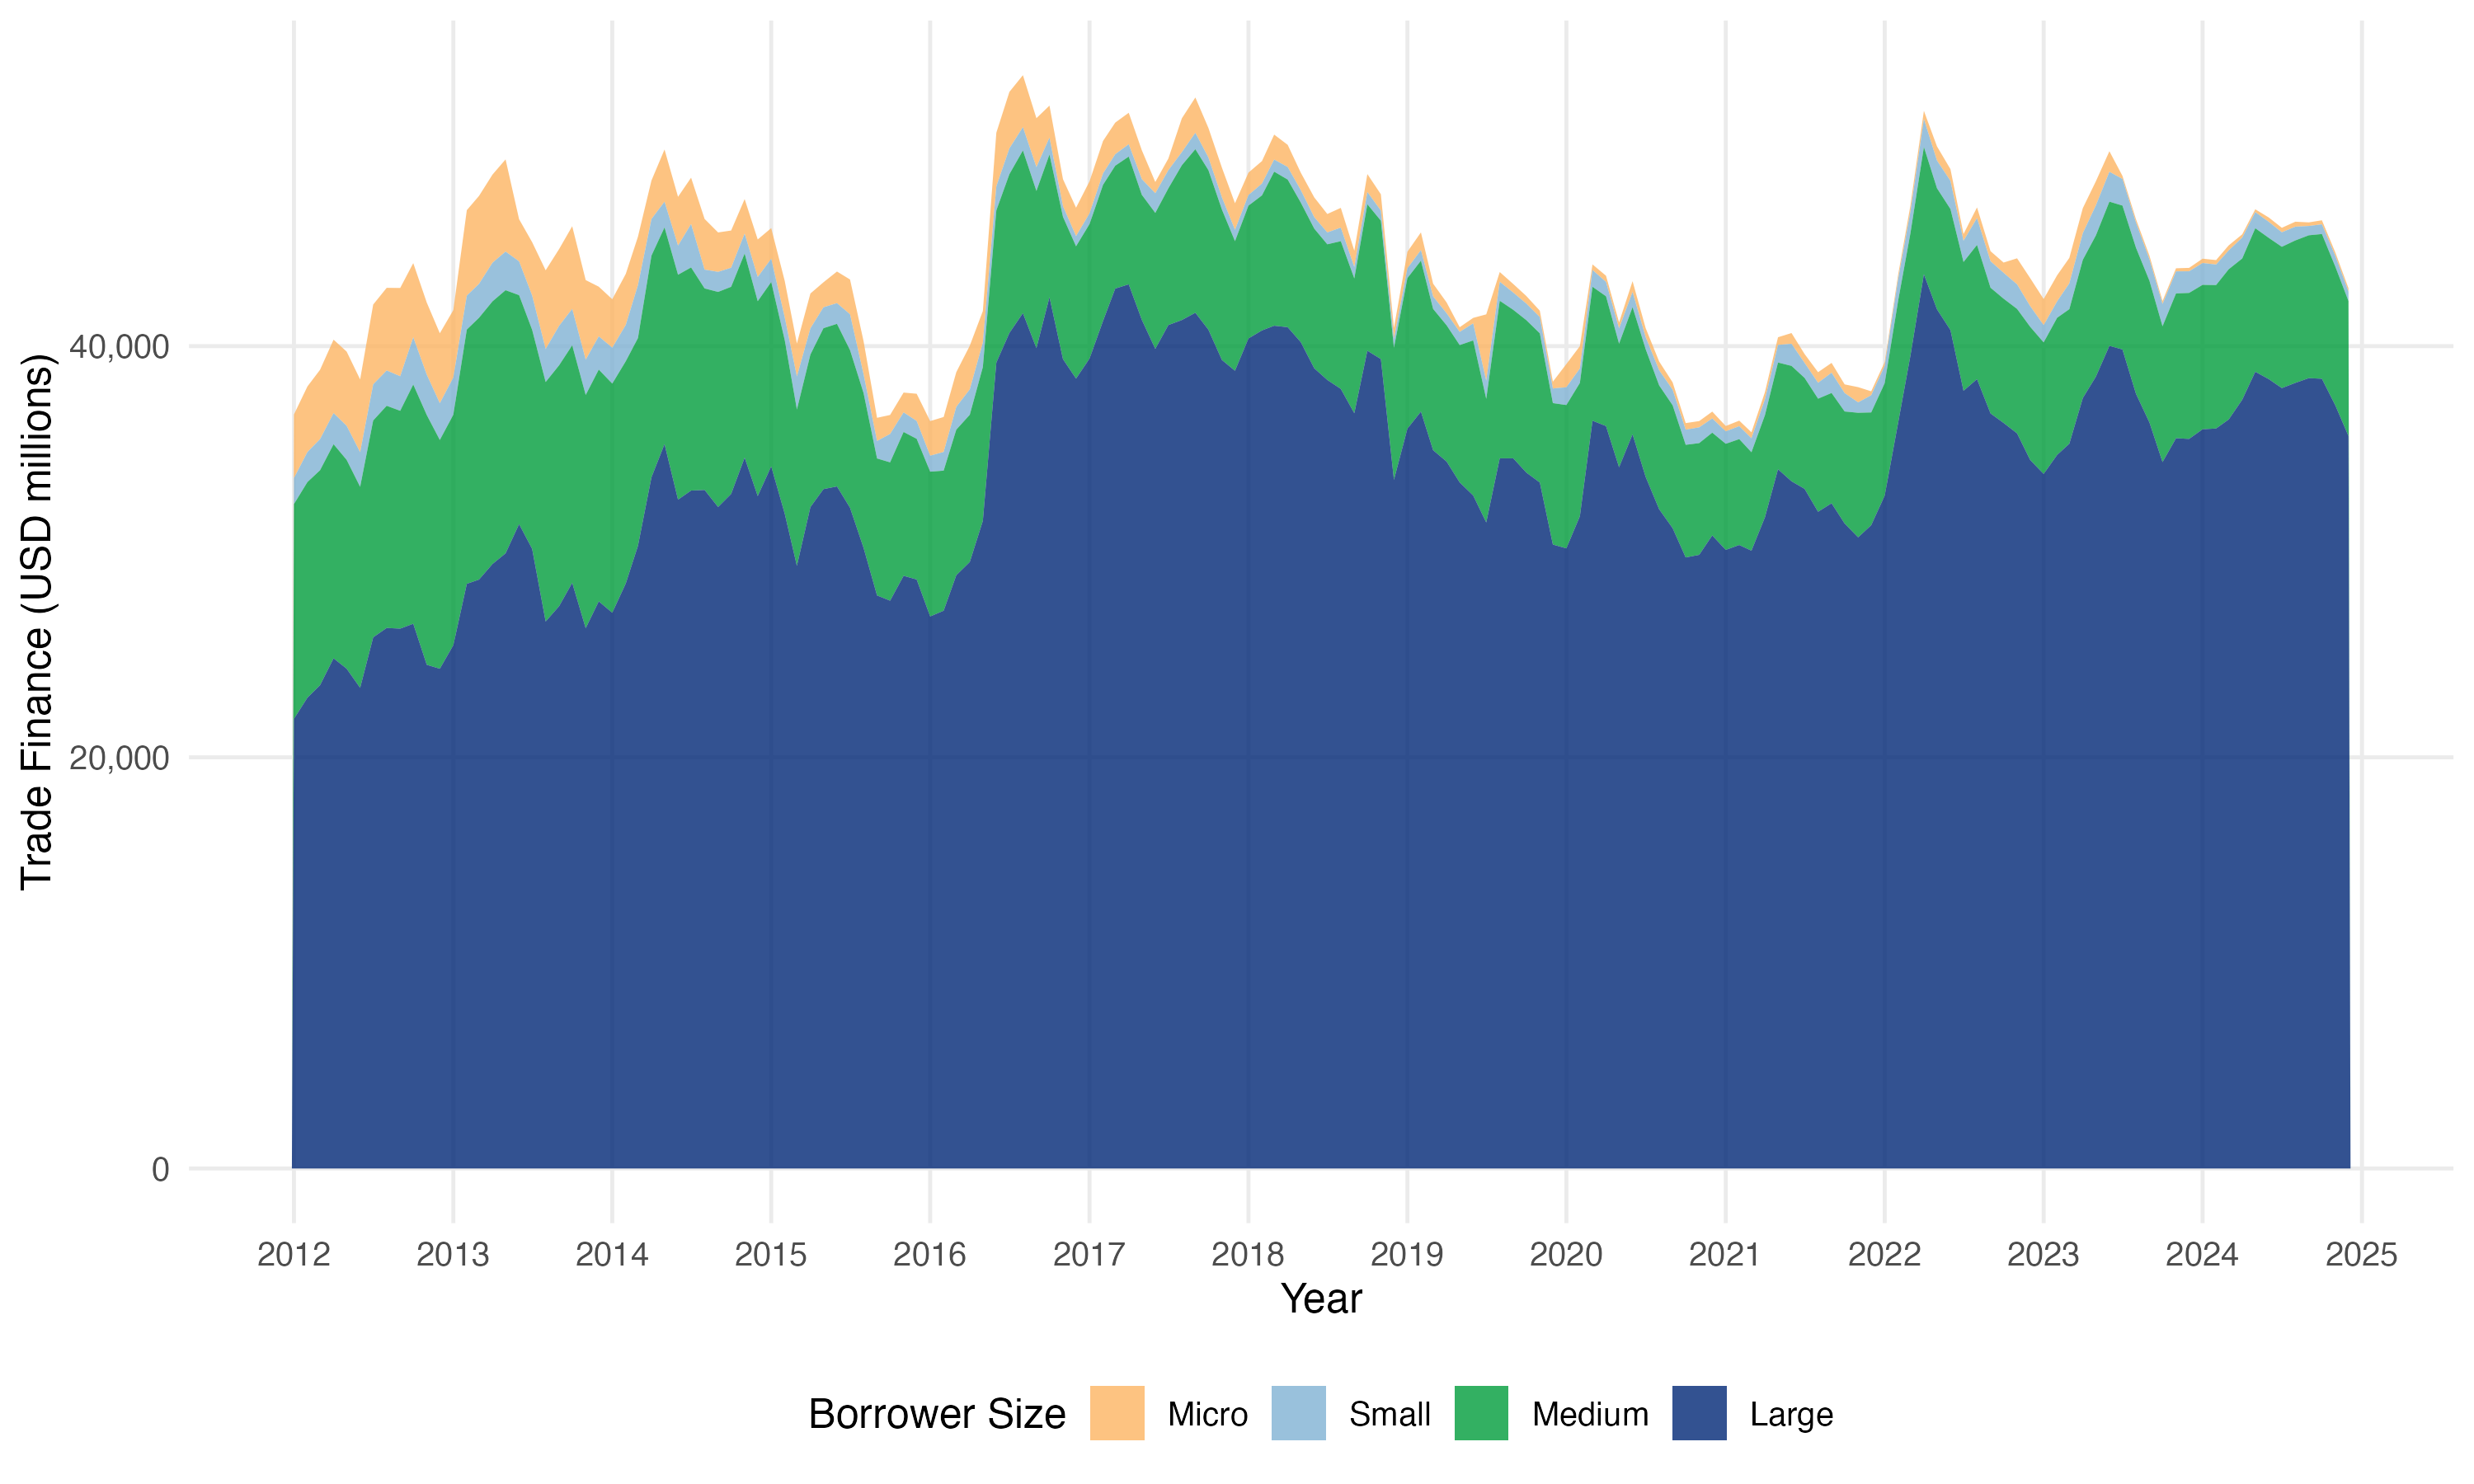
\includegraphics[width=0.7\textwidth]{plots/brazil/bra_02_tf_by_size.png}
\end{center}
\vspace{-0.3cm}
\small
\textbf{Description:} Annual grouped bars showing TF distribution across enterprise size categories. 2012-2024.

\vspace{0.2cm}
\textbf{Source:} BCB Monthly Reports

\vspace{0.2cm}
\textbf{Notes:} Size per BCB/BNDES/SEBRAE standards. Médio: 54\% by operation count. Grande: 80\% by volume.
\end{frame}

\begin{frame}{BRA-3: Foreign-Trade Credit by Region}
\begin{center}
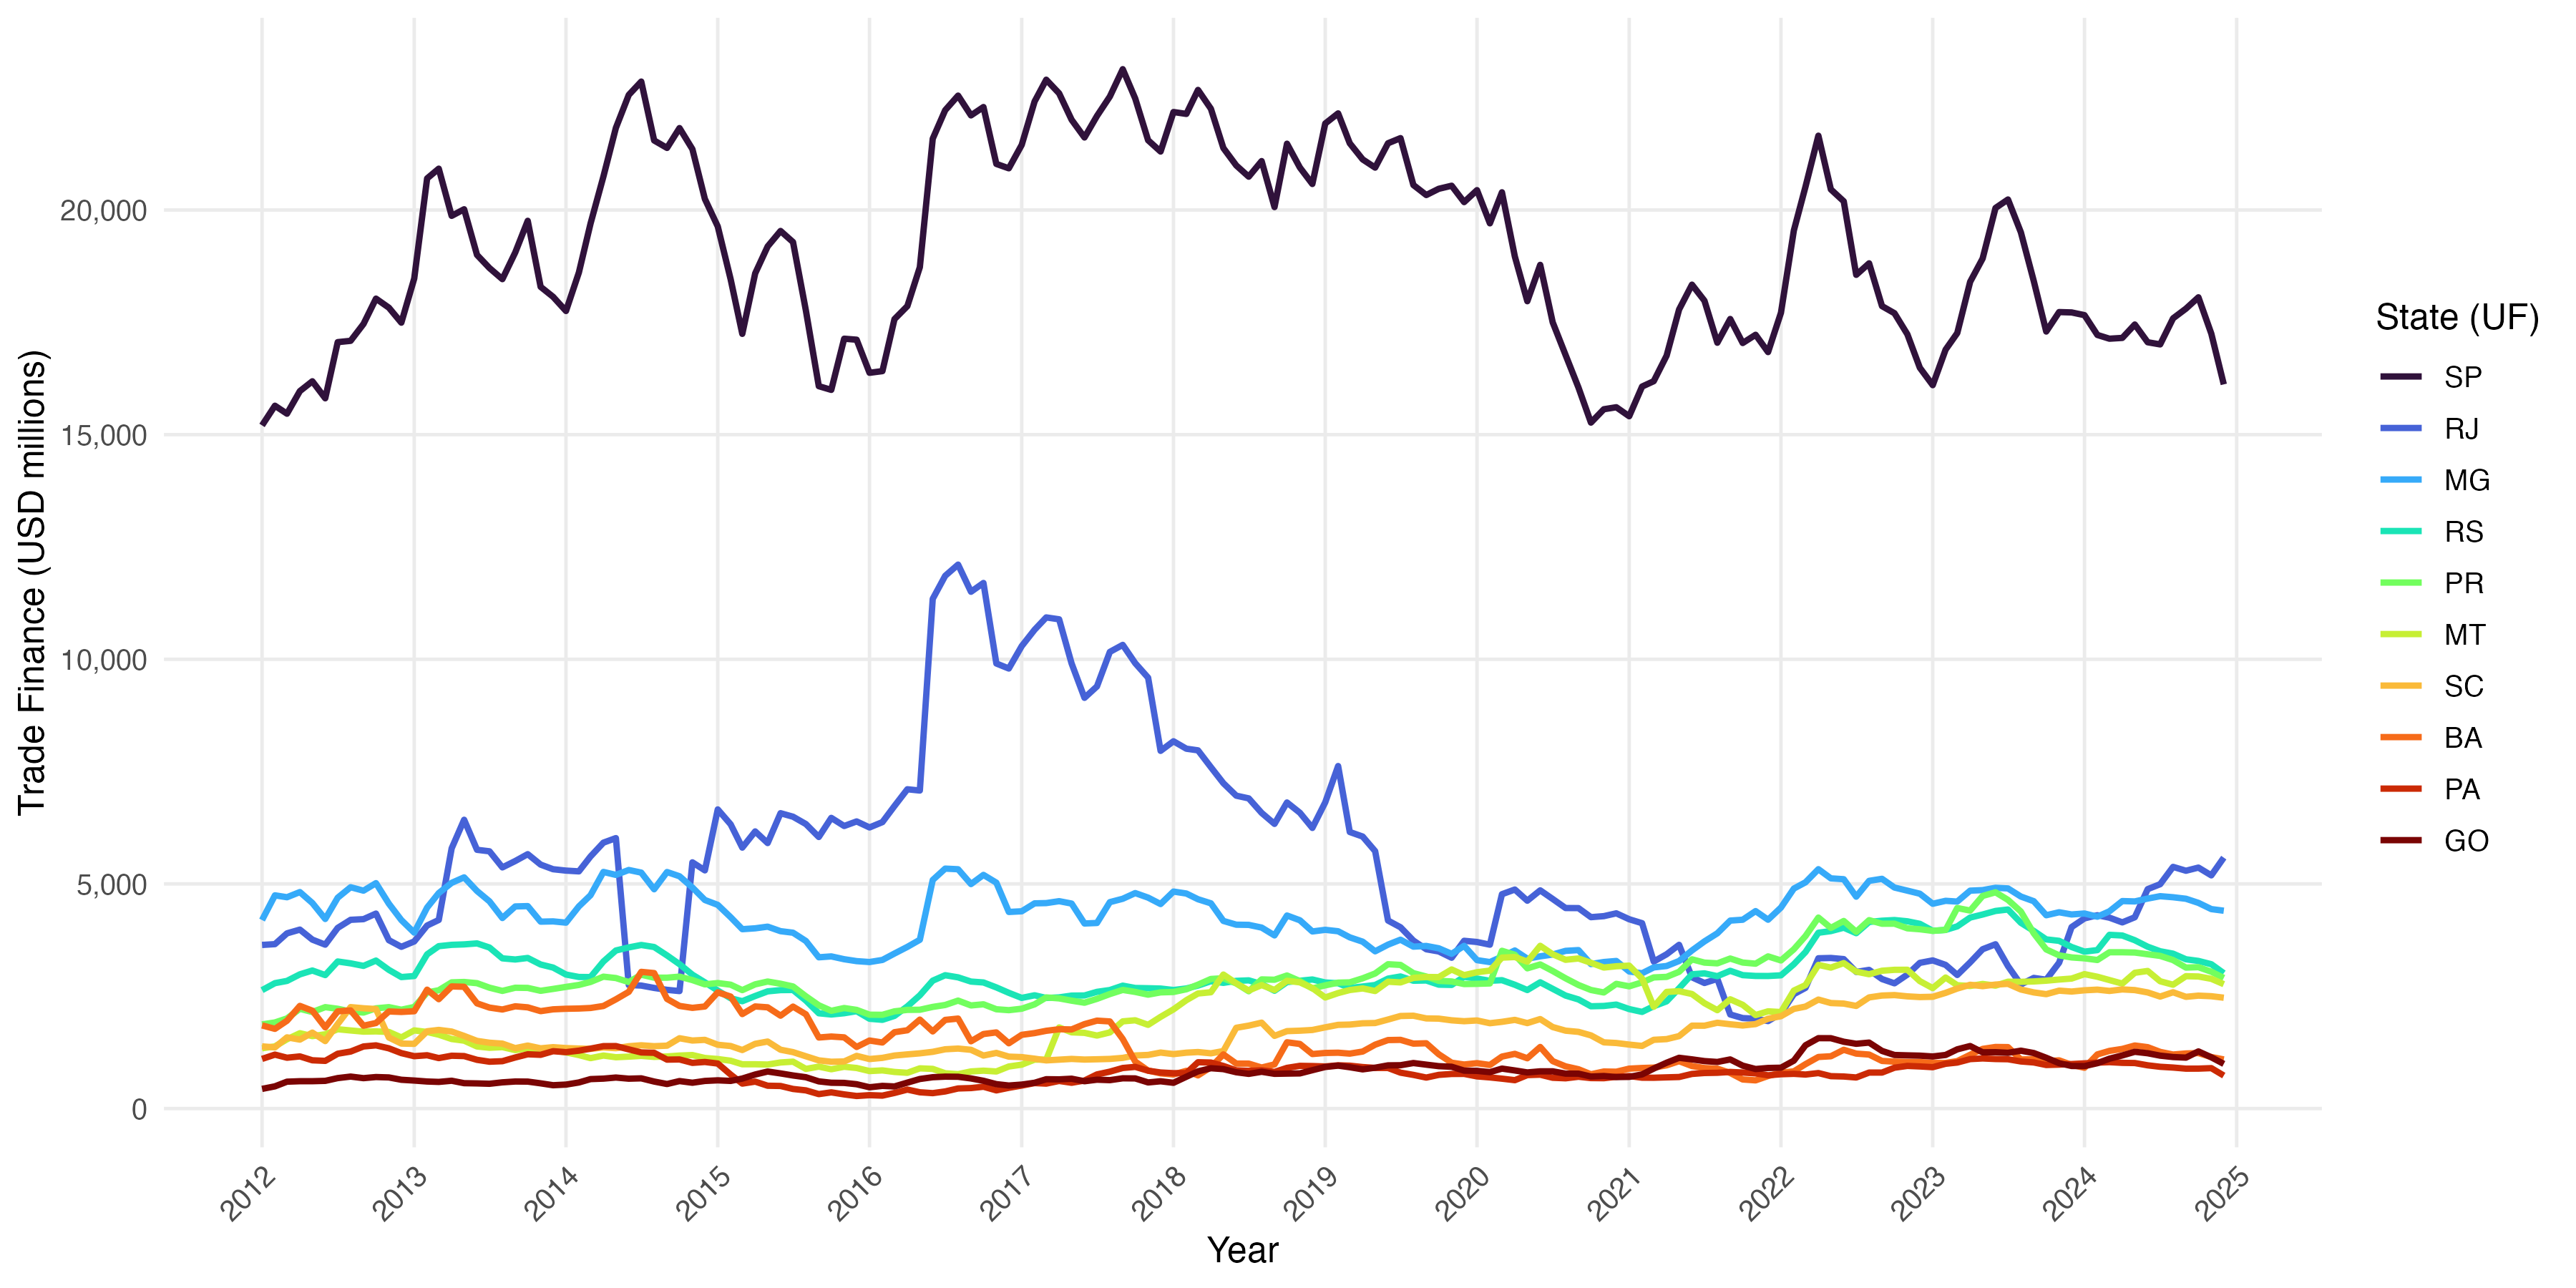
\includegraphics[width=0.7\textwidth]{plots/brazil/bra_03_tf_by_region.png}
\end{center}
\vspace{-0.3cm}
\small
\textbf{Description:} Annual grouped bars showing TF geographic distribution across Brazilian regions. 2012-2024.

\vspace{0.2cm}
\textbf{Source:} BCB Monthly Reports

\vspace{0.2cm}
\textbf{Notes:} Southeast + South: 81\% of TF. São Paulo: ~40\%. North: 2.2\%.
\end{frame}

\begin{frame}{BRA-4: Regional Concentration}
\begin{center}
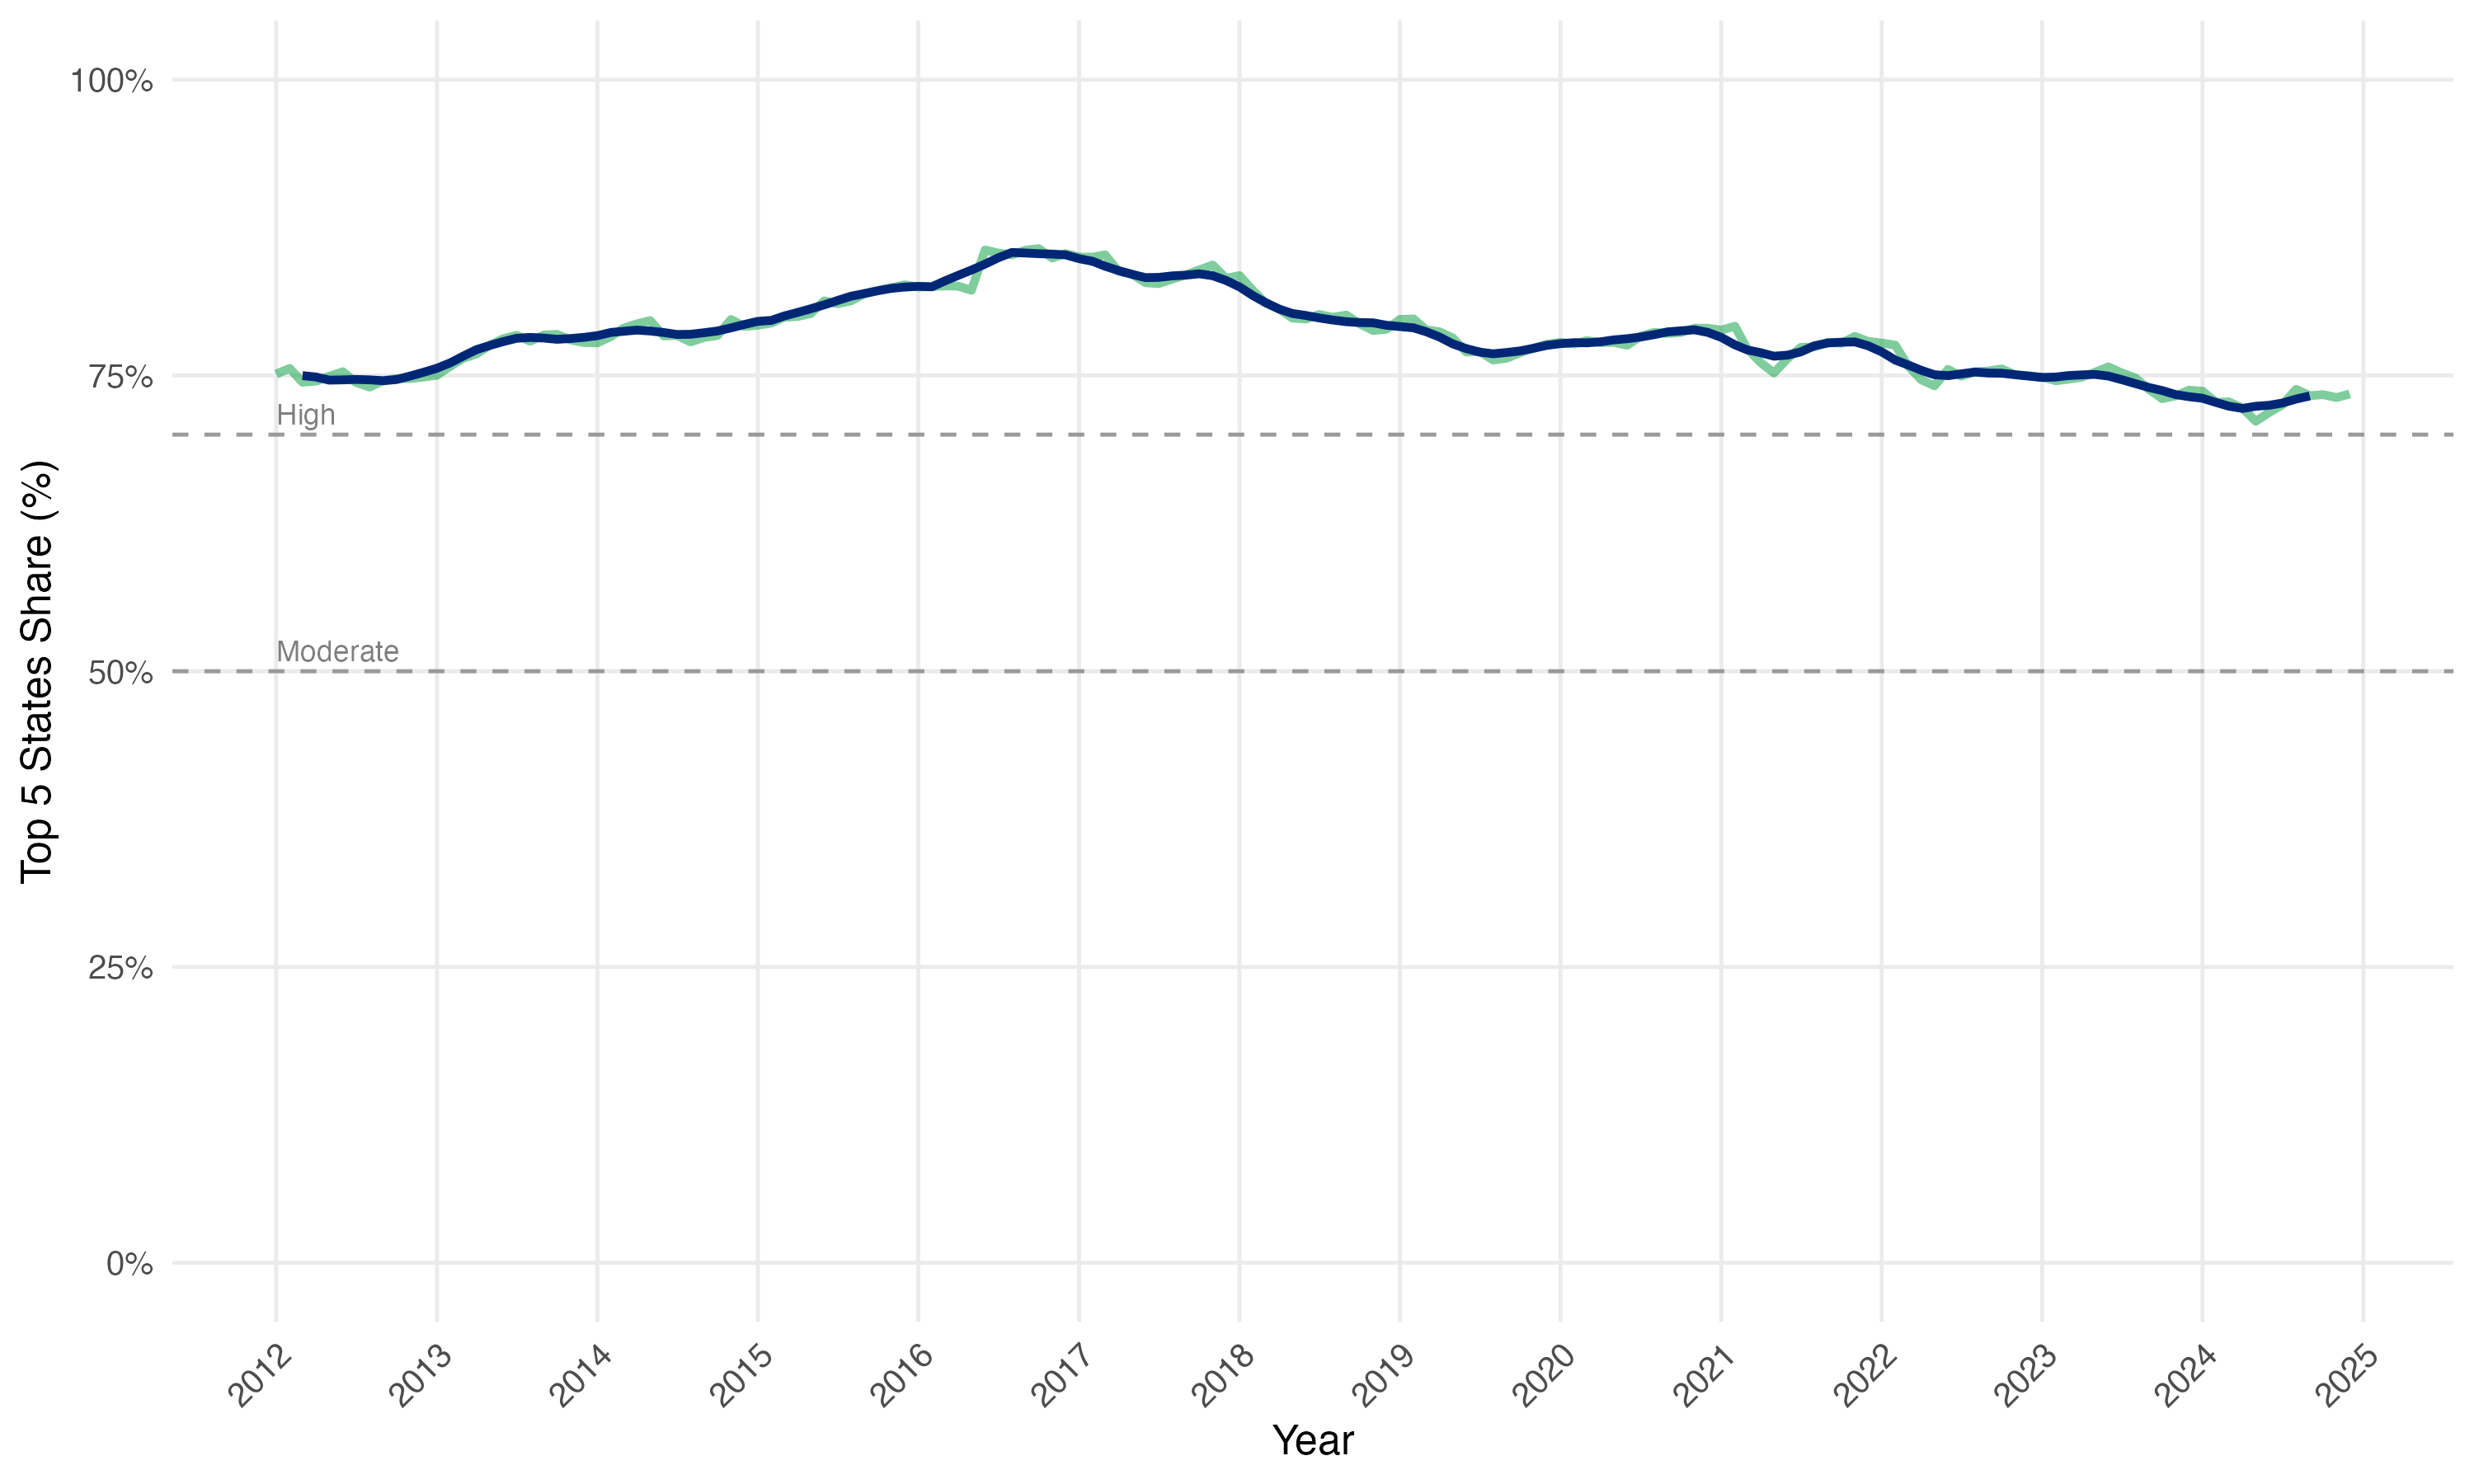
\includegraphics[width=0.7\textwidth]{plots/brazil/bra_04_regional_concentration.png}
\end{center}
\vspace{-0.3cm}
\small
\textbf{Description:} Line chart showing regional concentration metrics evolution 2012-2024.

\vspace{0.2cm}
\textbf{Source:} BCB Monthly Reports

\vspace{0.2cm}
\textbf{Notes:} Top 5 states (SP, RJ, MG, PR, SC): 72\% of national volume.
\end{frame}

\begin{frame}{BRA-5: Size Distribution Comparison: Brazil vs Peru}
\begin{center}
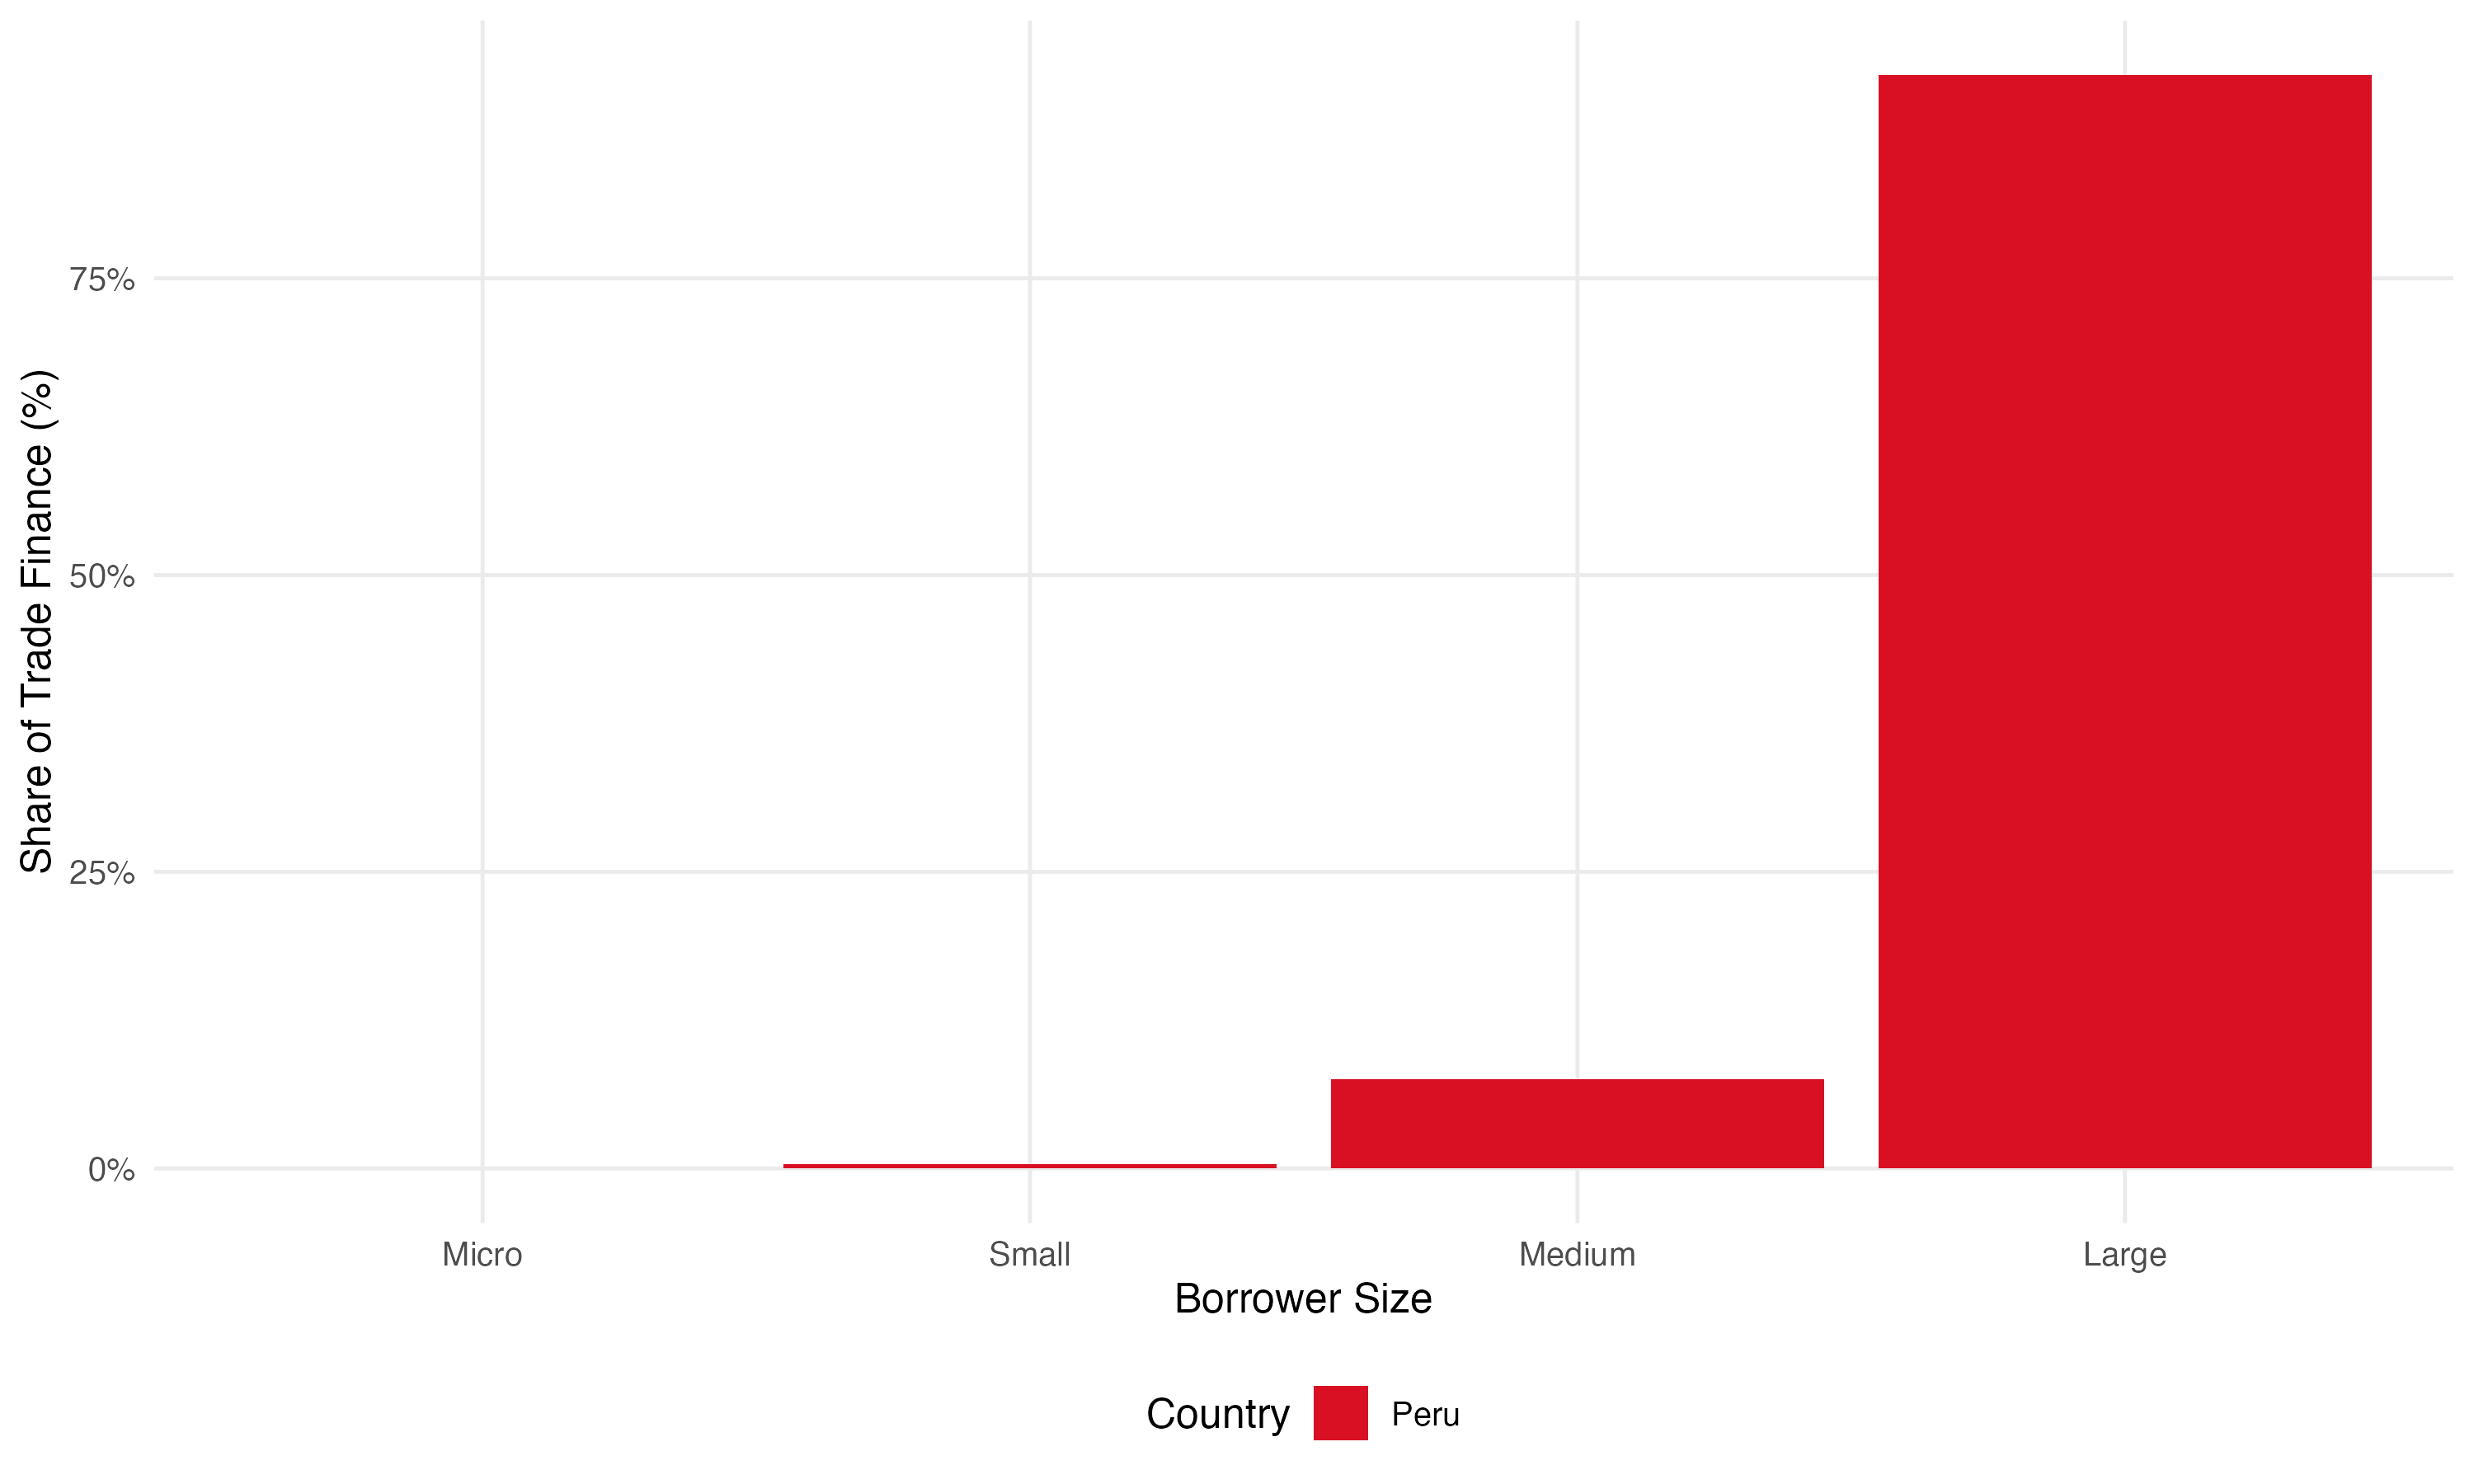
\includegraphics[width=0.7\textwidth]{plots/brazil/bra_05_size_comparison.png}
\end{center}
\vspace{-0.3cm}
\small
\textbf{Description:} Side-by-side grouped bars comparing TF borrower size distribution. 2023-2024 average.

\vspace{0.2cm}
\textbf{Source:} BCB Monthly Reports + SBS Balance de Comprobación

\vspace{0.2cm}
\textbf{Notes:} Brazil: Médio 54\%. Peru: Corporate 45\%.
\end{frame}

\begin{frame}{BRA-6: TF as \% of Annual Exports}
\begin{center}
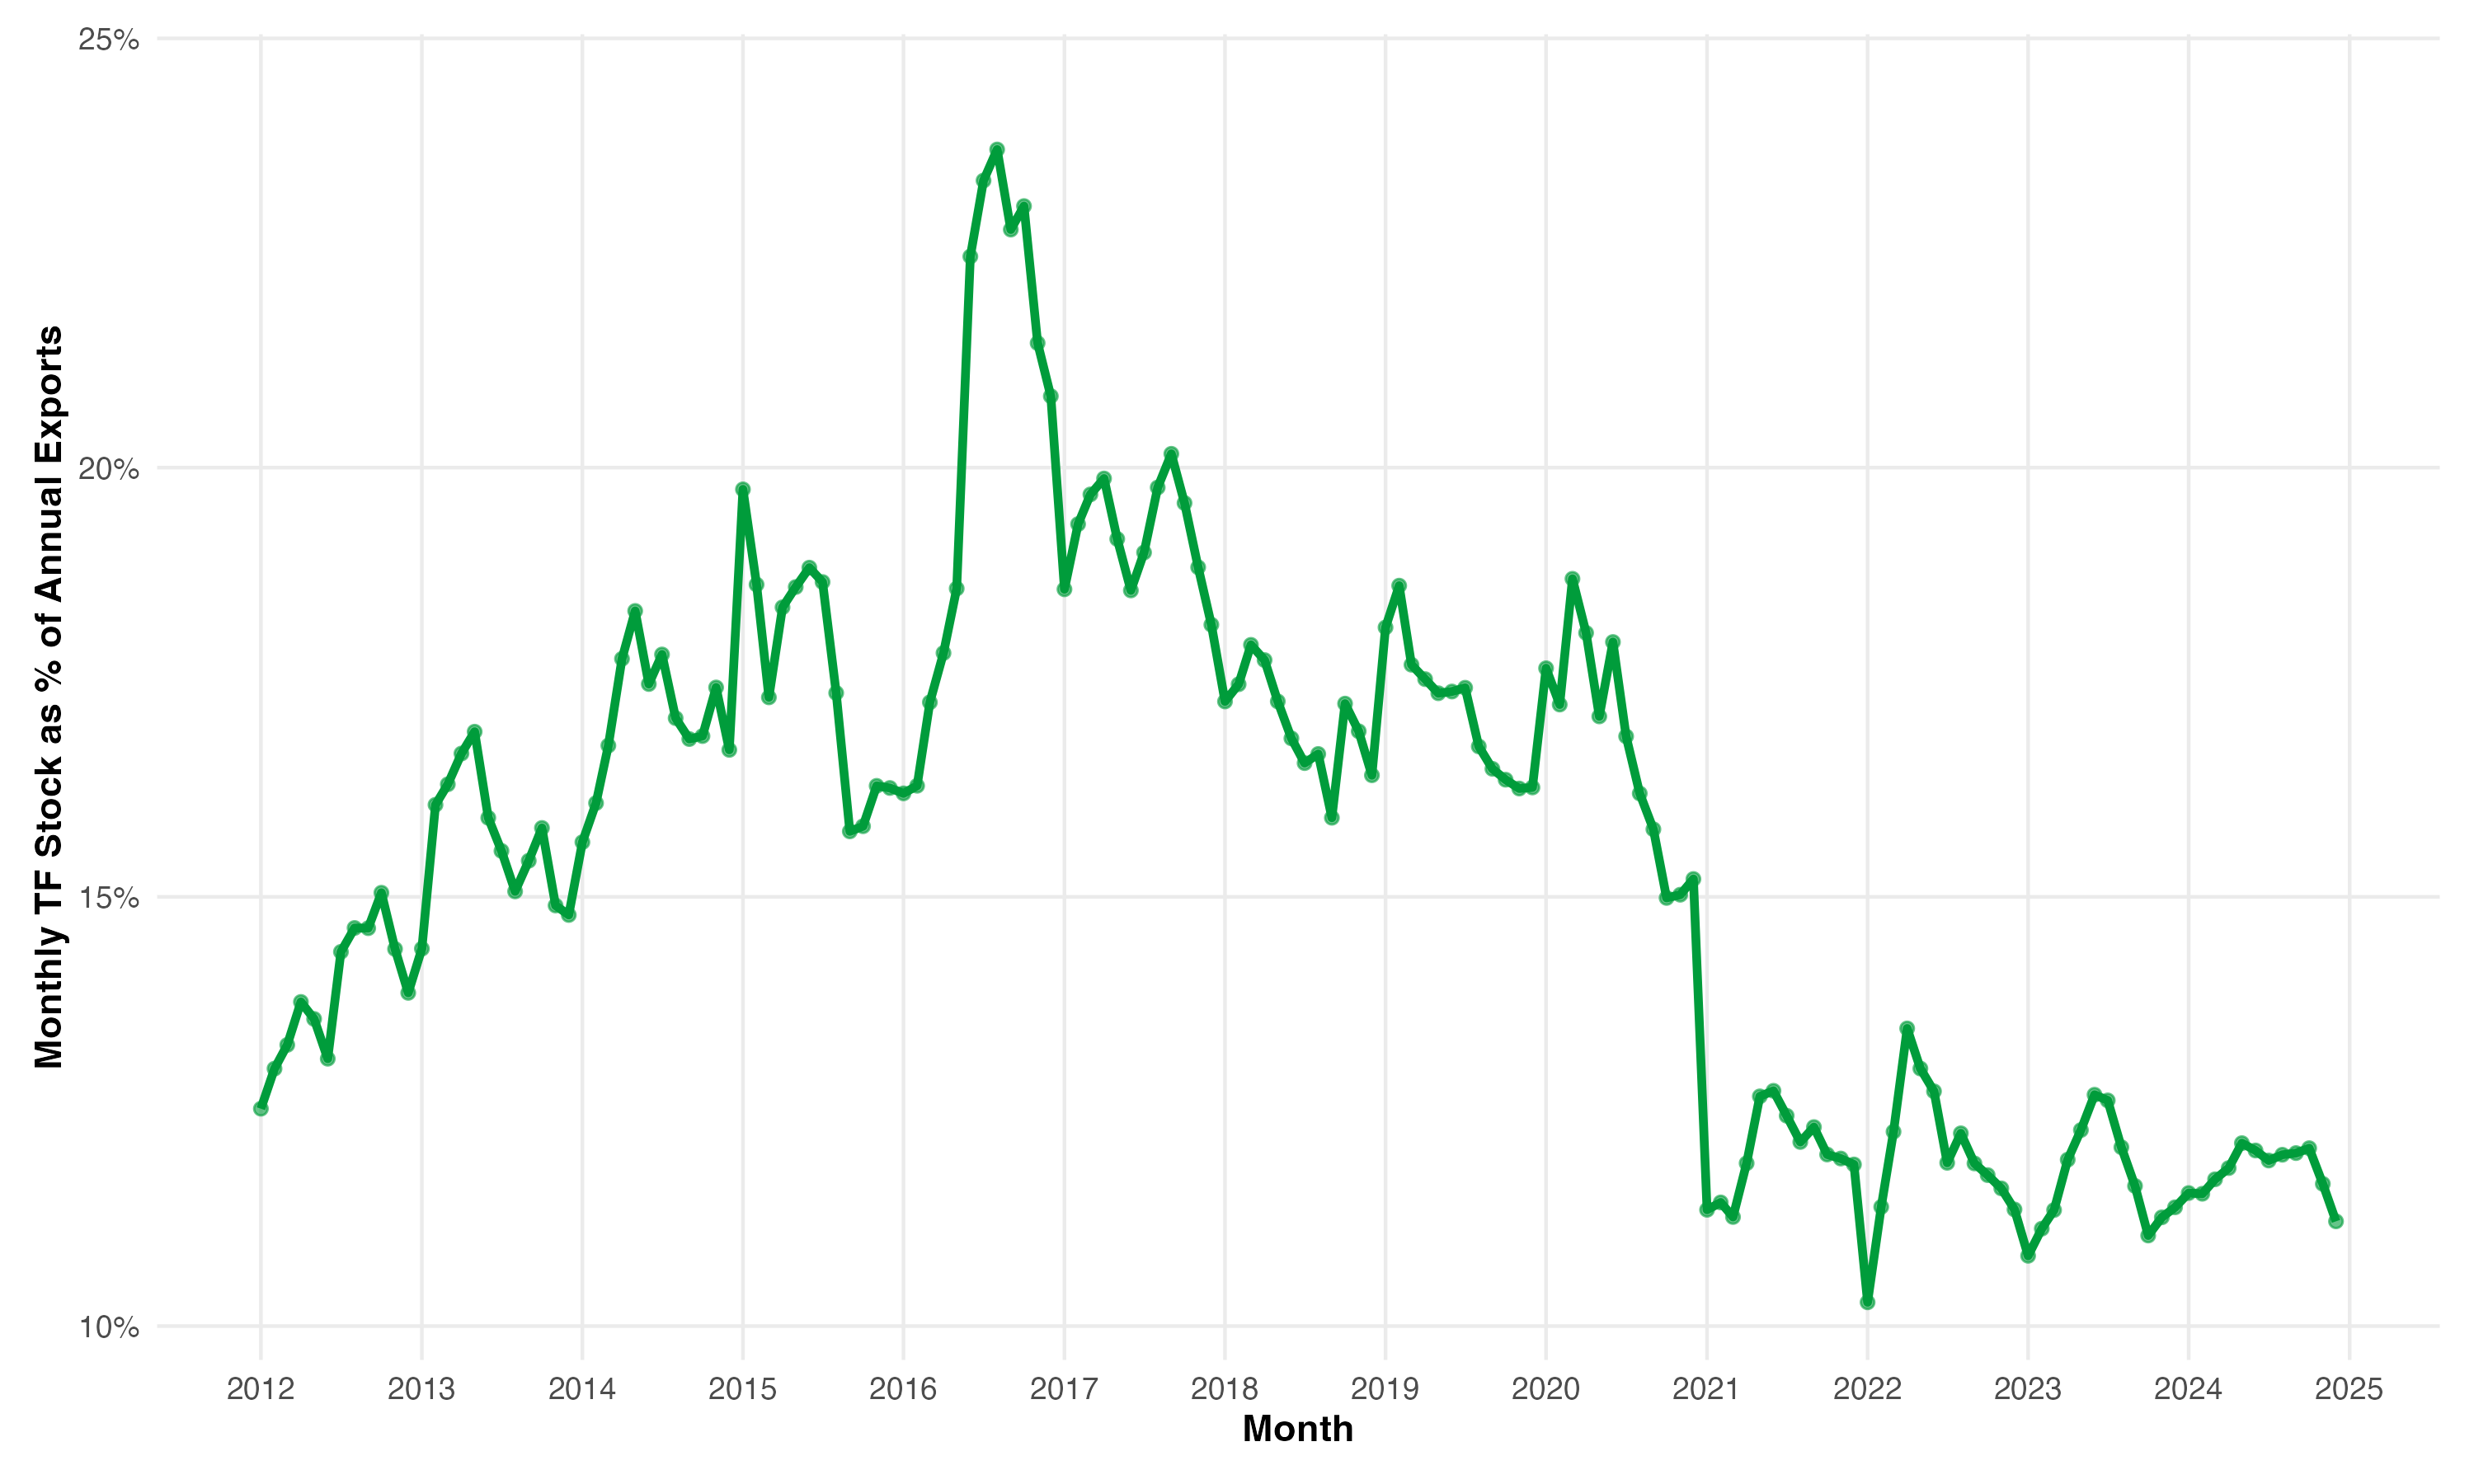
\includegraphics[width=0.7\textwidth]{plots/brazil/bra_06_tf_pct_exports.png}
\end{center}
\vspace{-0.3cm}
\small
\textbf{Description:} Monthly TF stock as percentage of annual exports. Methodology: monthly stock / annual exports × 100.

\vspace{0.2cm}
\textbf{Source:} BCB Monthly Reports + GMD

\vspace{0.2cm}
\textbf{Notes:} Range: 10.3\%-23.7\%. Decline 2020→2021 reflects commodity export boom (+31\%) with slower TF growth.
\end{frame}

\begin{frame}{BRA-7: TF as \% of Annual Total Trade}
\begin{center}
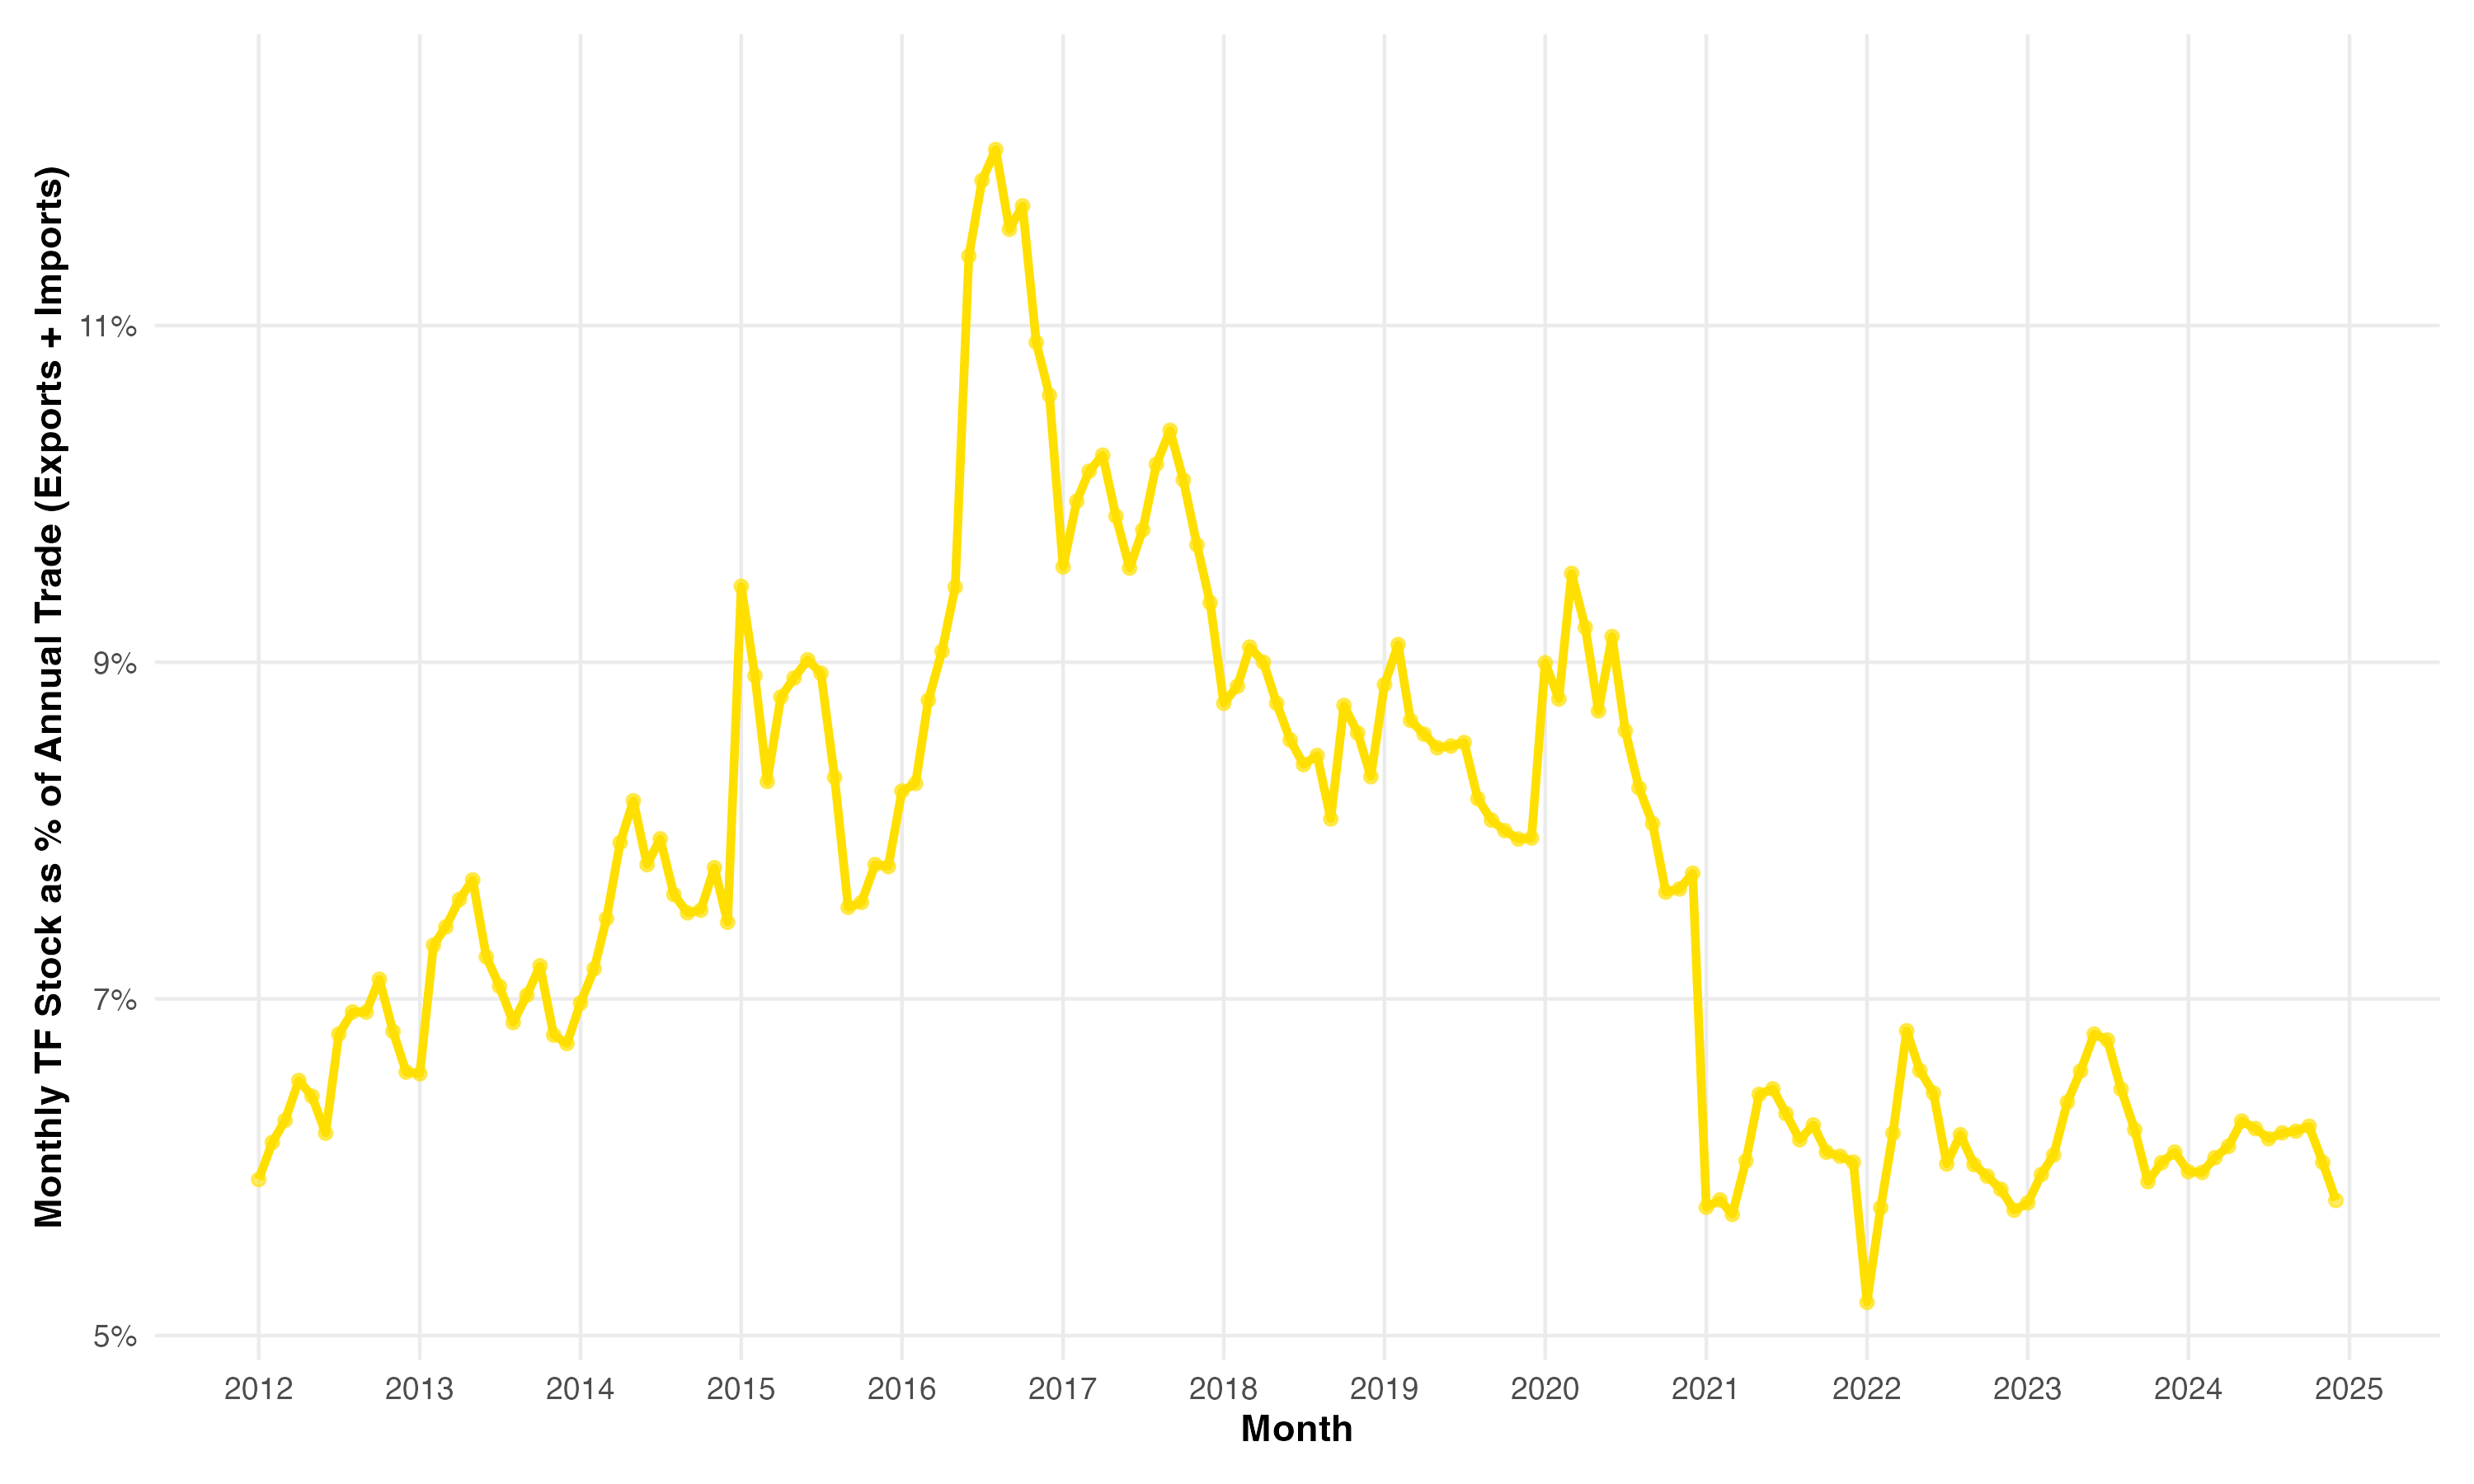
\includegraphics[width=0.7\textwidth]{plots/brazil/bra_07_tf_pct_trade.png}
\end{center}
\vspace{-0.3cm}
\small
\textbf{Description:} Monthly TF stock as percentage of annual total trade. Methodology: monthly stock / annual (X+M) × 100.

\vspace{0.2cm}
\textbf{Source:} BCB Monthly Reports + GMD

\vspace{0.2cm}
\textbf{Notes:} Range: 5.2\%-12.0\%.
\end{frame}

\begin{frame}{BRA-8: Trade Finance by Economic Sector}
\begin{center}
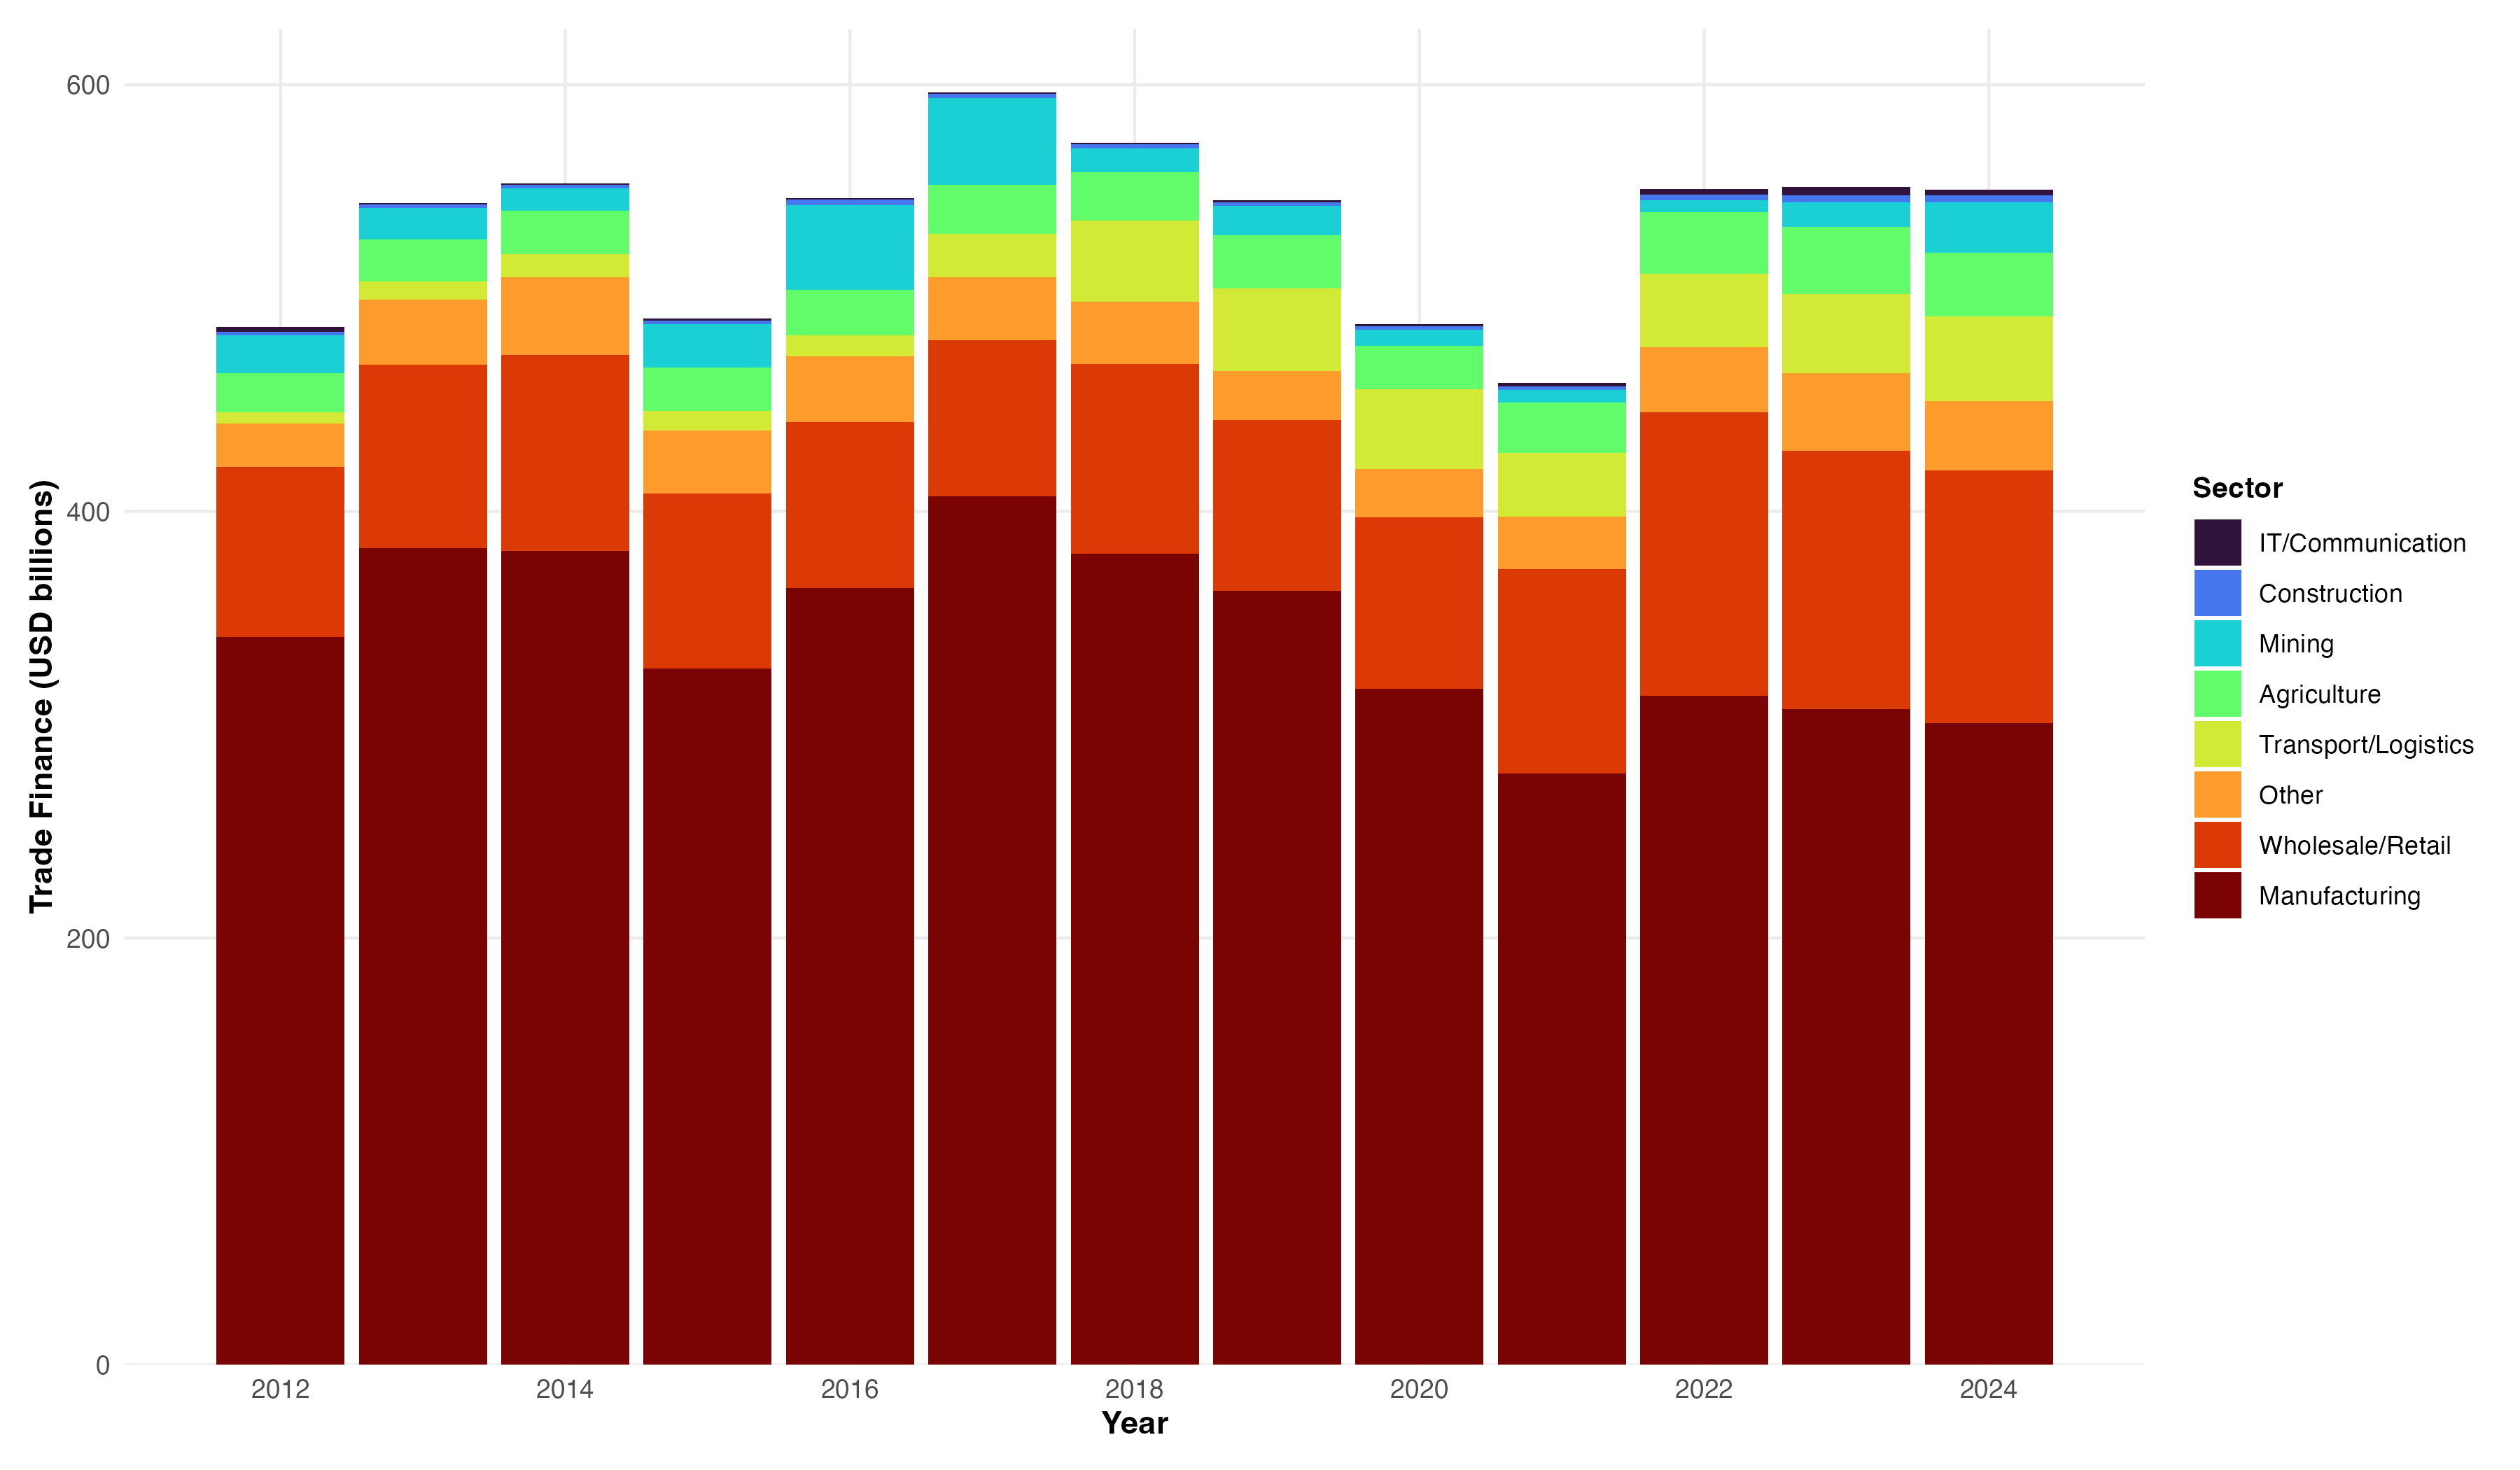
\includegraphics[width=0.7\textwidth]{plots/brazil/bra_08_tf_by_sector.png}
\end{center}
\vspace{-0.3cm}
\small
\textbf{Description:} Annual stacked bar showing TF distribution across top 10 economic sectors. 2012-2024.

\vspace{0.2cm}
\textbf{Source:} BCB Monthly Reports

\vspace{0.2cm}
\textbf{Notes:} Top 3: Manufacturing (62.9\%), Wholesale/Retail (17.0\%), Other (5.3\%).
\end{frame}

% ==============================================================================
% FINAL SLIDE
% ==============================================================================

\begin{frame}
\begin{center}
\Large
\textbf{End of Presentation}

\vspace{1cm}

\normalsize
Country Trade Finance Analysis\\
November 2025

\vspace{0.5cm}

\small
All graphs available in \texttt{plots/} directory\\
Complete captions in \texttt{captions/captions.csv}
\end{center}
\end{frame}

\end{document}
